%%____________________________________________________________________________||
\section{QCD multijet background estimation}
\label{app:qcd}

\begin{table}[h!]
  \caption{Correlation of the \bdphi and $\mht/\met$ variables, as
    determined from simulation, following the application of all other
    event selection requirements for the signal region. The
    correlation is determined per (\njet, \scalht) bins, as well as
    for inclusive \njet and \nb (``all'') categories.}
  \label{tab:bdphi_mhtmet_correlation}
  \centering
  \footnotesize
  \begin{tabular}{l|rrrrrr}
    \njet / \scalht & all & $200$ & $400$ & $600$ & $900$ & $1200$ \\
    \hline
    all  & $0.44$ & $0.33$ & $ 0.27$ & $0.48$ & $ 0.24$ & $ 0.16$ \\
    eq1j & $0.00$ & $0.00$ & $ 0.00$ & $0.00$ & $ 0.00$ & $ 0.00$ \\
    eq2j & $0.29$ & $0.27$ & $-0.09$ & $0.00$ & $-0.15$ & $ 0.44$ \\
    eq3j & $0.10$ & $0.19$ & $ 0.27$ & $0.46$ & $ 0.22$ & $ 0.12$ \\
    eq4j & $0.33$ & $0.00$ & $ 0.30$ & $0.55$ & $ 0.23$ & $ 0.22$ \\
    eq5j & $0.11$ & $0.00$ & $ 0.09$ & $0.44$ & $ 0.43$ & $ 0.12$ \\
    ge6j & $0.29$ & $0.00$ & $ 0.08$ & $0.54$ & $ 0.18$ & $-0.01$ \\
    ge2a & $0.21$ & $0.16$ & $ 0.31$ & $1.00$ & $ 0.00$ & $ 0.00$ \\
  \end{tabular}
\end{table}

\clearpage
\begin{figure}[!h]
  \centering
  \subfigure[Sideband \textbf{B} \scalht distribution]{
    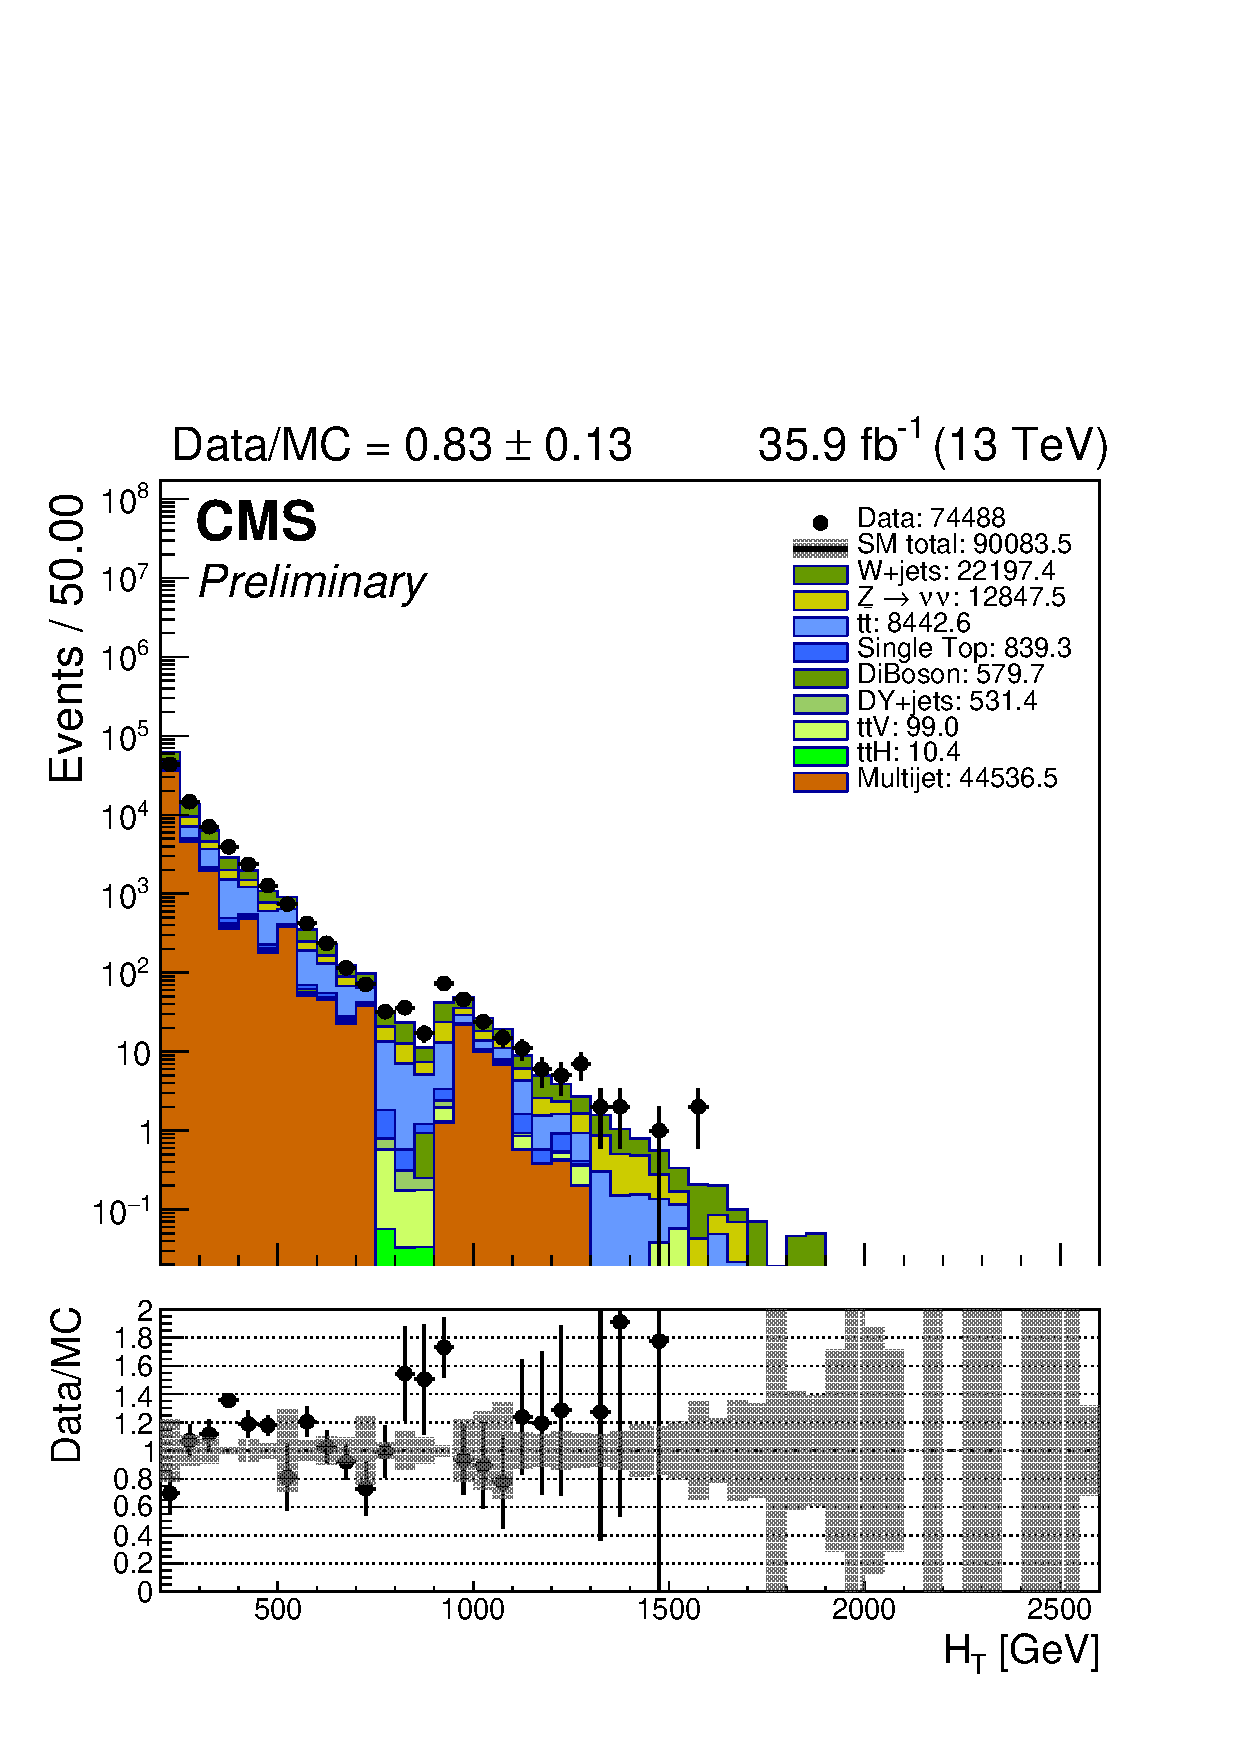
\includegraphics[width=0.5\textwidth]{figures/qcd/distributions/mhtmetsb_ht40}
  }
  \subfigure[Sideband \textbf{B} \njet distribution]{
    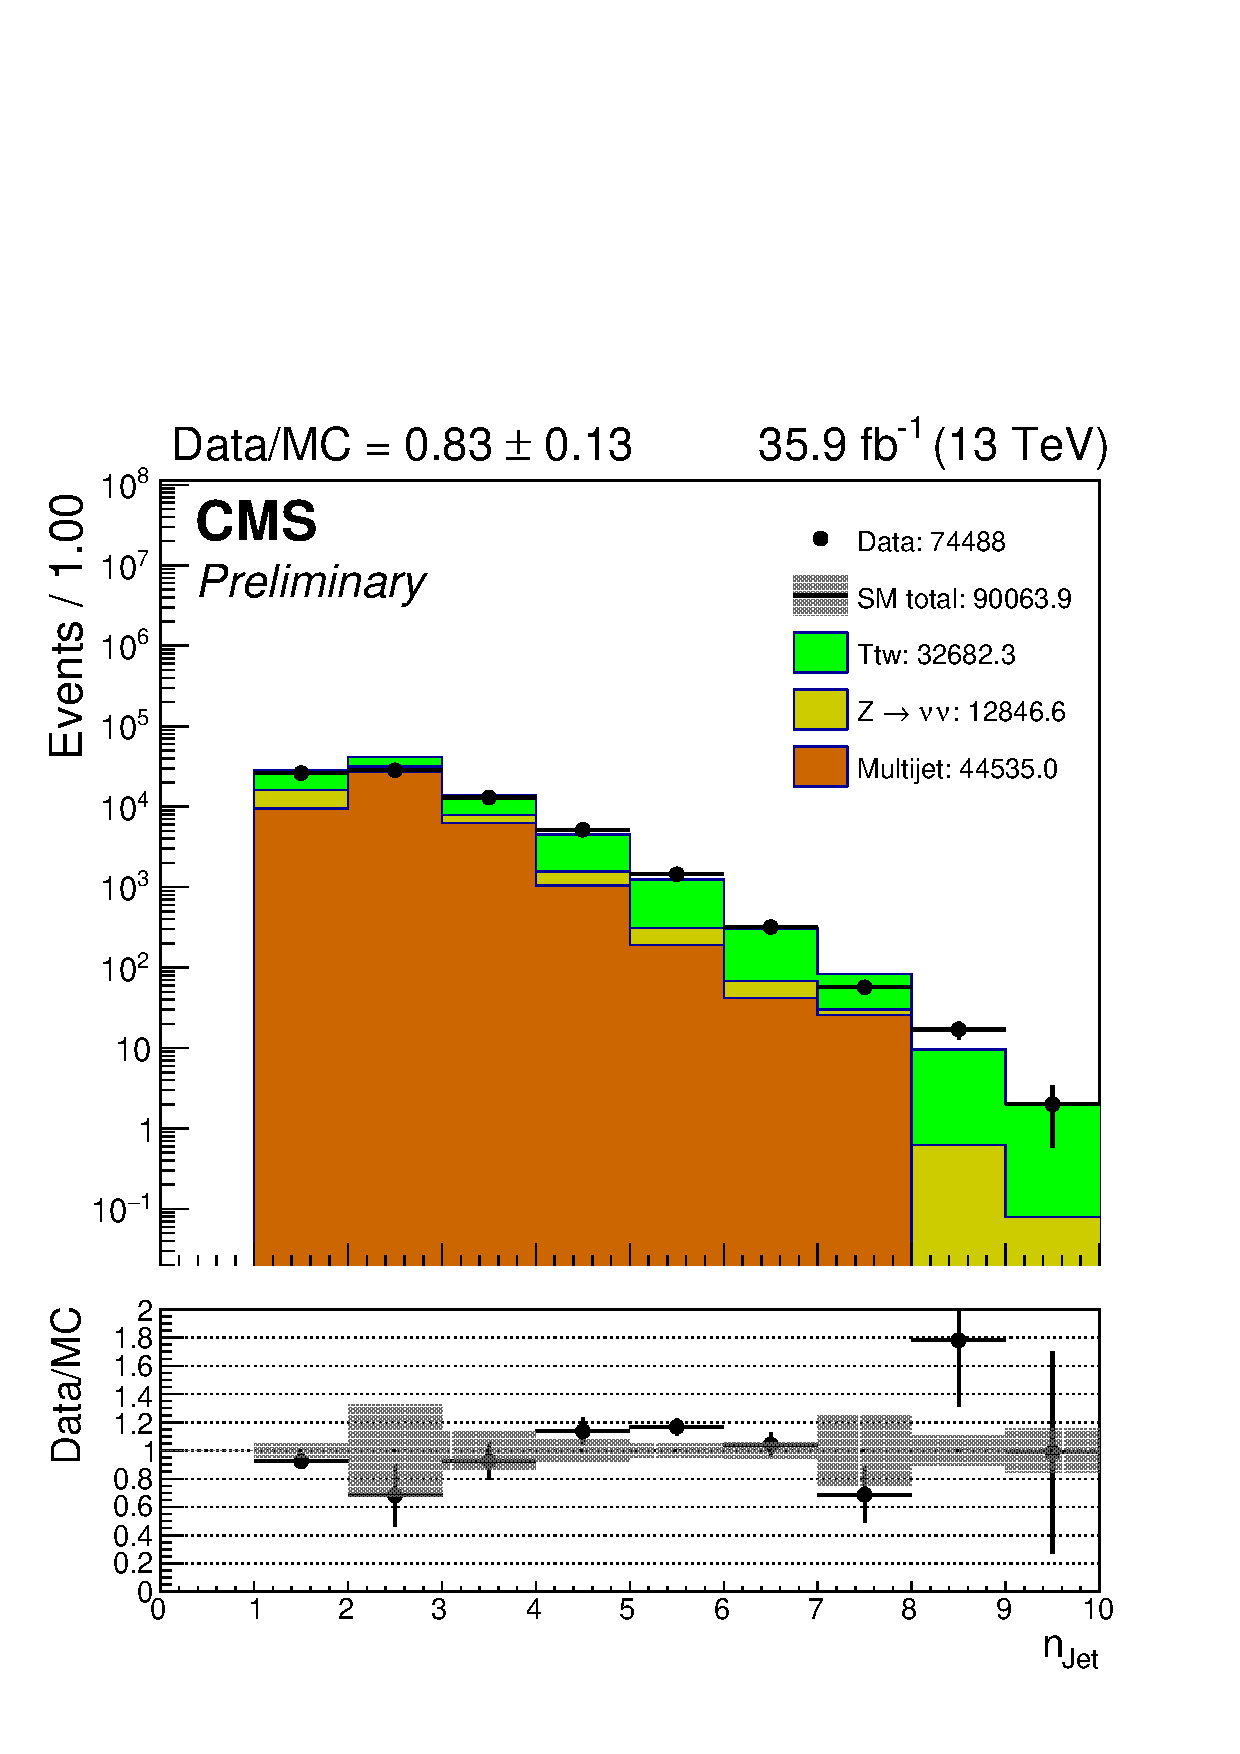
\includegraphics[width=0.5\textwidth]{figures/qcd/distributions/mhtmetsb_njet40}
  } \\
  \subfigure[Sideband \textbf{C} \scalht distribution]{
    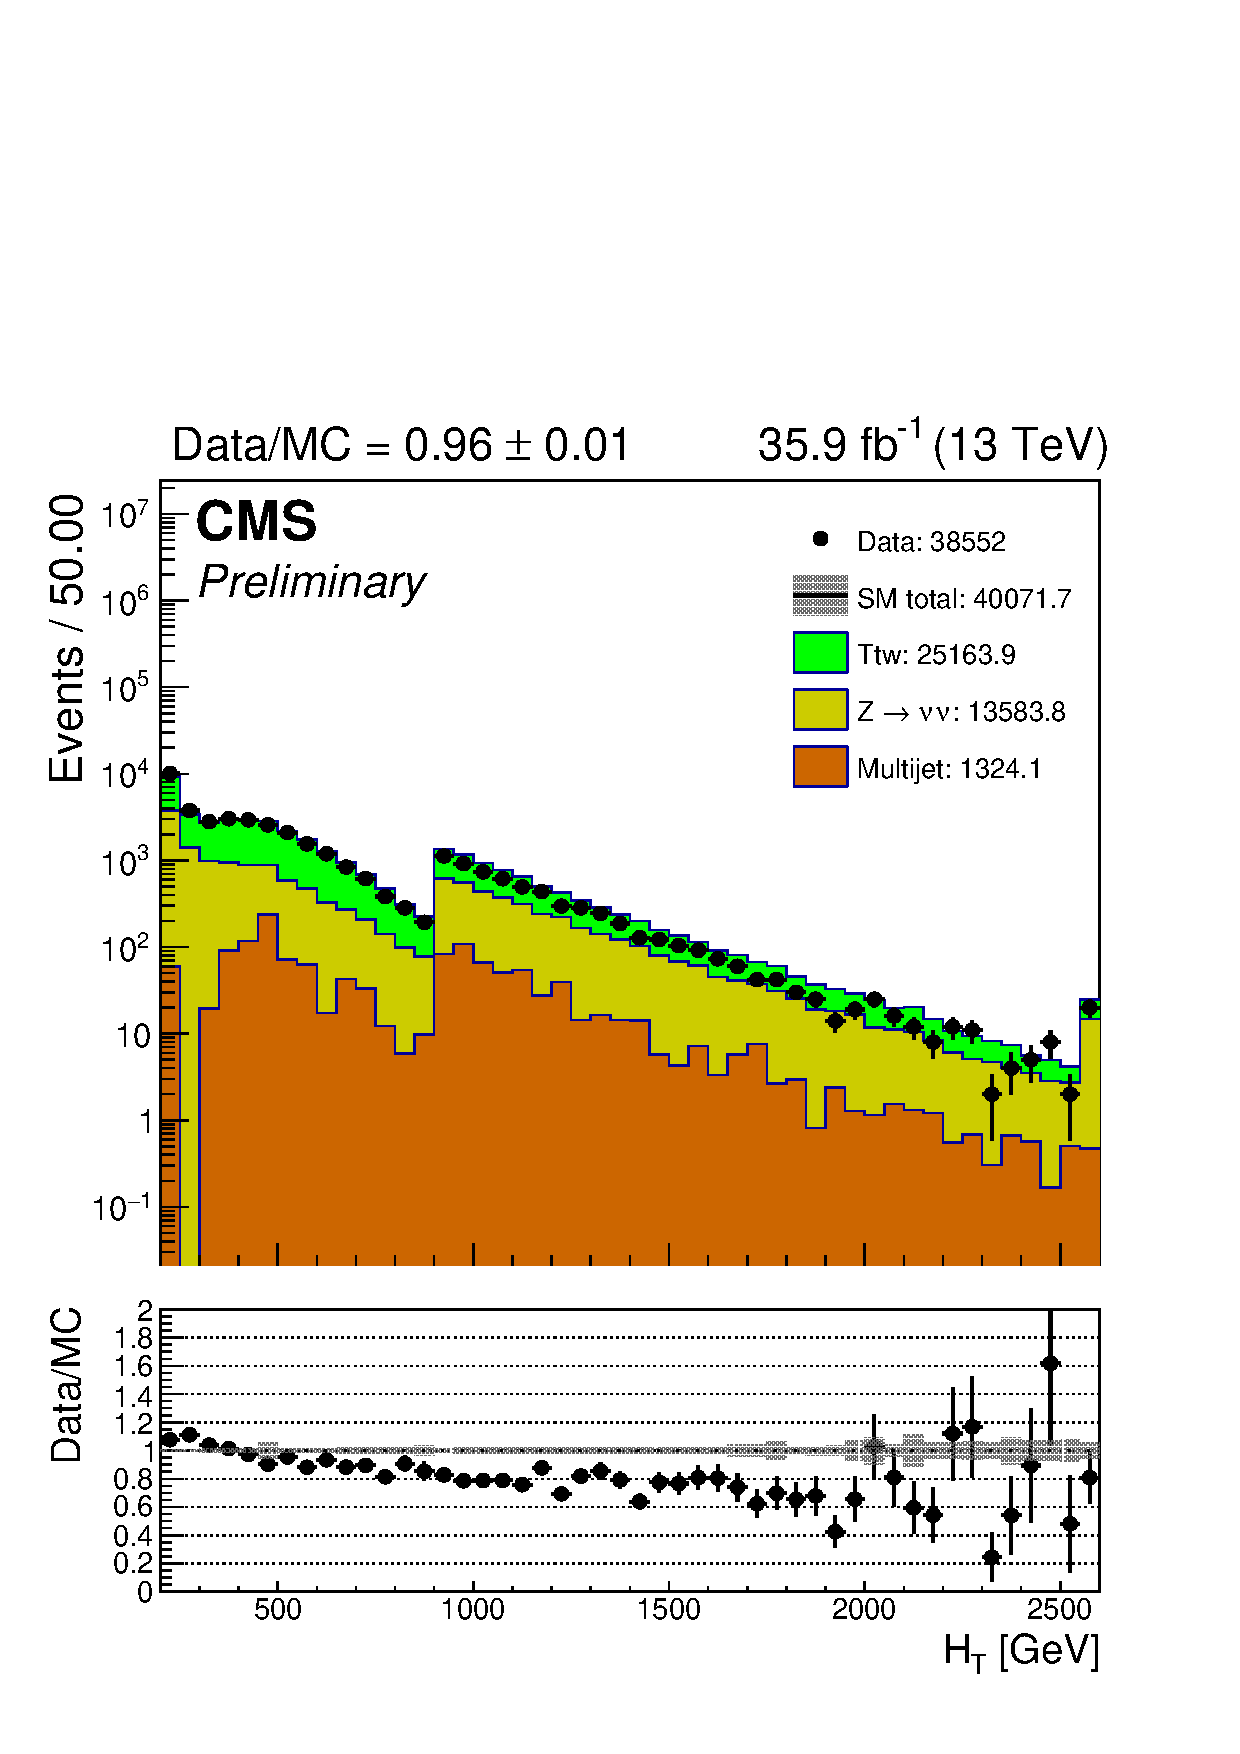
\includegraphics[width=0.5\textwidth]{figures/qcd/distributions/bdphisb_ht40}
  }
  \subfigure[Sideband \textbf{C} \njet distribution]{
    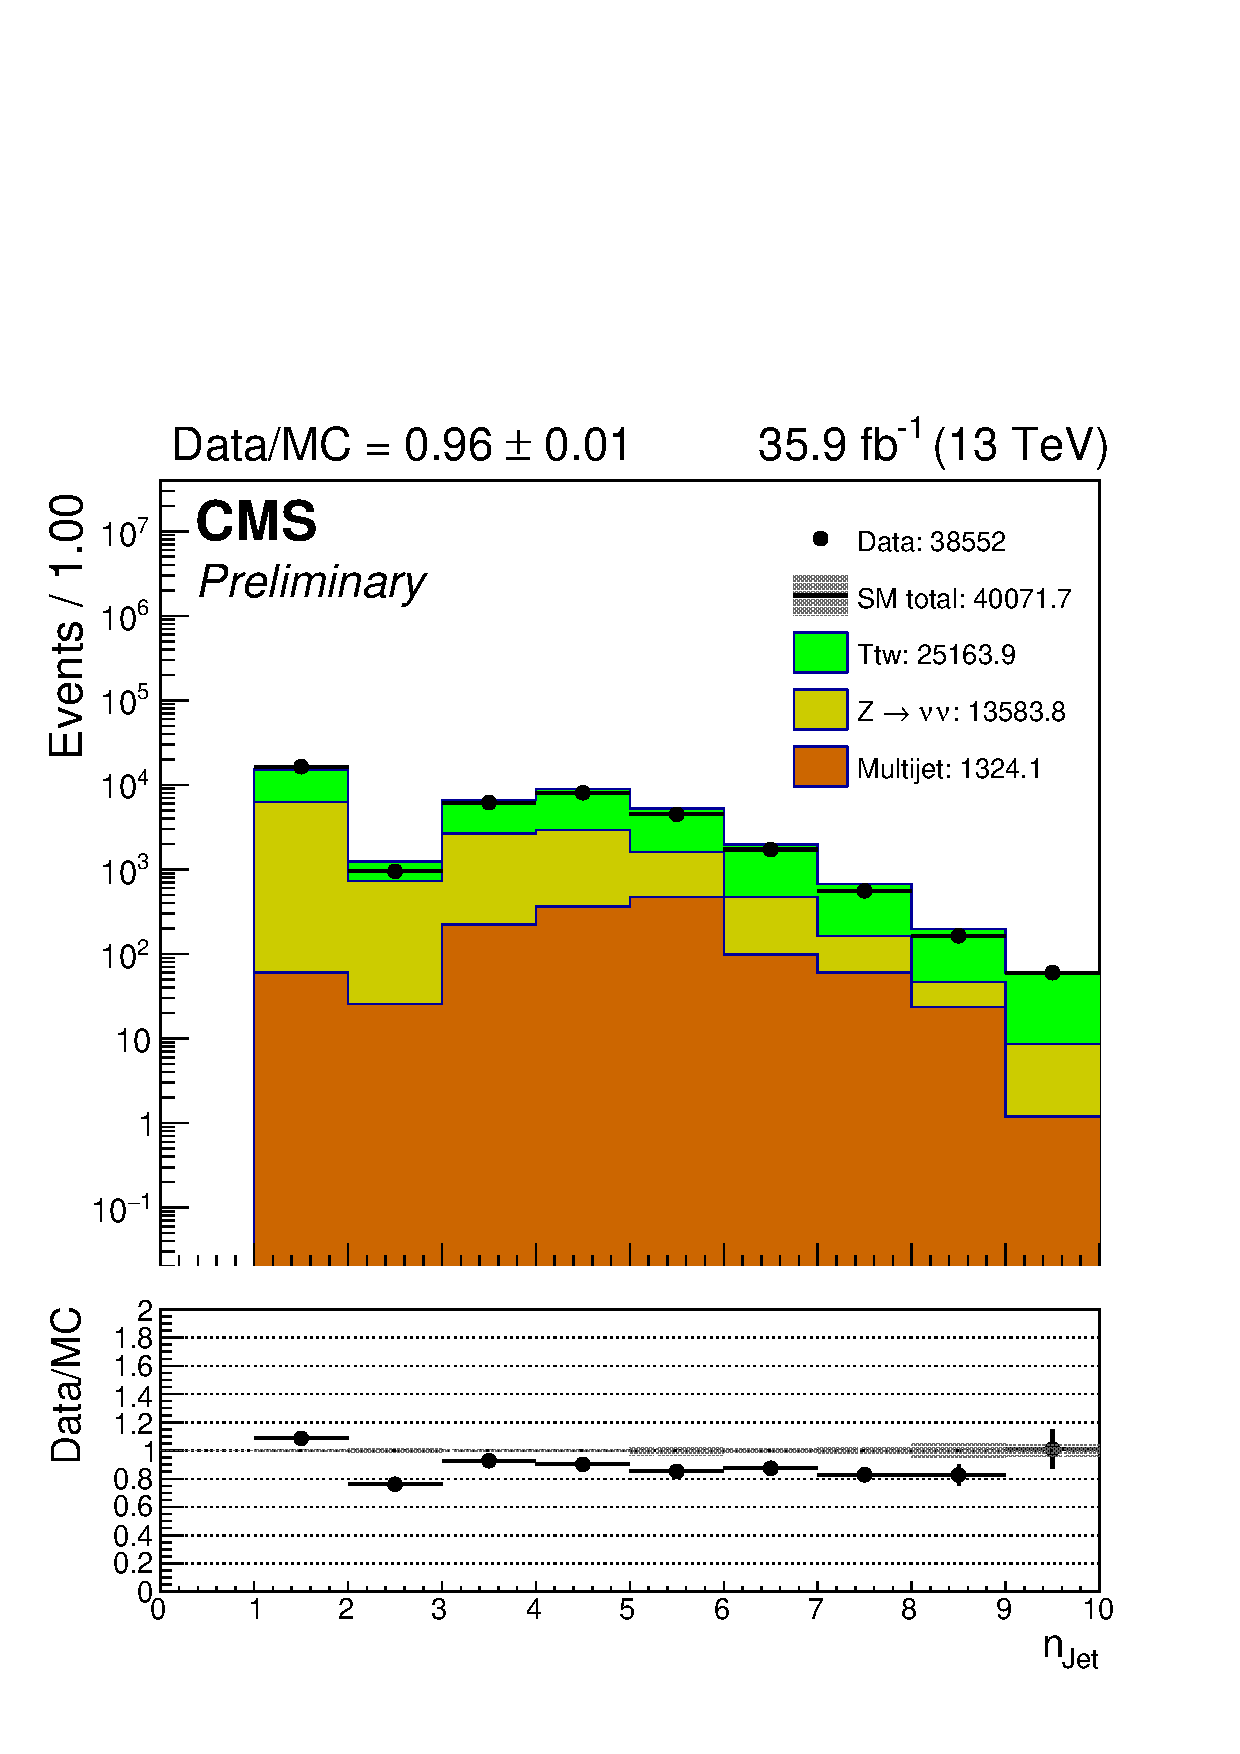
\includegraphics[width=0.5\textwidth]{figures/qcd/distributions/bdphisb_njet40}
  }
  \caption{Data and (uncorrected) MC comparisons of the \scalht and \njet
    distributions in the sidebands \textbf{B} and \textbf{C}.}
  \label{fig:qcd_distributions_1}
\end{figure}

\begin{figure}[!h]
  \subfigure[Sideband \textbf{A} \scalht distribution]{
    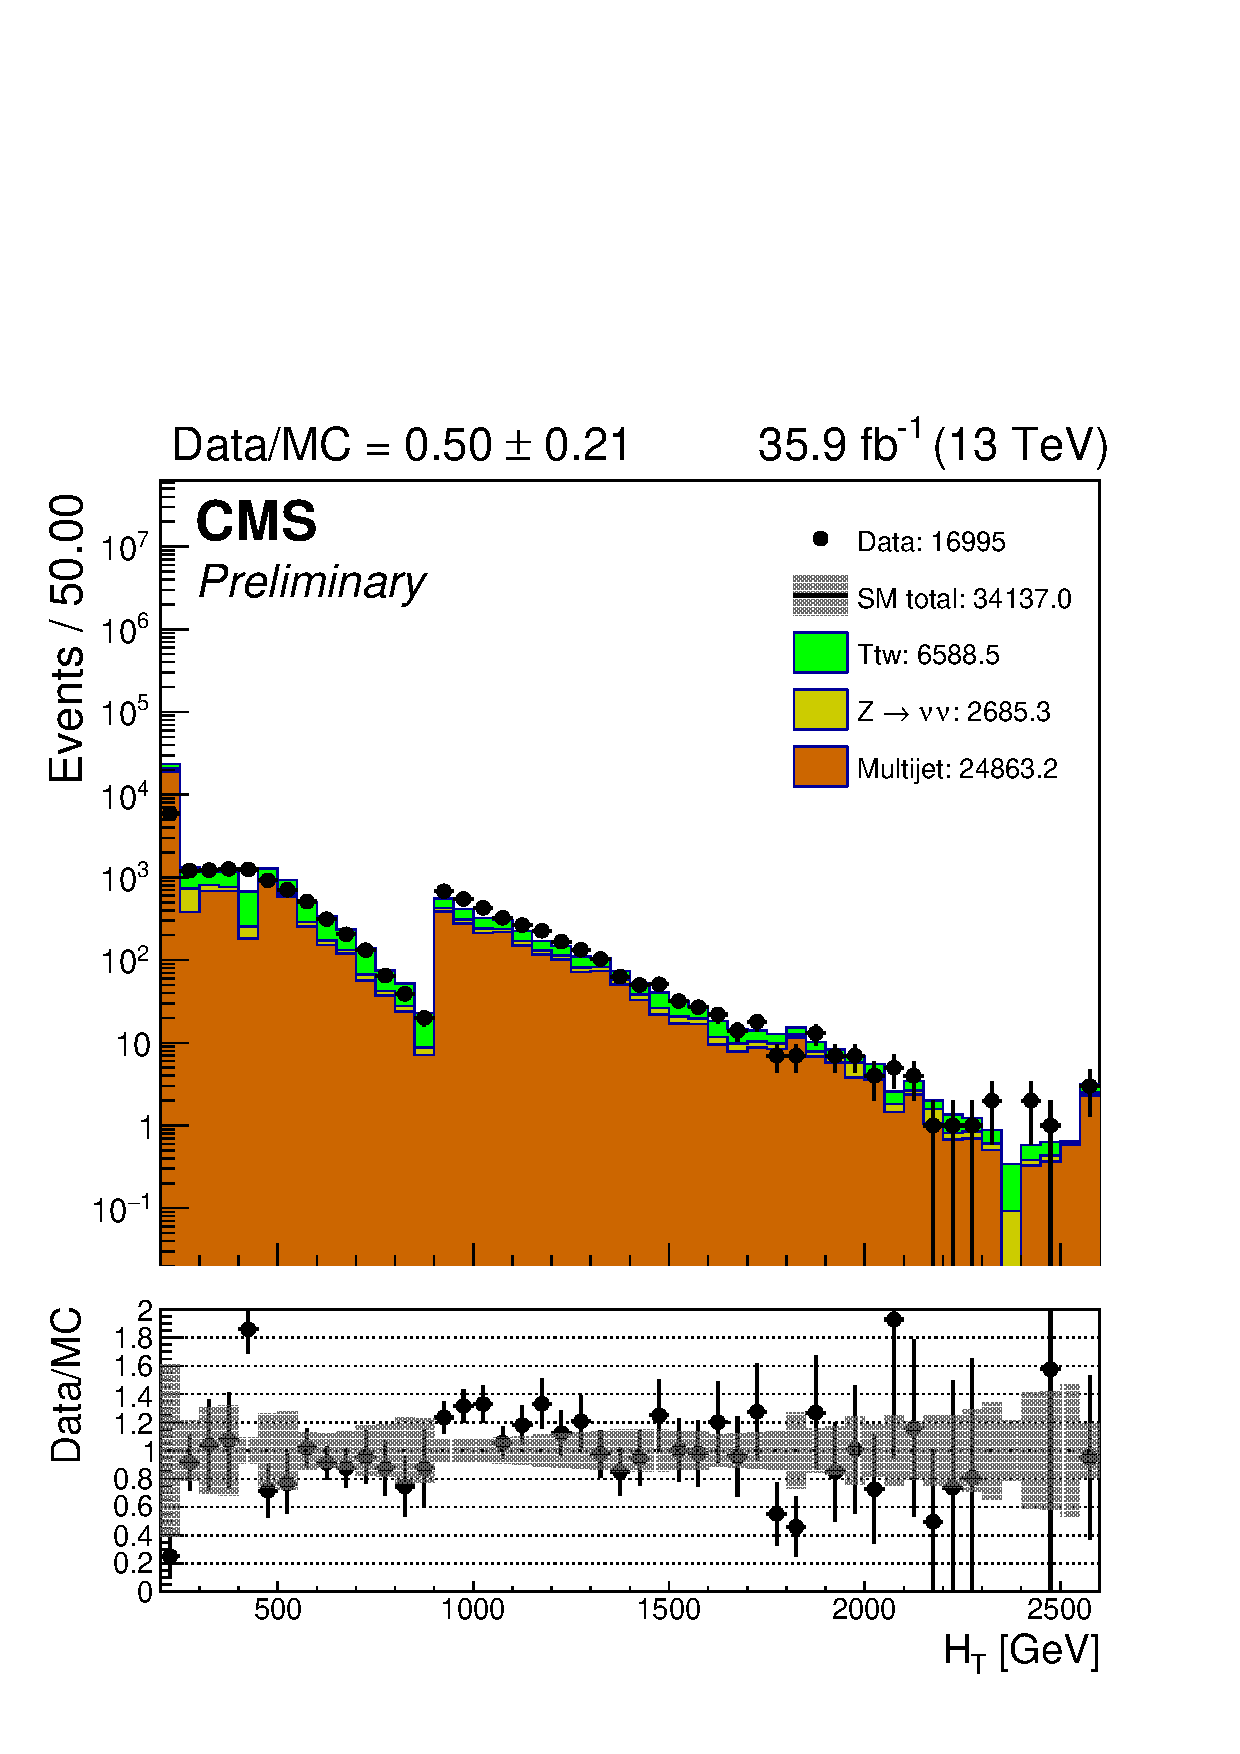
\includegraphics[width=0.5\textwidth]{figures/qcd/distributions/doublesb_ht40}
  }
  \subfigure[Sideband \textbf{A} \njet distribution]{
    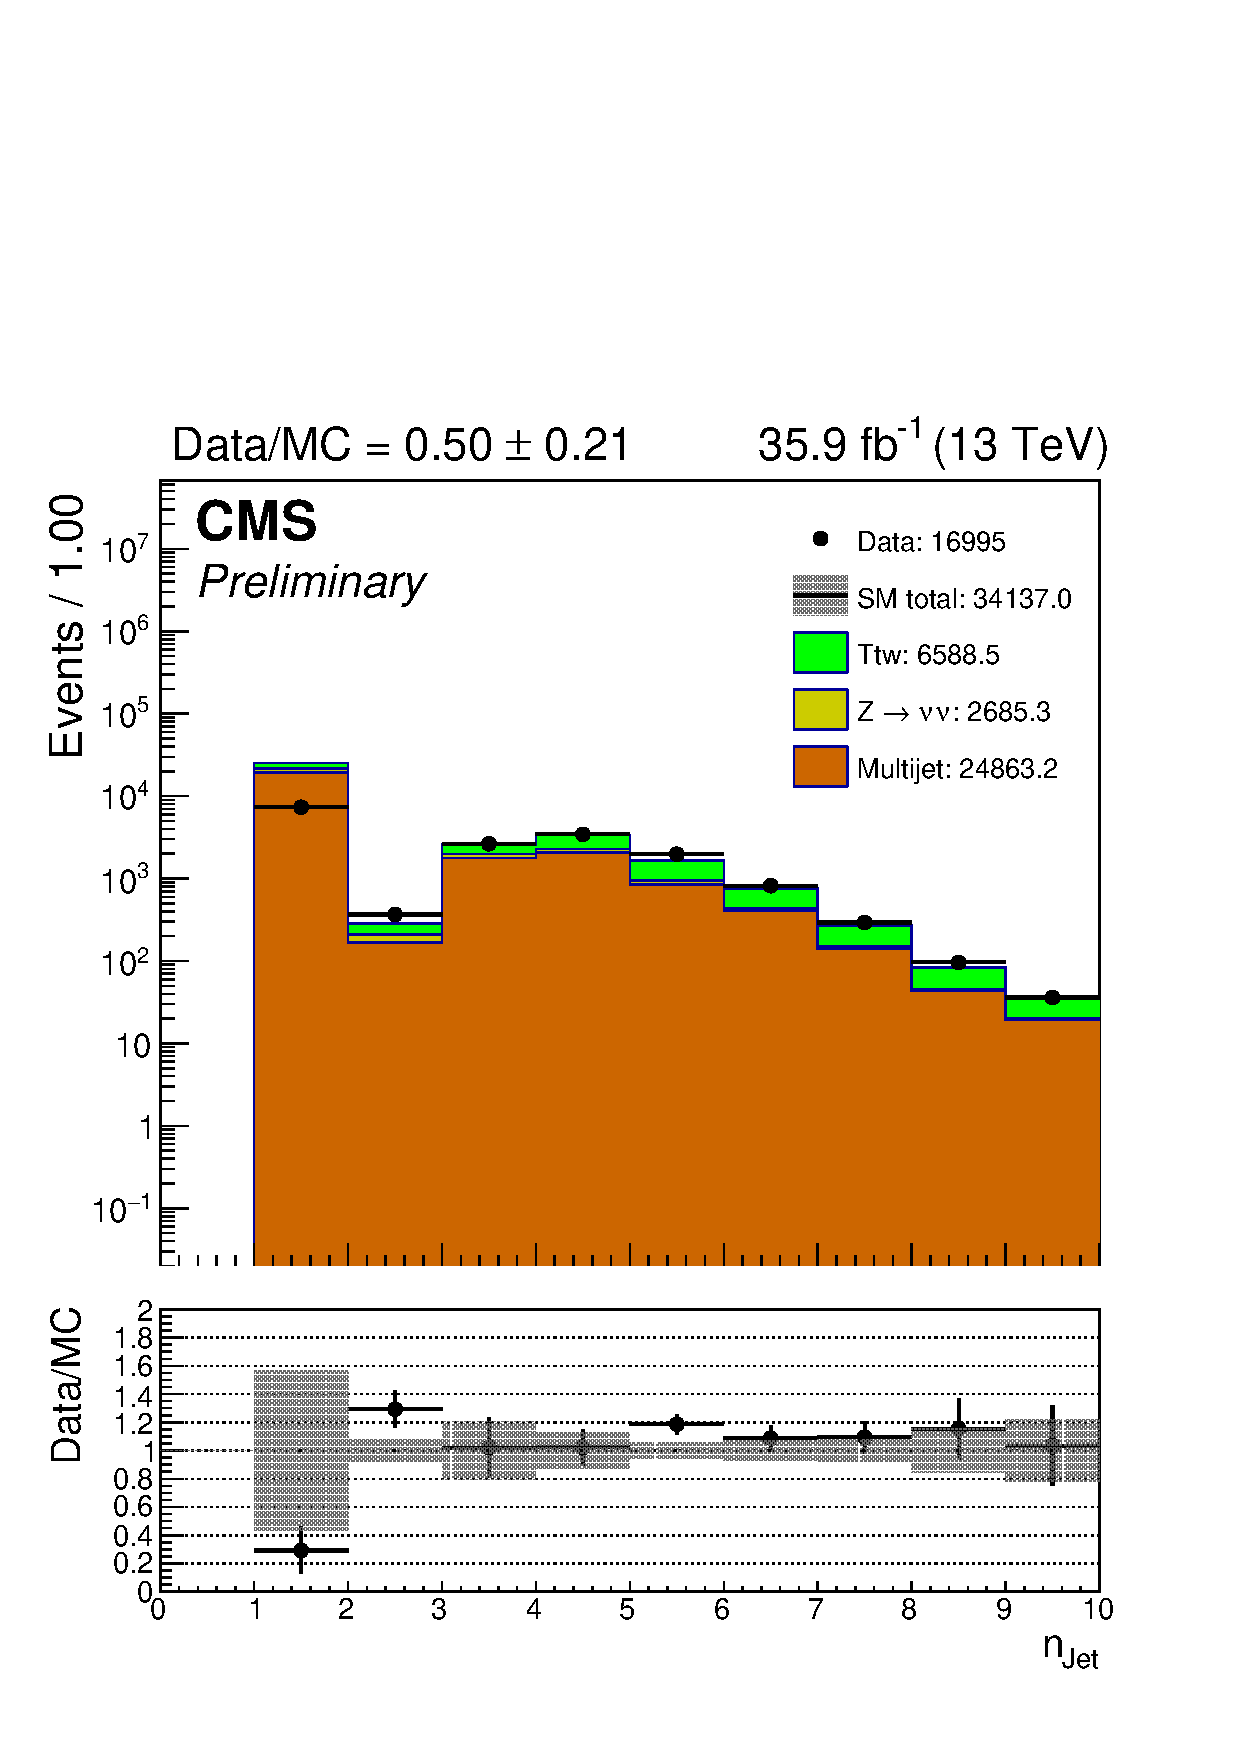
\includegraphics[width=0.5\textwidth]{figures/qcd/distributions/doublesb_njet40}
  }
  \caption{Data and (uncorrected) MC comparisons of the \scalht and \njet
      distributions in the sideband \text{A}.}
  \label{fig:qcd_distributions_2}
\end{figure}

\clearpage
\begin{figure}[!h]
    \centering
    \subfigure[$200<\scalht<250$ \gev]{
        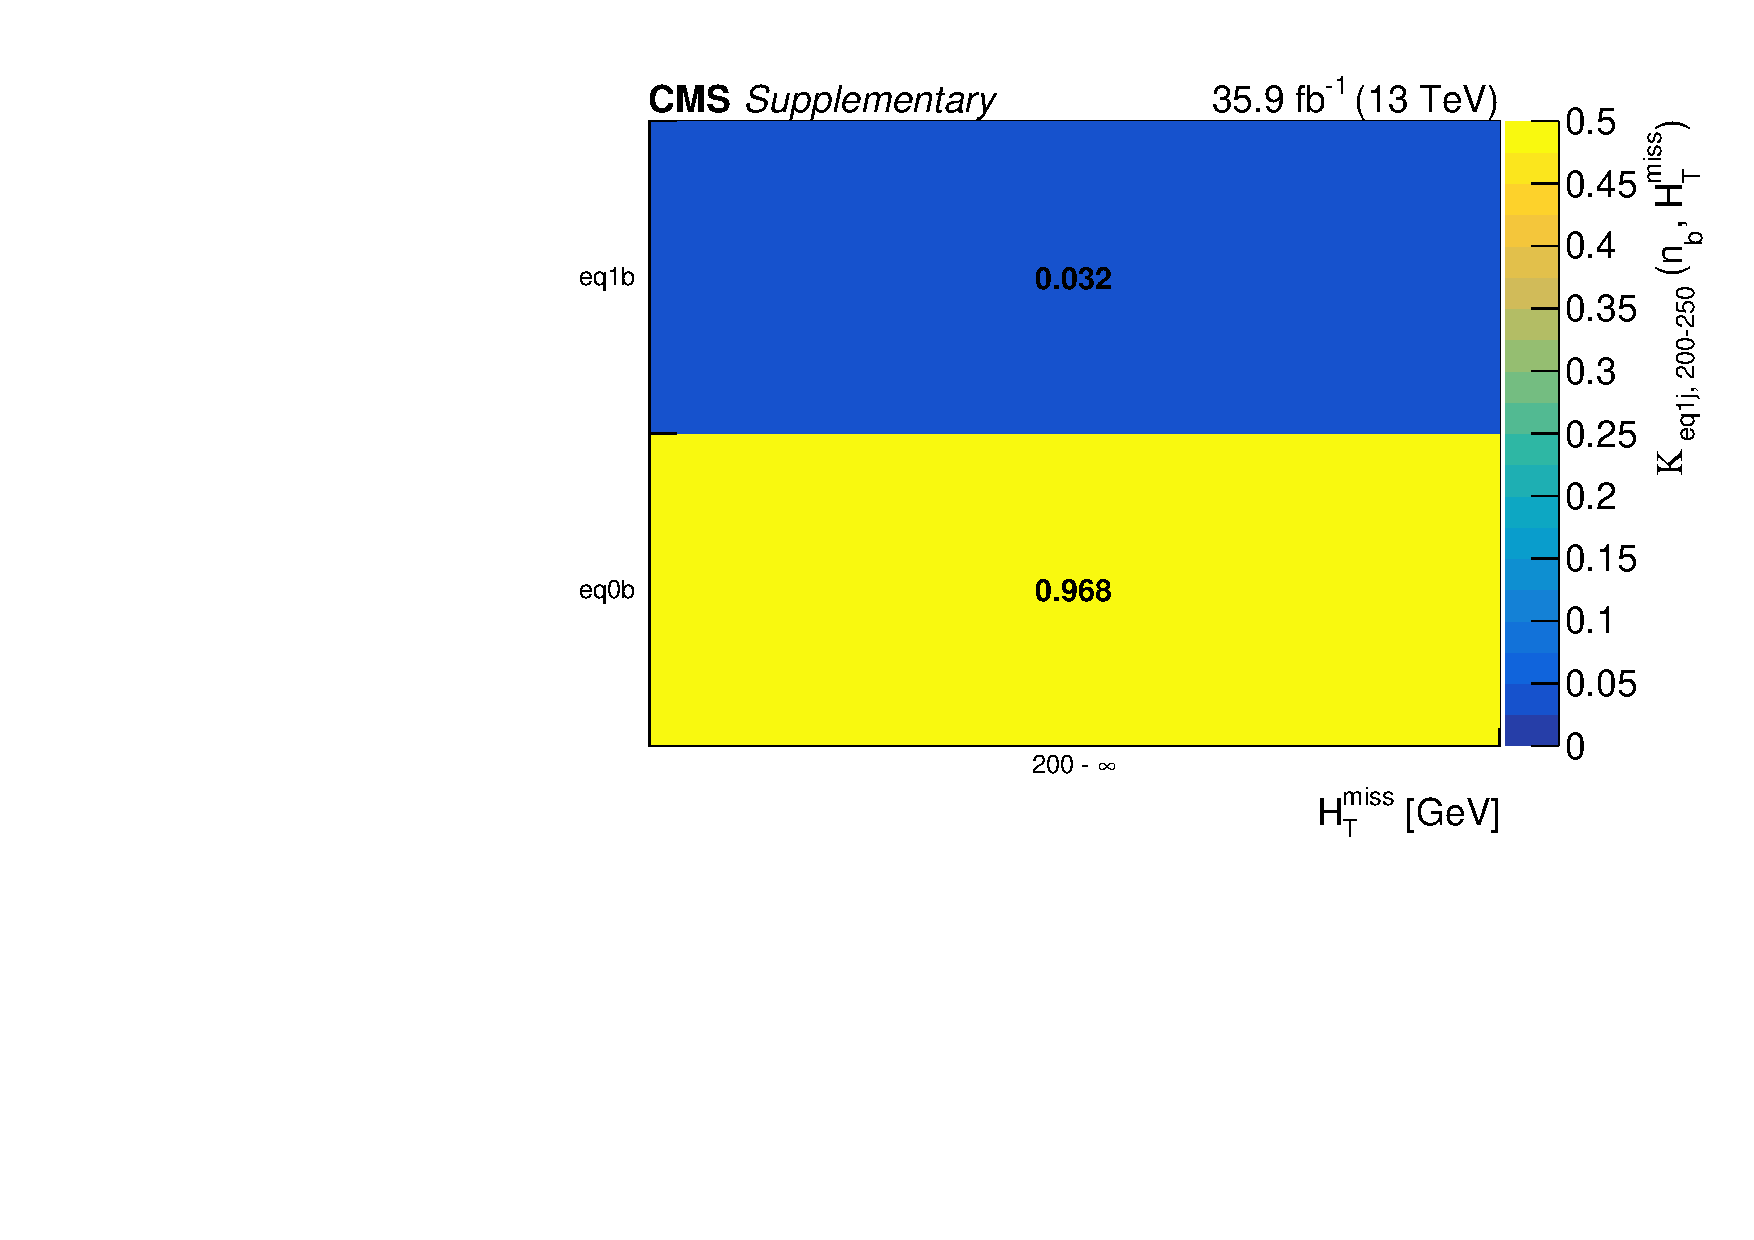
\includegraphics[width=0.3\textwidth]{figures/qcd/ewk_kappas/ewkKappa_eq1j_200-250}
    } ~~
    \subfigure[$250<\scalht<300$ \gev]{
        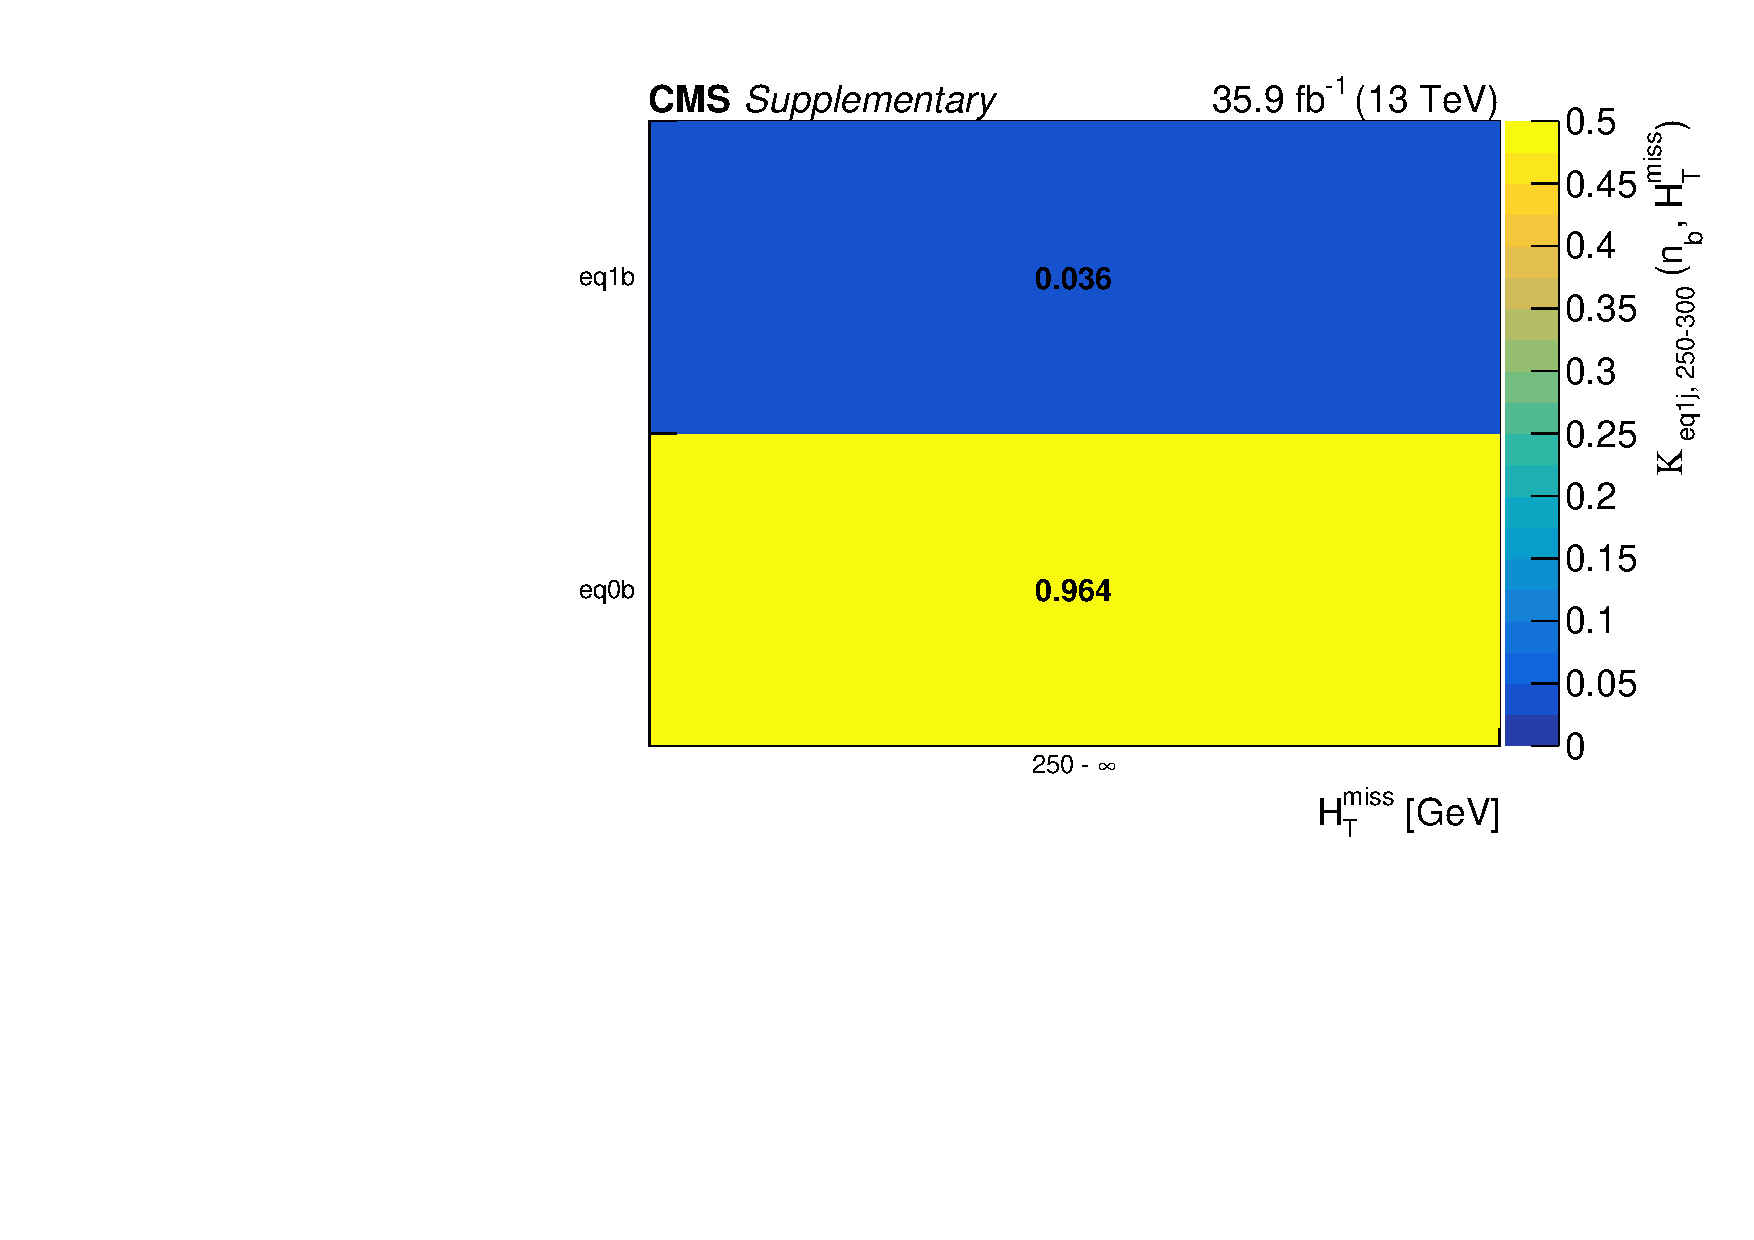
\includegraphics[width=0.3\textwidth]{figures/qcd/ewk_kappas/ewkKappa_eq1j_250-300}
    } ~~
    \subfigure[$300<\scalht<350$ \gev]{
        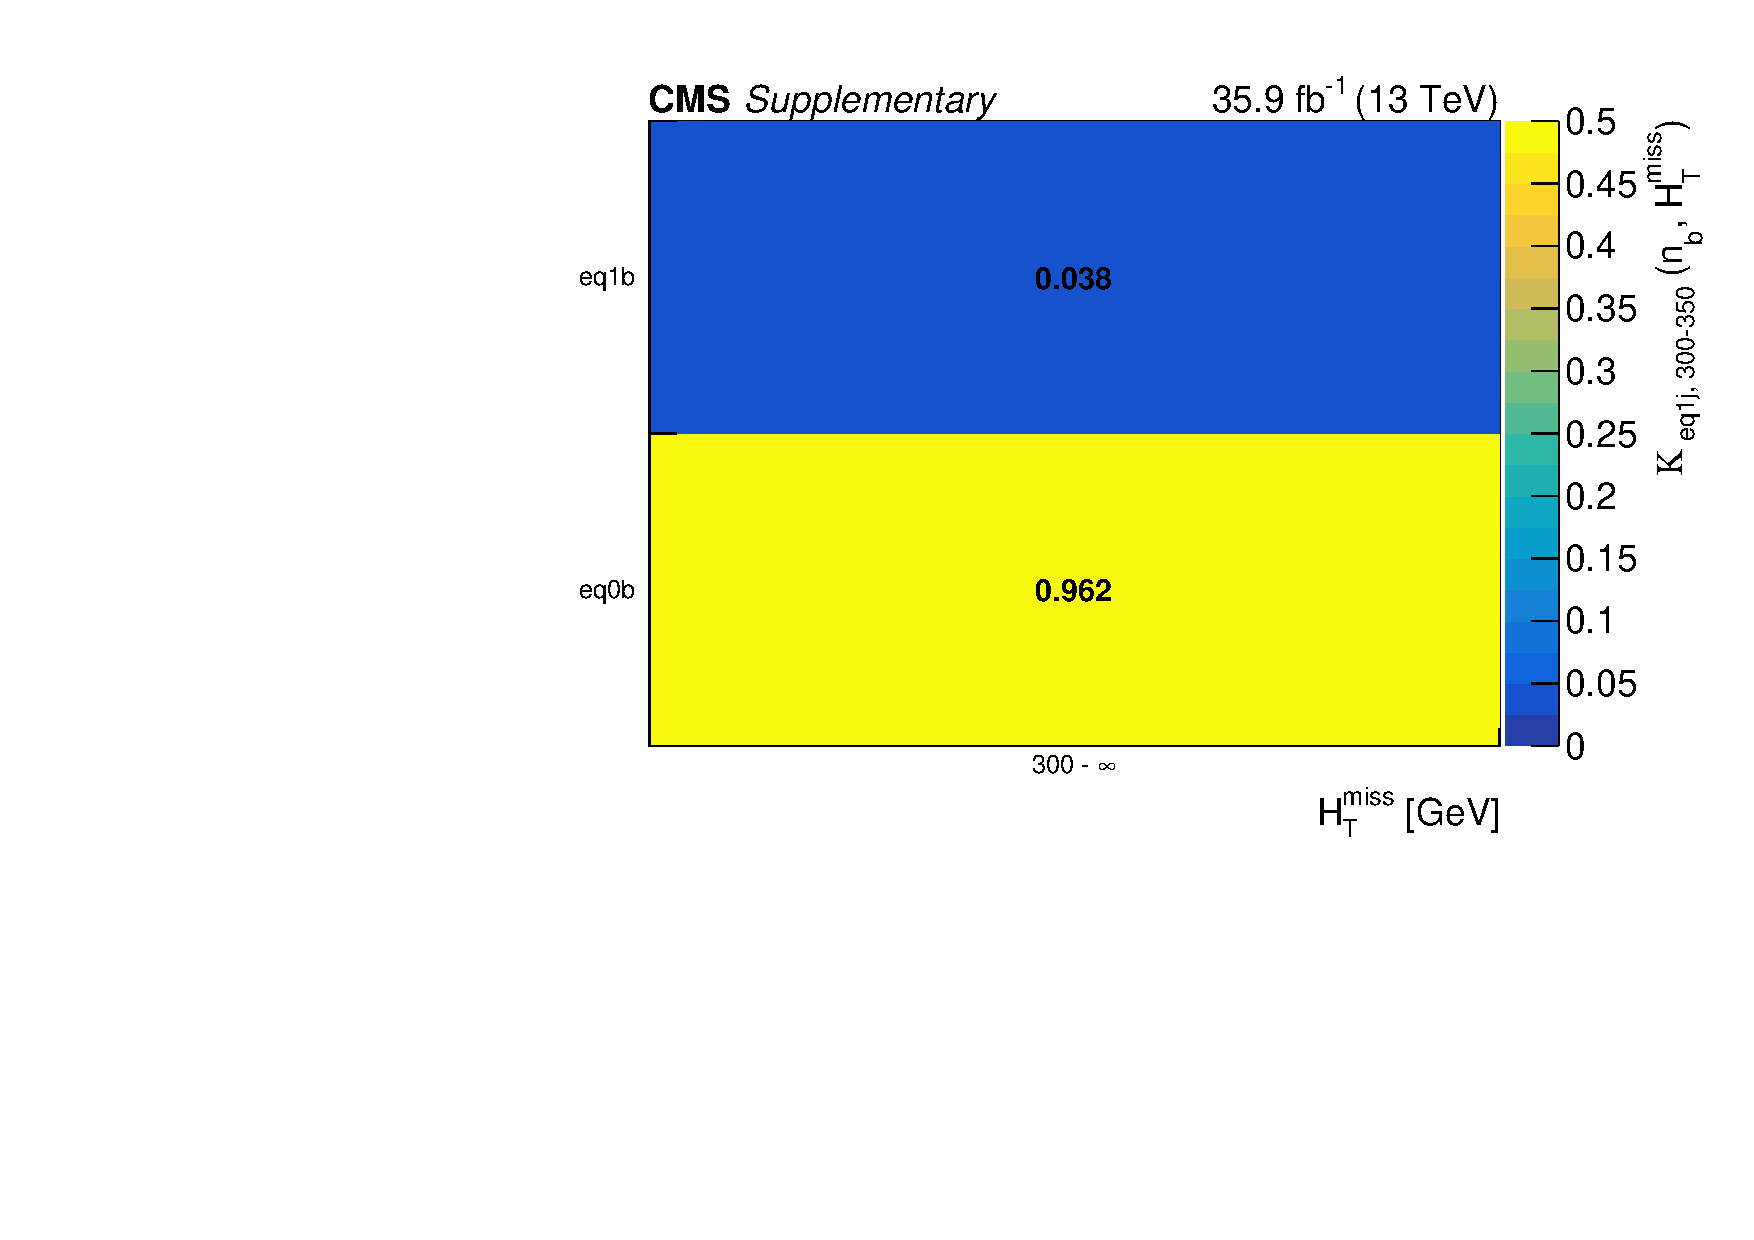
\includegraphics[width=0.3\textwidth]{figures/qcd/ewk_kappas/ewkKappa_eq1j_300-350}
    } \\
    \subfigure[$350<\scalht<400$ \gev]{
        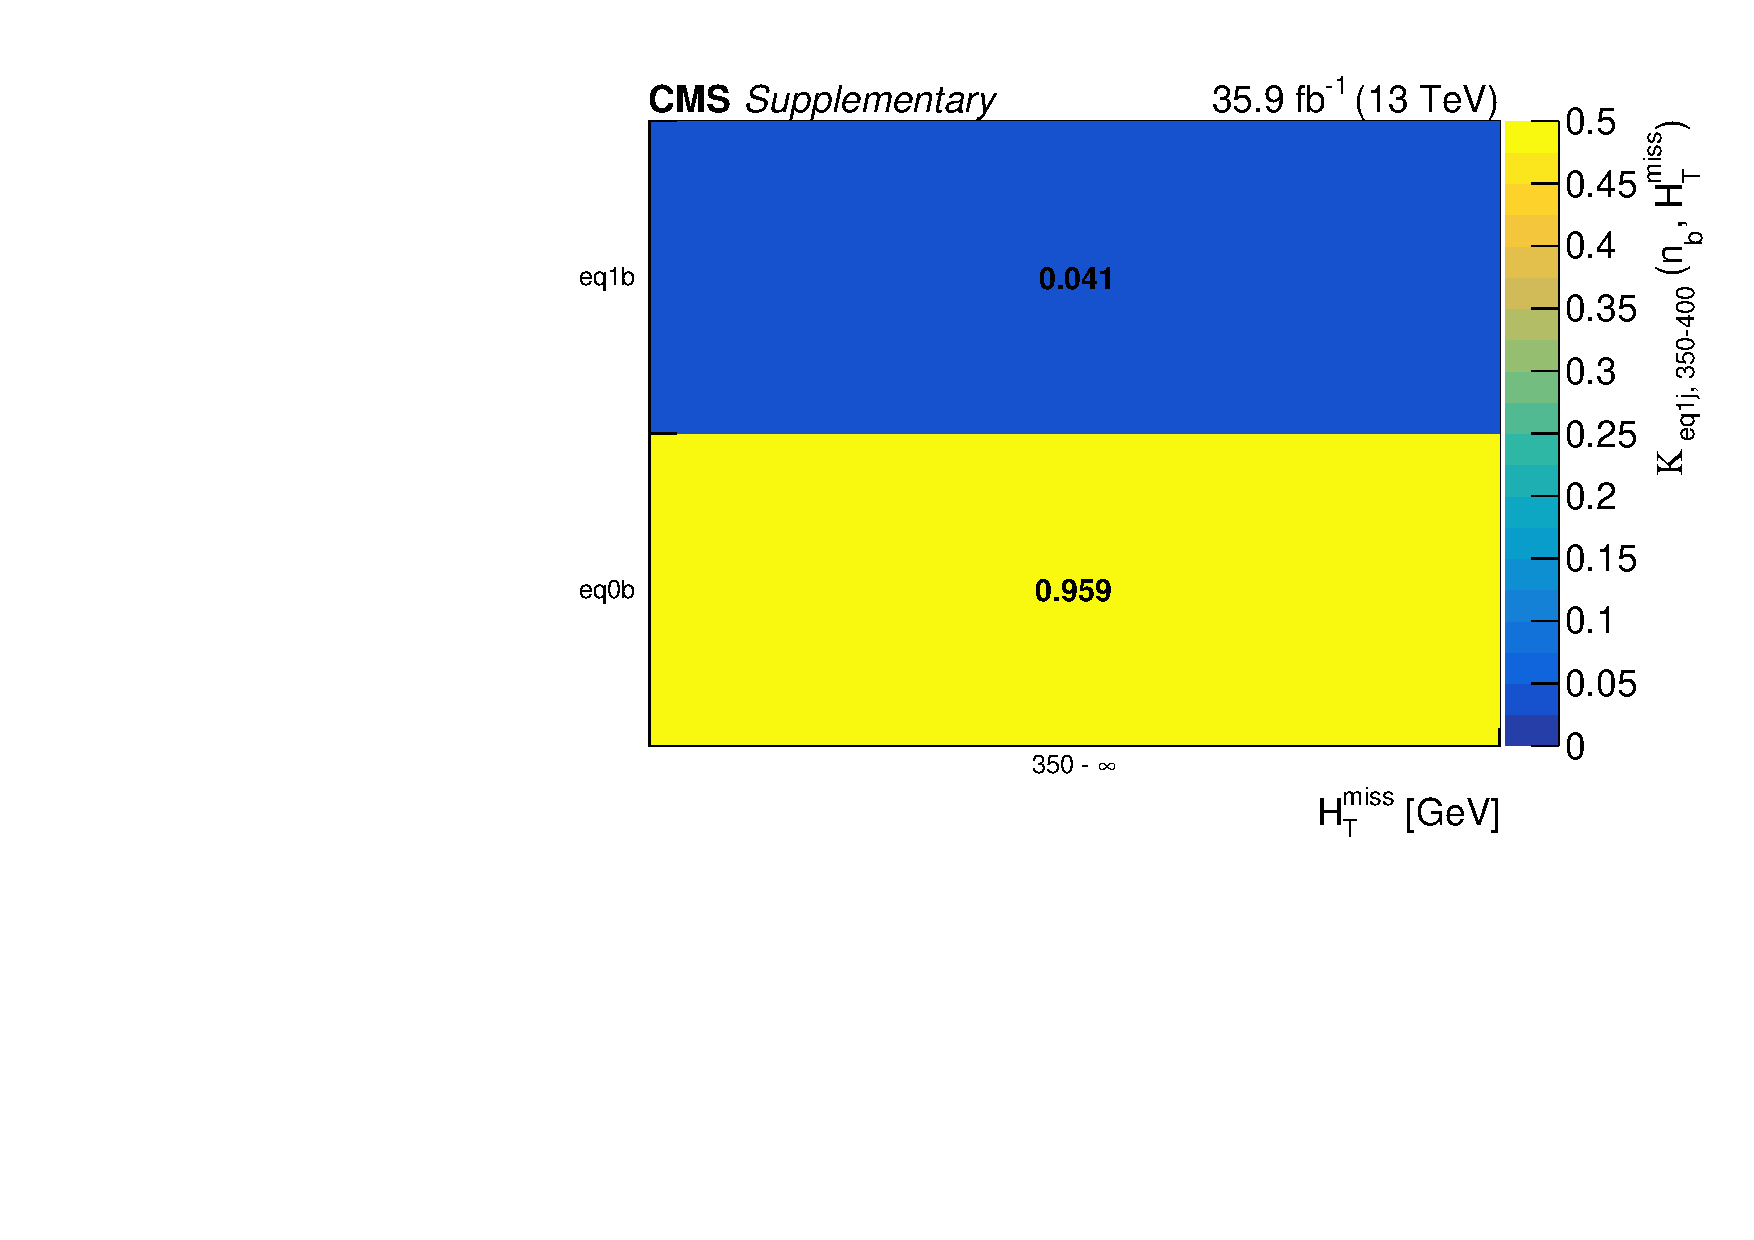
\includegraphics[width=0.3\textwidth]{figures/qcd/ewk_kappas/ewkKappa_eq1j_350-400}
    } ~~
    \subfigure[$400<\scalht<500$ \gev]{
        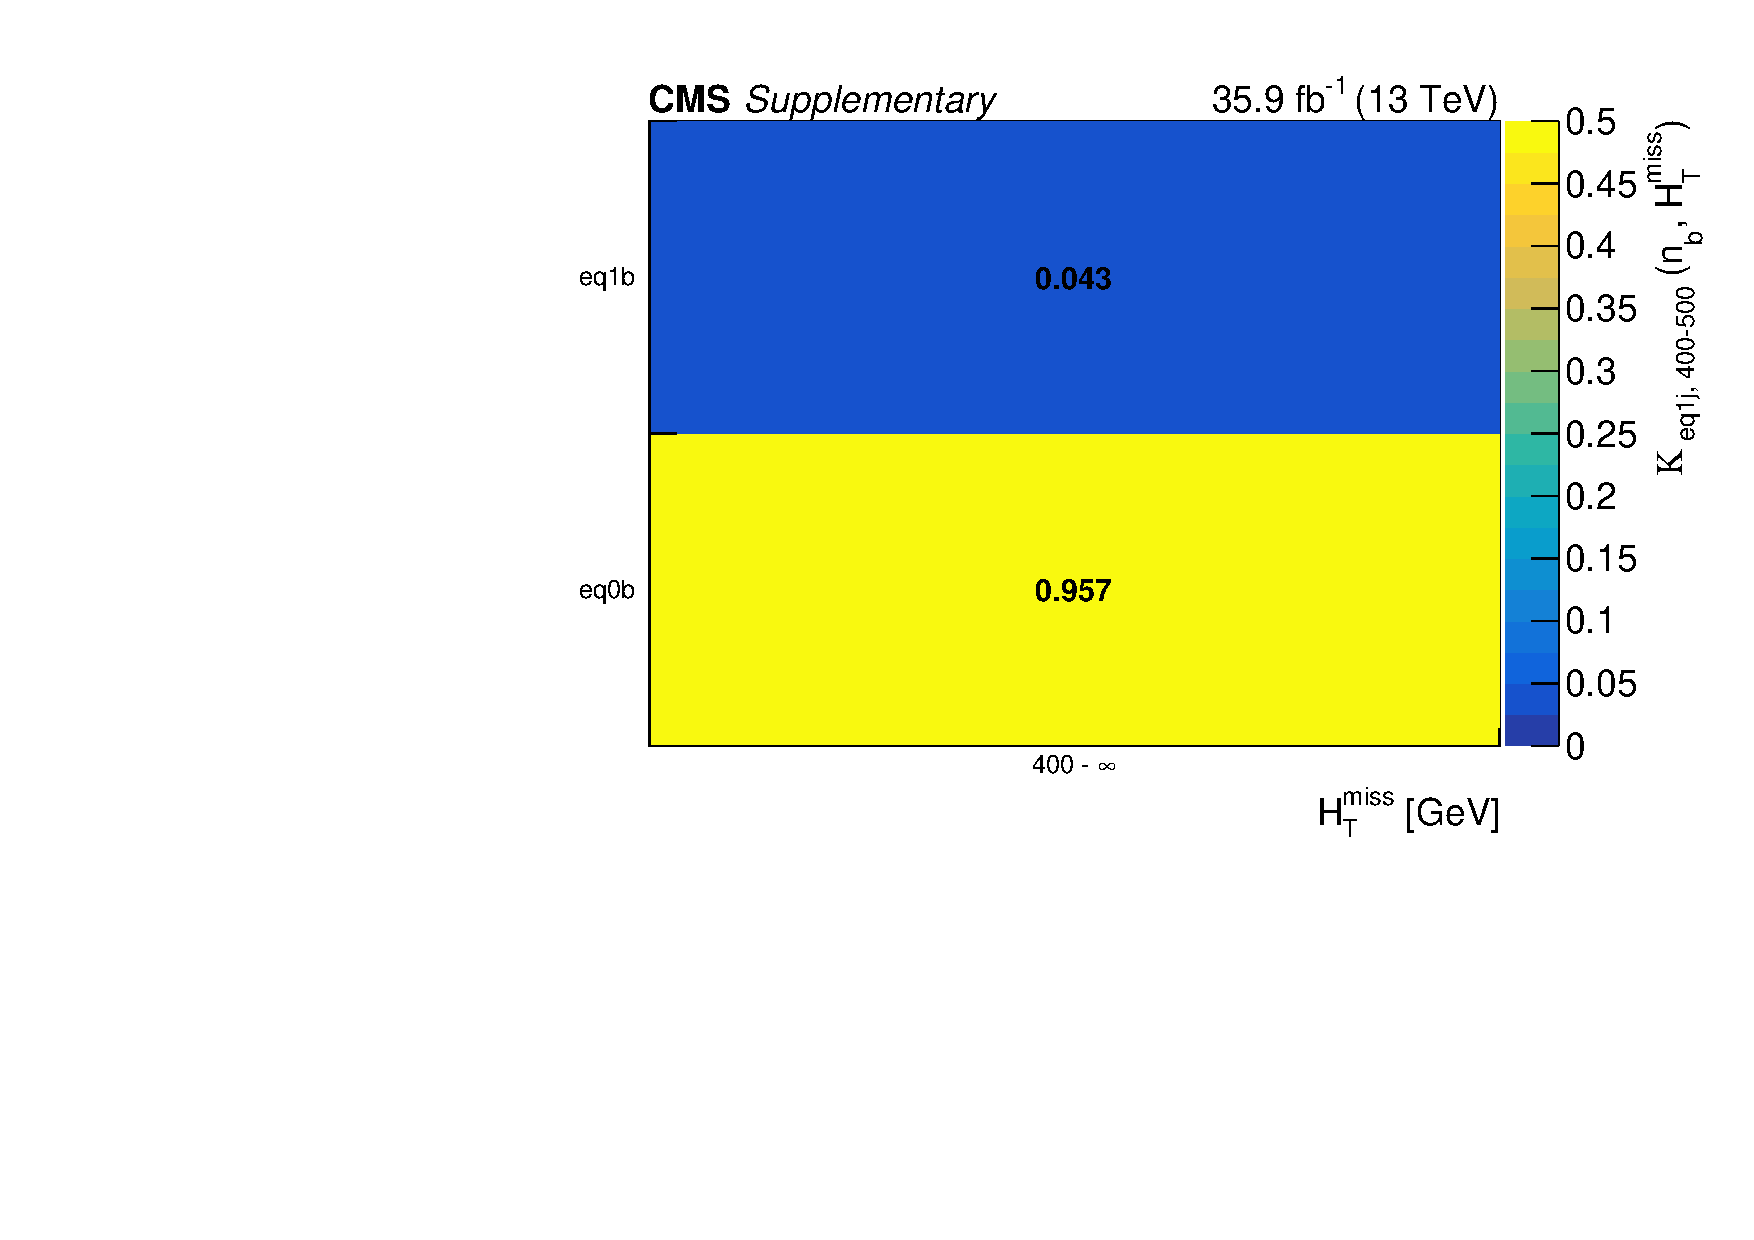
\includegraphics[width=0.3\textwidth]{figures/qcd/ewk_kappas/ewkKappa_eq1j_400-500}
    } ~~
    \subfigure[$500<\scalht<600$ \gev]{
        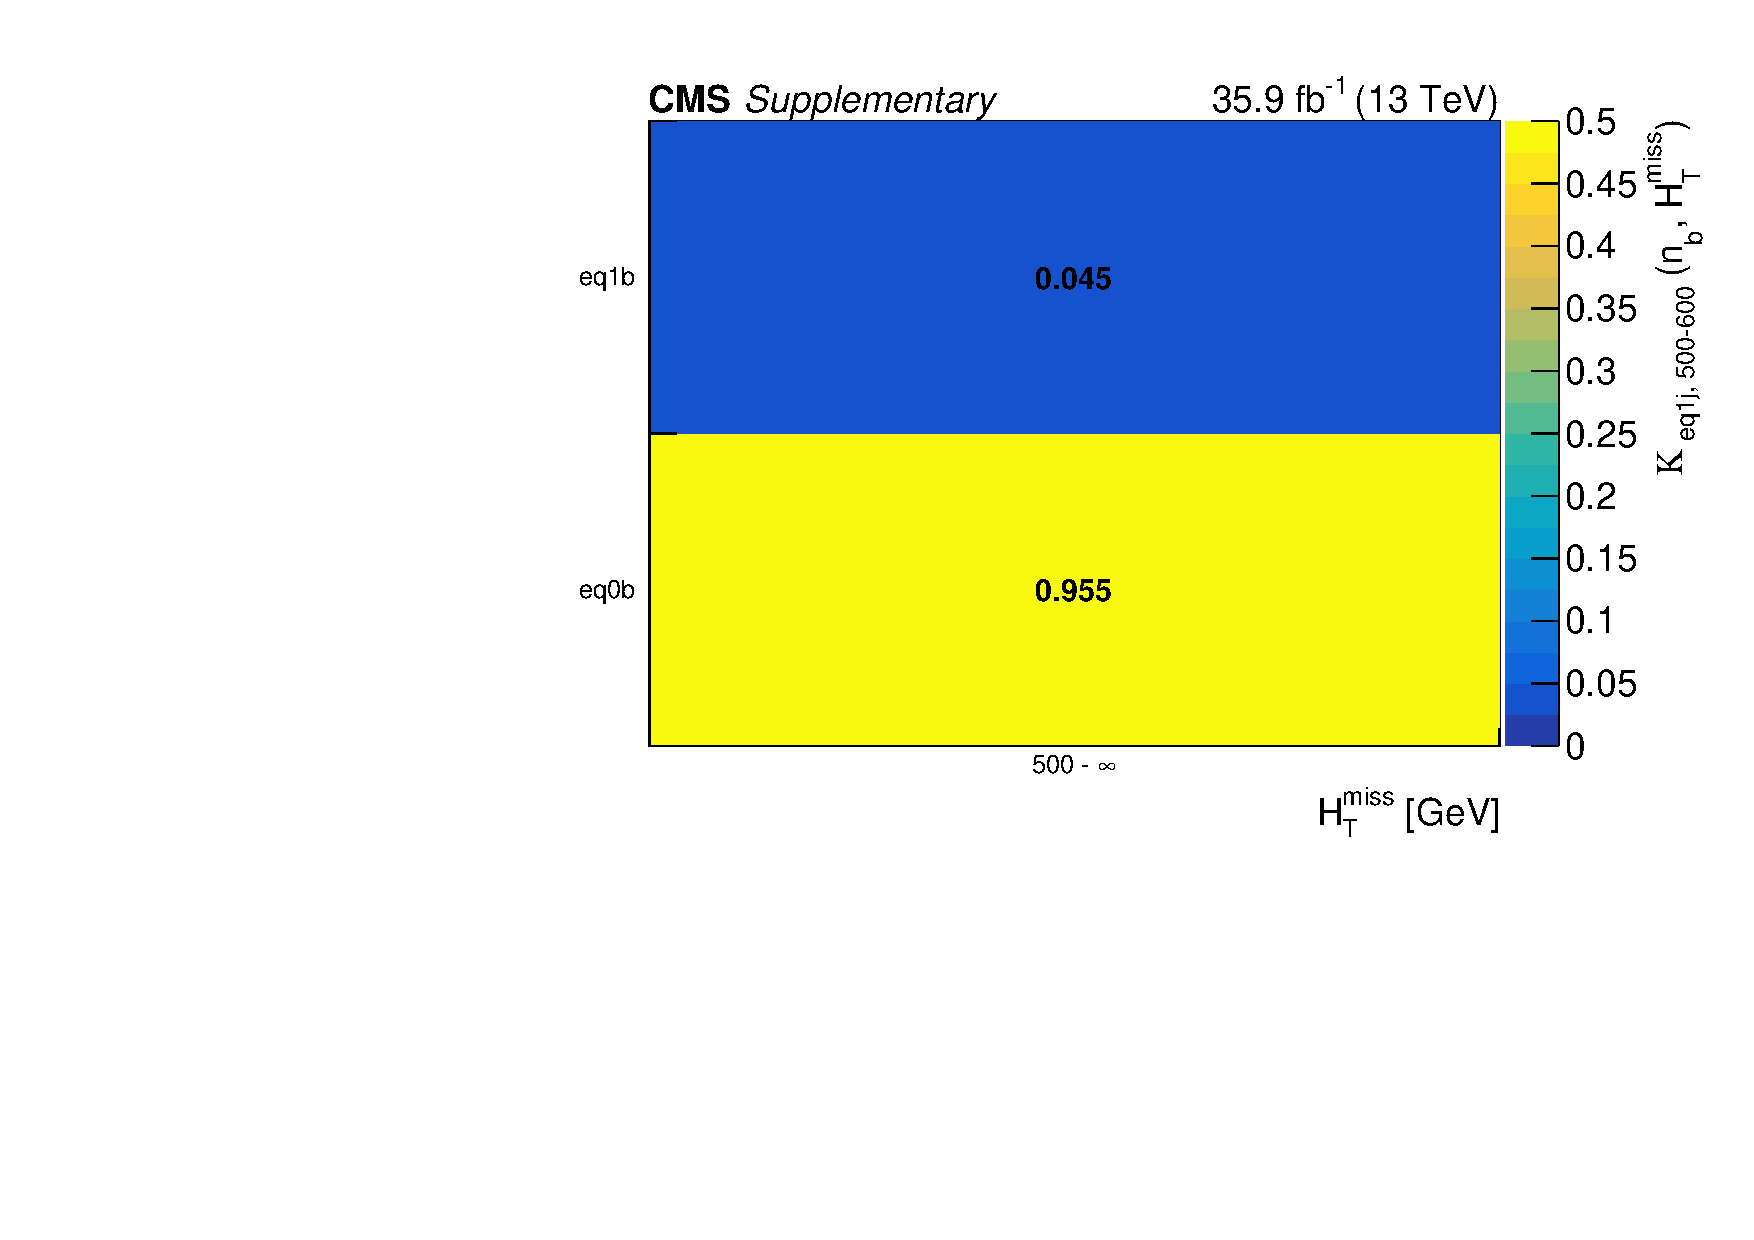
\includegraphics[width=0.3\textwidth]{figures/qcd/ewk_kappas/ewkKappa_eq1j_500-600}
    } \\
    \subfigure[$600<\scalht<750$ \gev]{
        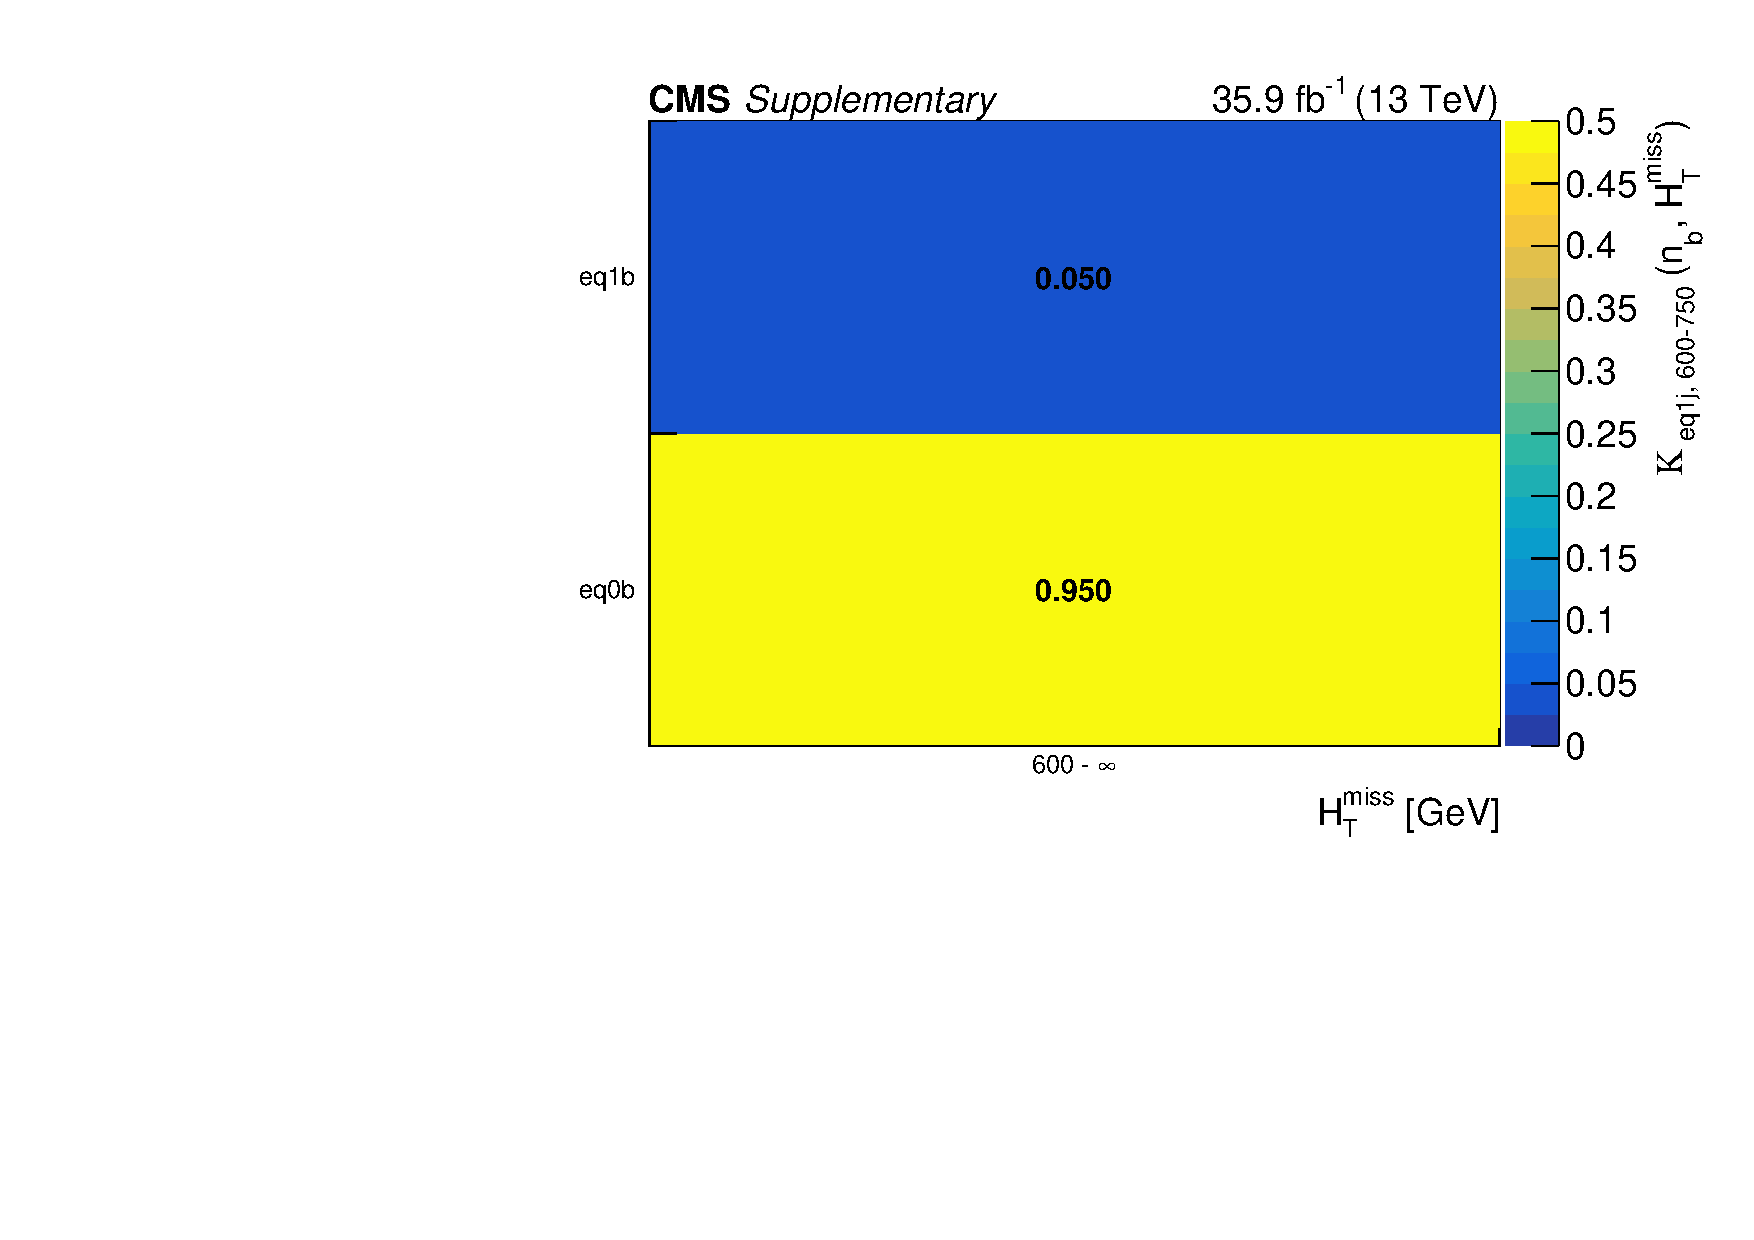
\includegraphics[width=0.3\textwidth]{figures/qcd/ewk_kappas/ewkKappa_eq1j_600-750}
    } ~~
    \subfigure[$750<\scalht<900$ \gev]{
        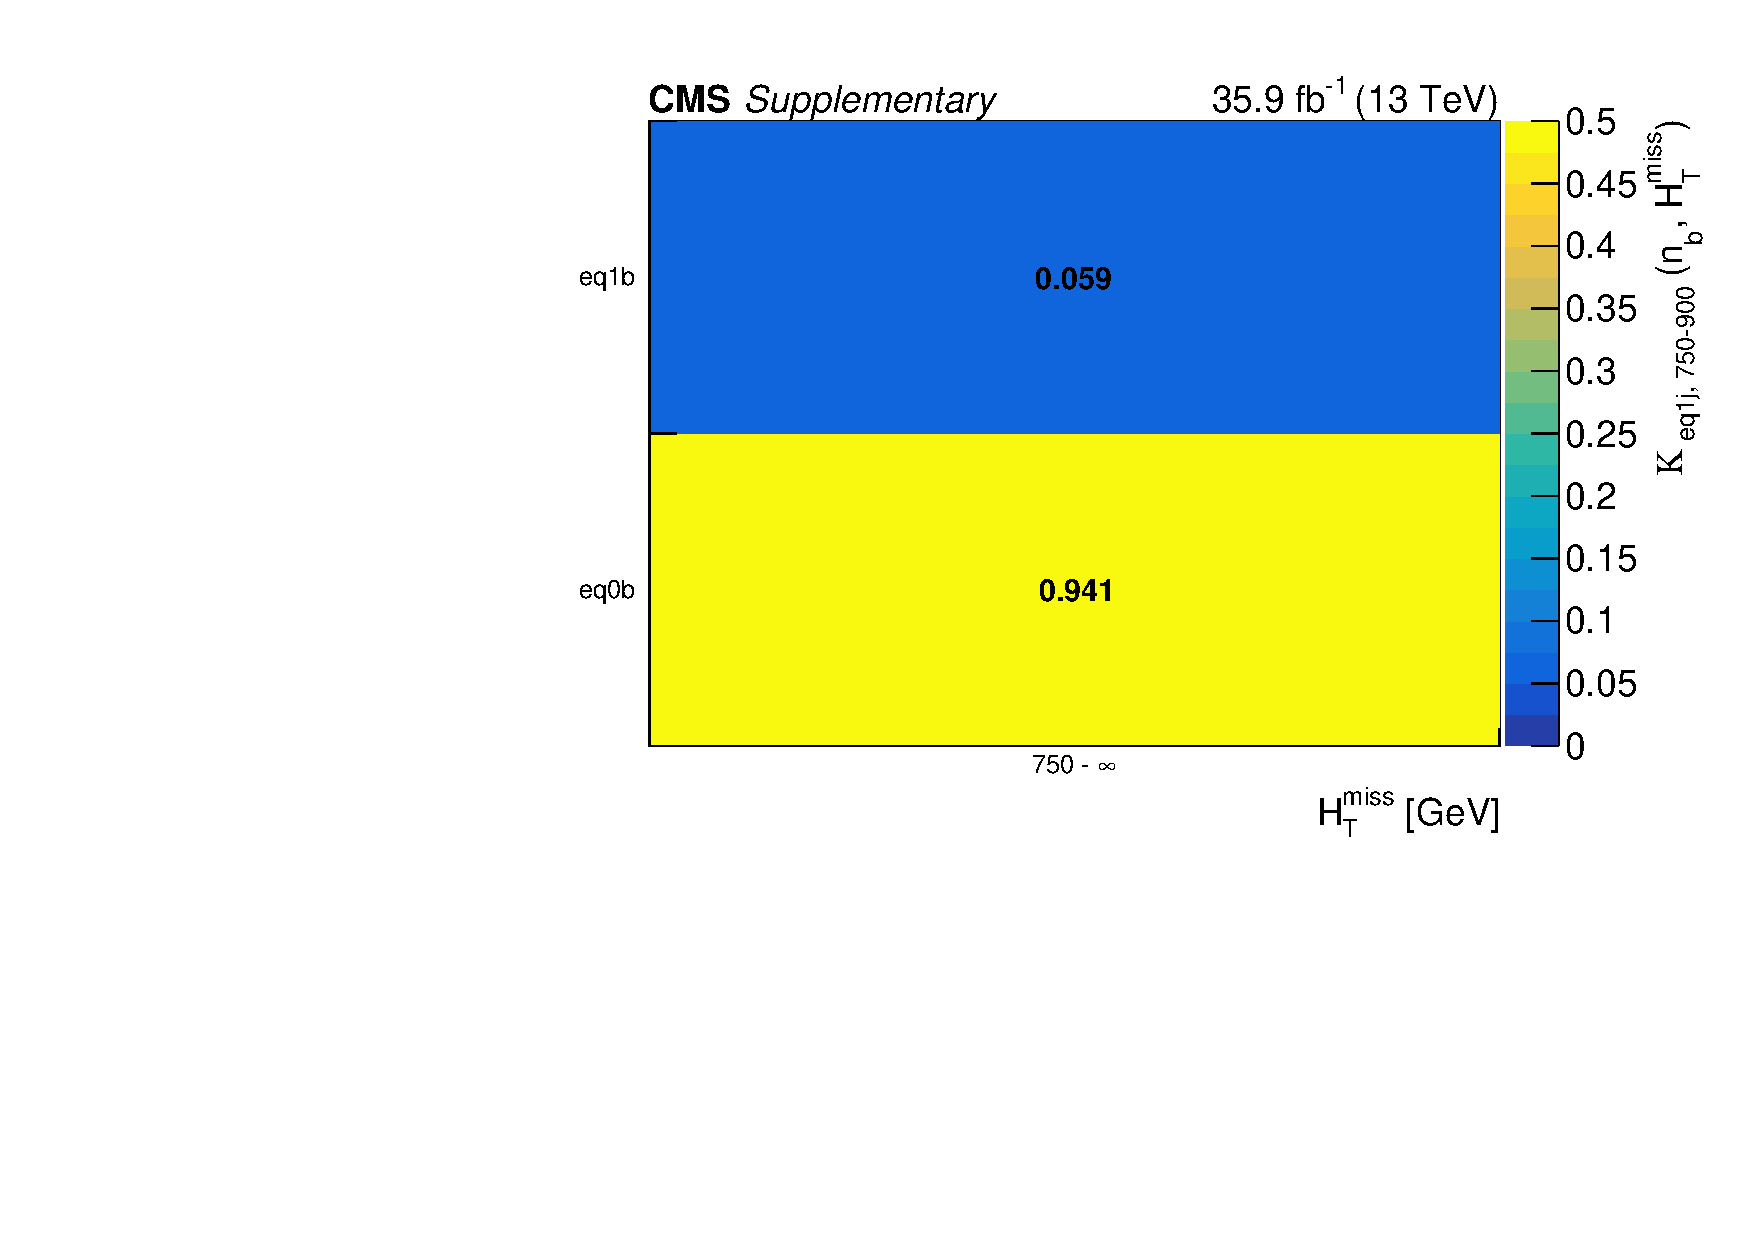
\includegraphics[width=0.3\textwidth]{figures/qcd/ewk_kappas/ewkKappa_eq1j_750-900}
    } ~~
    \subfigure[$900<\scalht<\infty$ \gev]{
        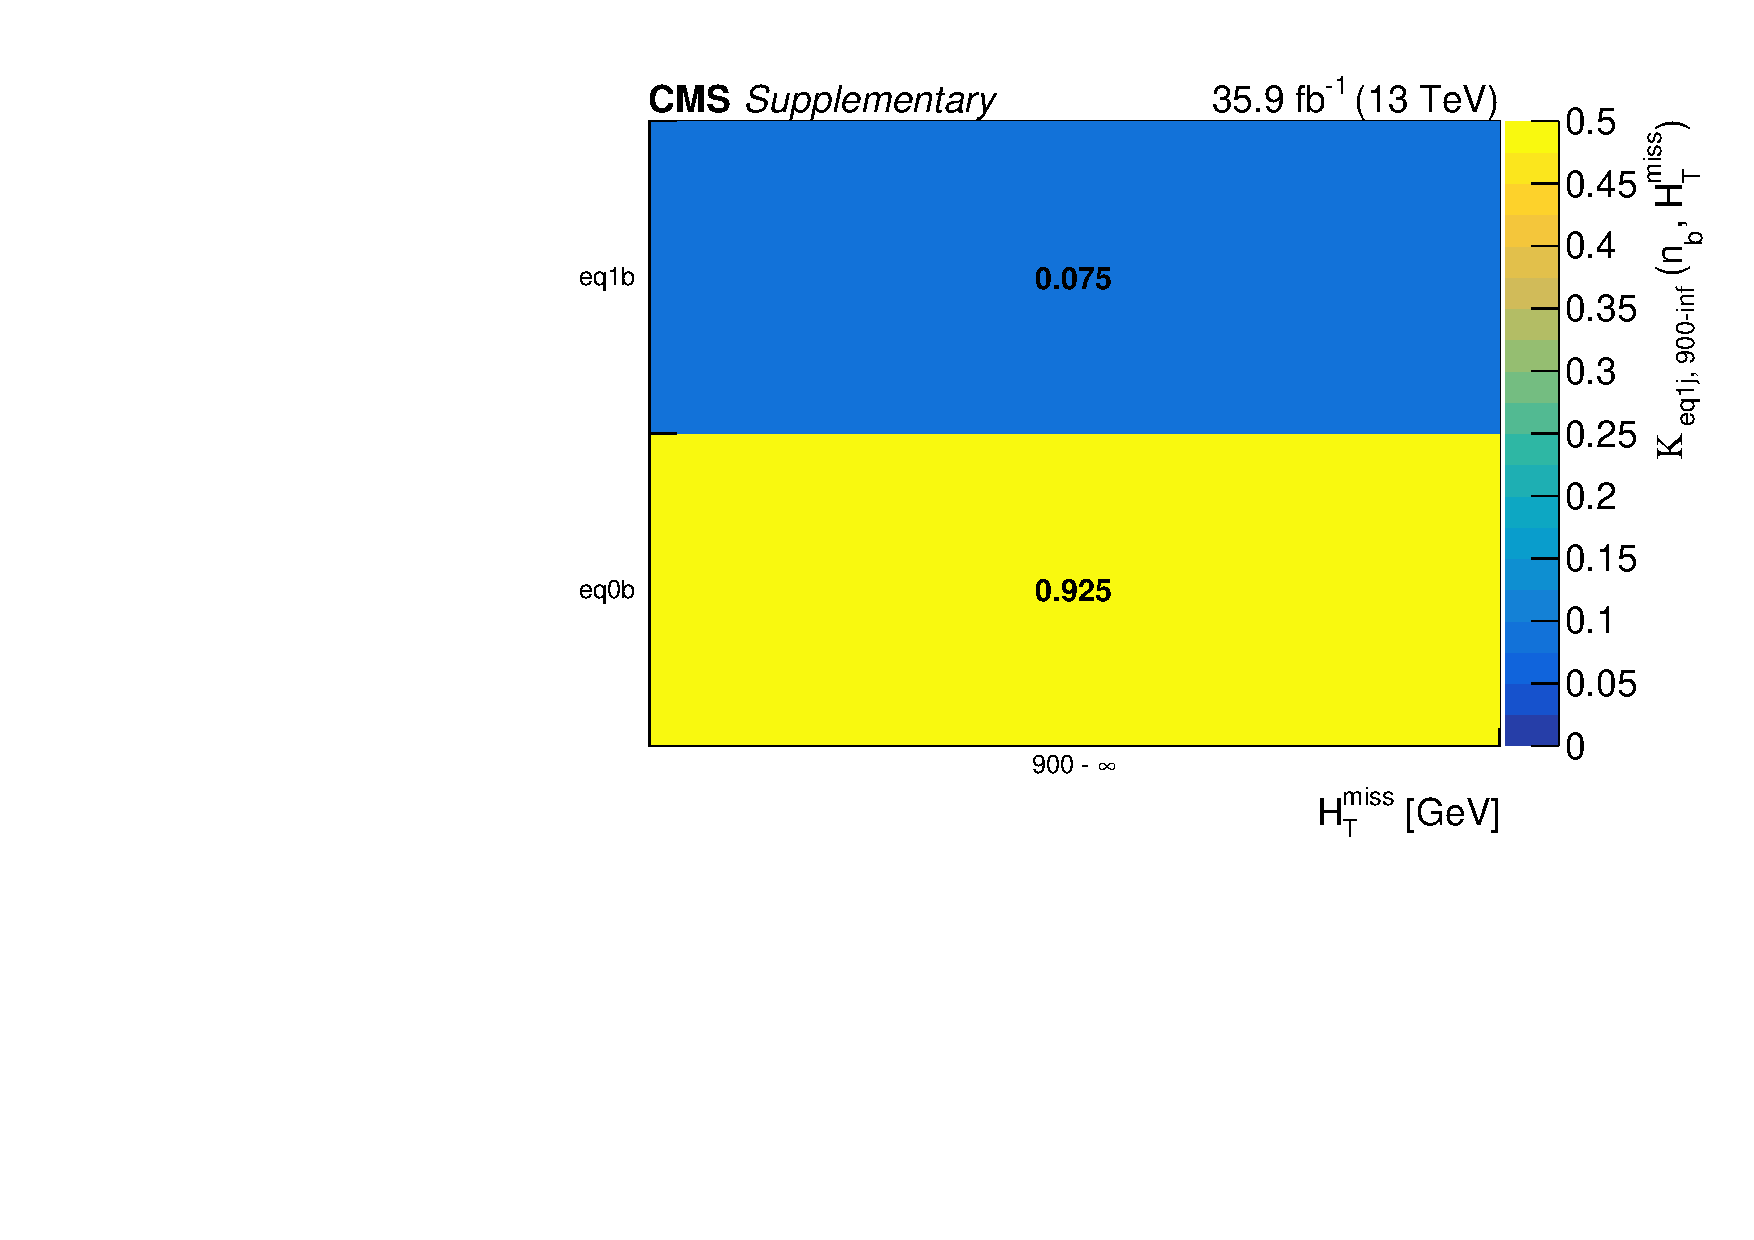
\includegraphics[width=0.3\textwidth]{figures/qcd/ewk_kappas/ewkKappa_eq1j_900-inf}
    } \\
    \caption{
        Electroweak (\ttw) monojet kappa factors used to distribute
        the QCD multijet prediction across the \nb and \mht dimensions.
    }
    \label{fig:ewk_kappas_eq1j}
\end{figure}

\begin{figure}[!h]
    \centering
    \subfigure[$200<\scalht<250$ \gev]{
        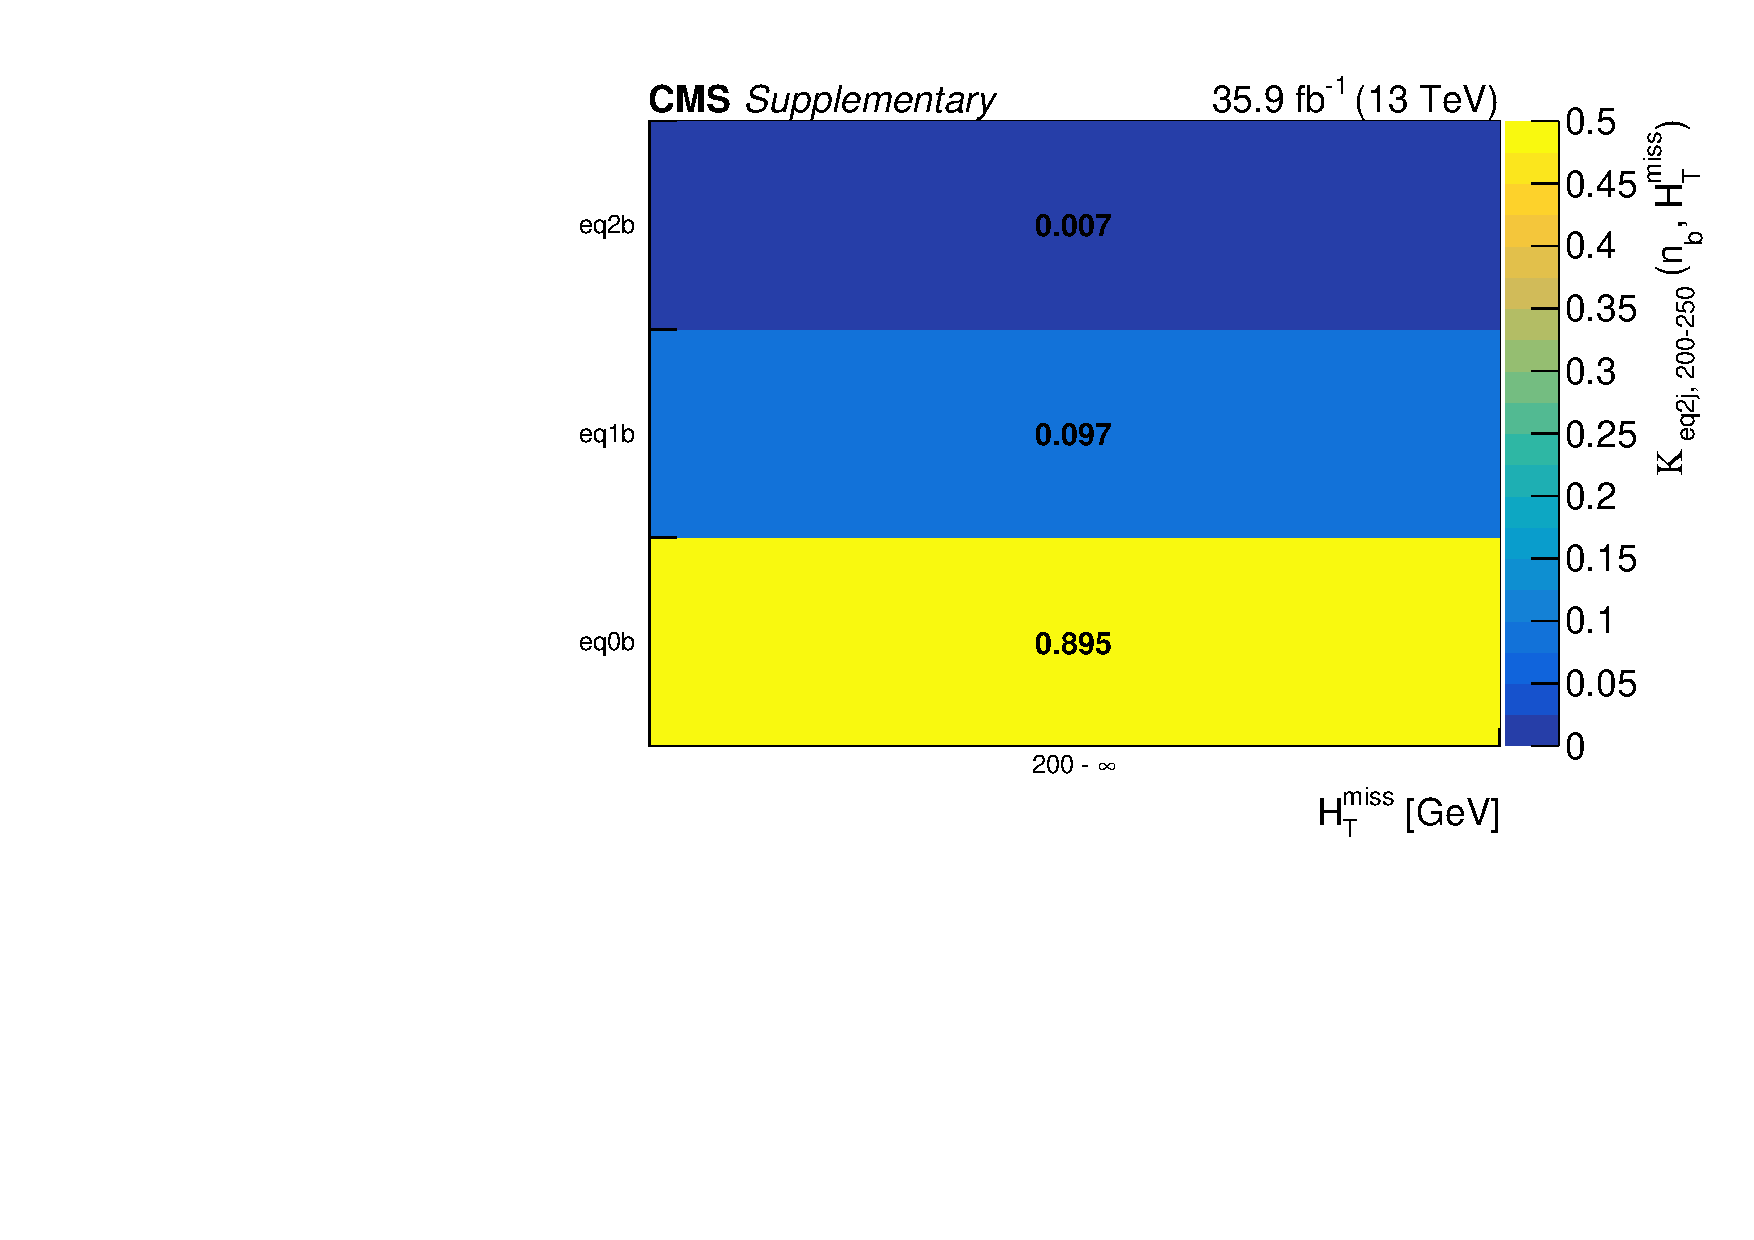
\includegraphics[width=0.3\textwidth]{figures/qcd/ewk_kappas/ewkKappa_eq2j_200-250}
    } ~~
    \subfigure[$250<\scalht<300$ \gev]{
        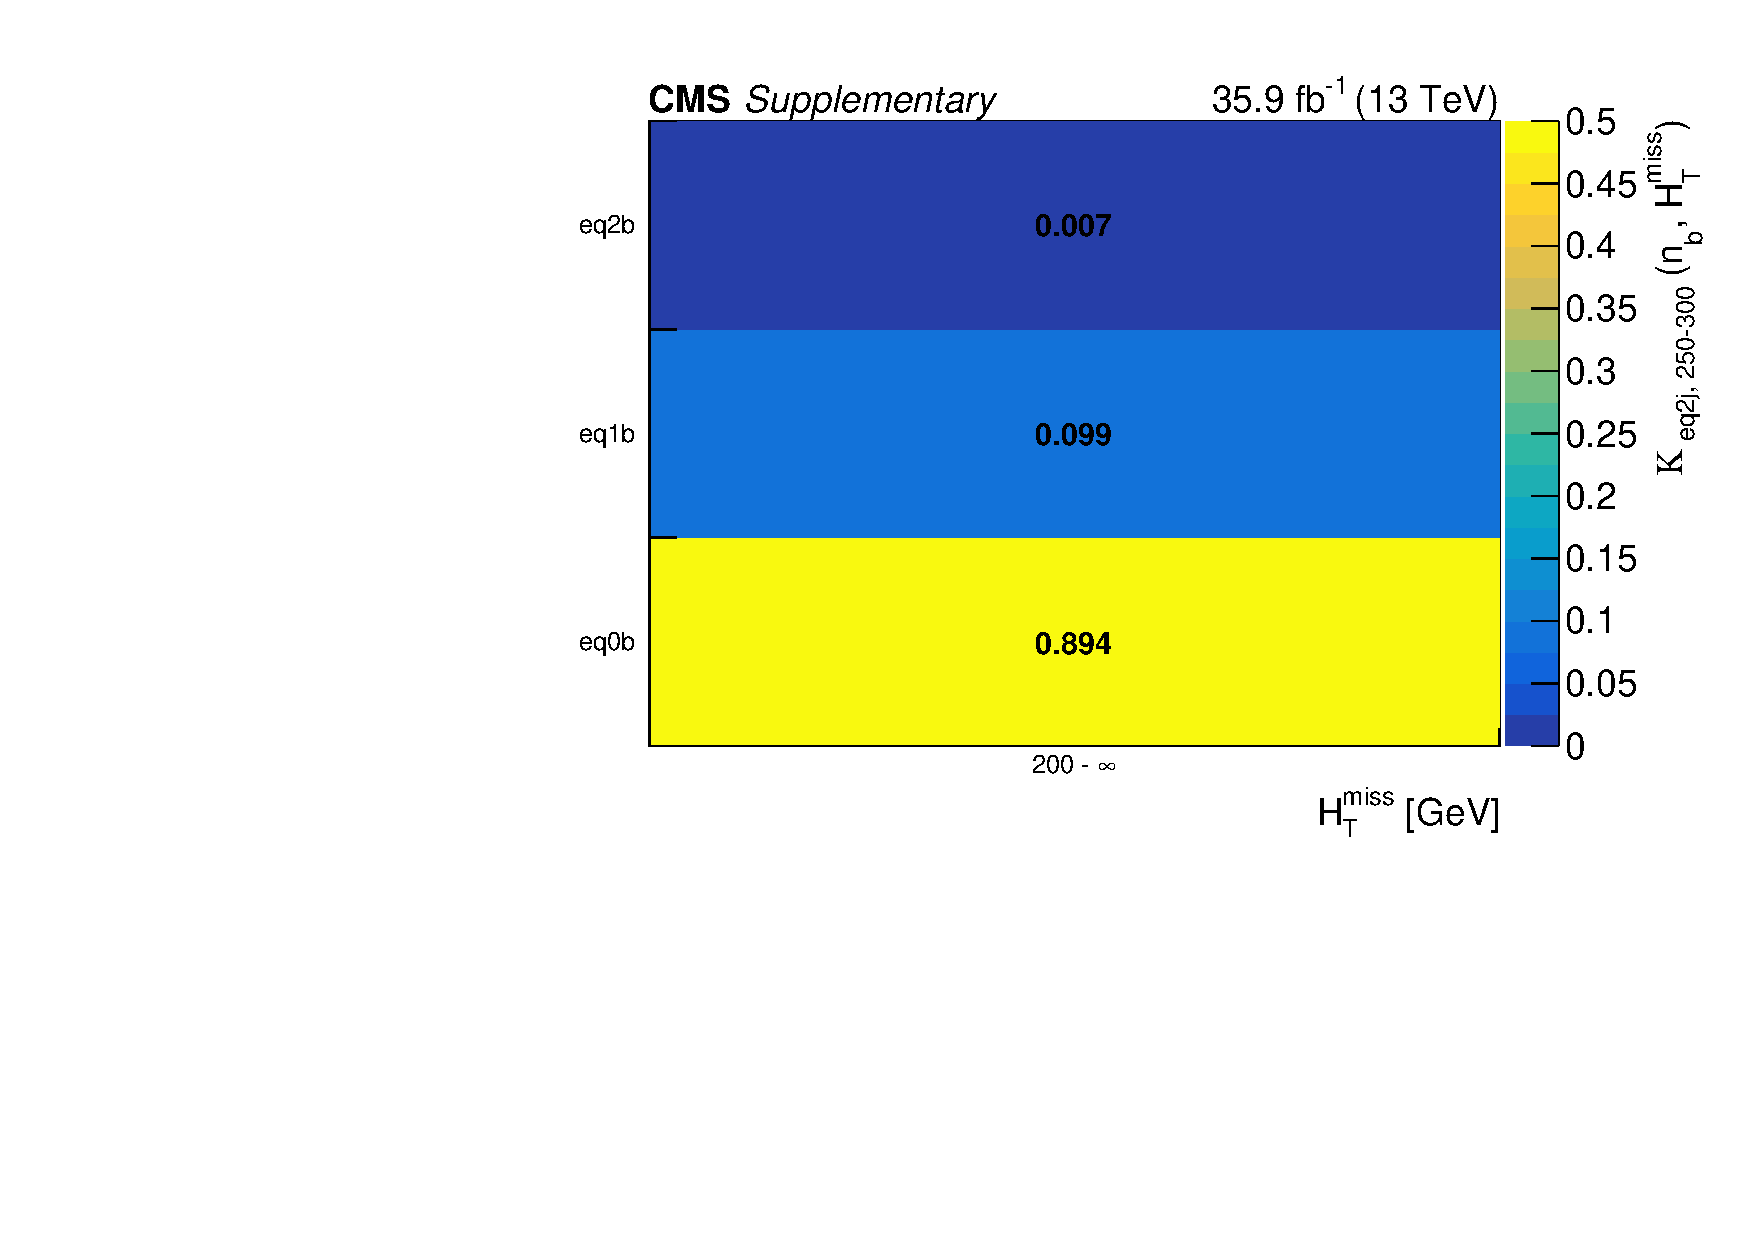
\includegraphics[width=0.3\textwidth]{figures/qcd/ewk_kappas/ewkKappa_eq2j_250-300}
    } ~~
    \subfigure[$300<\scalht<350$ \gev]{
        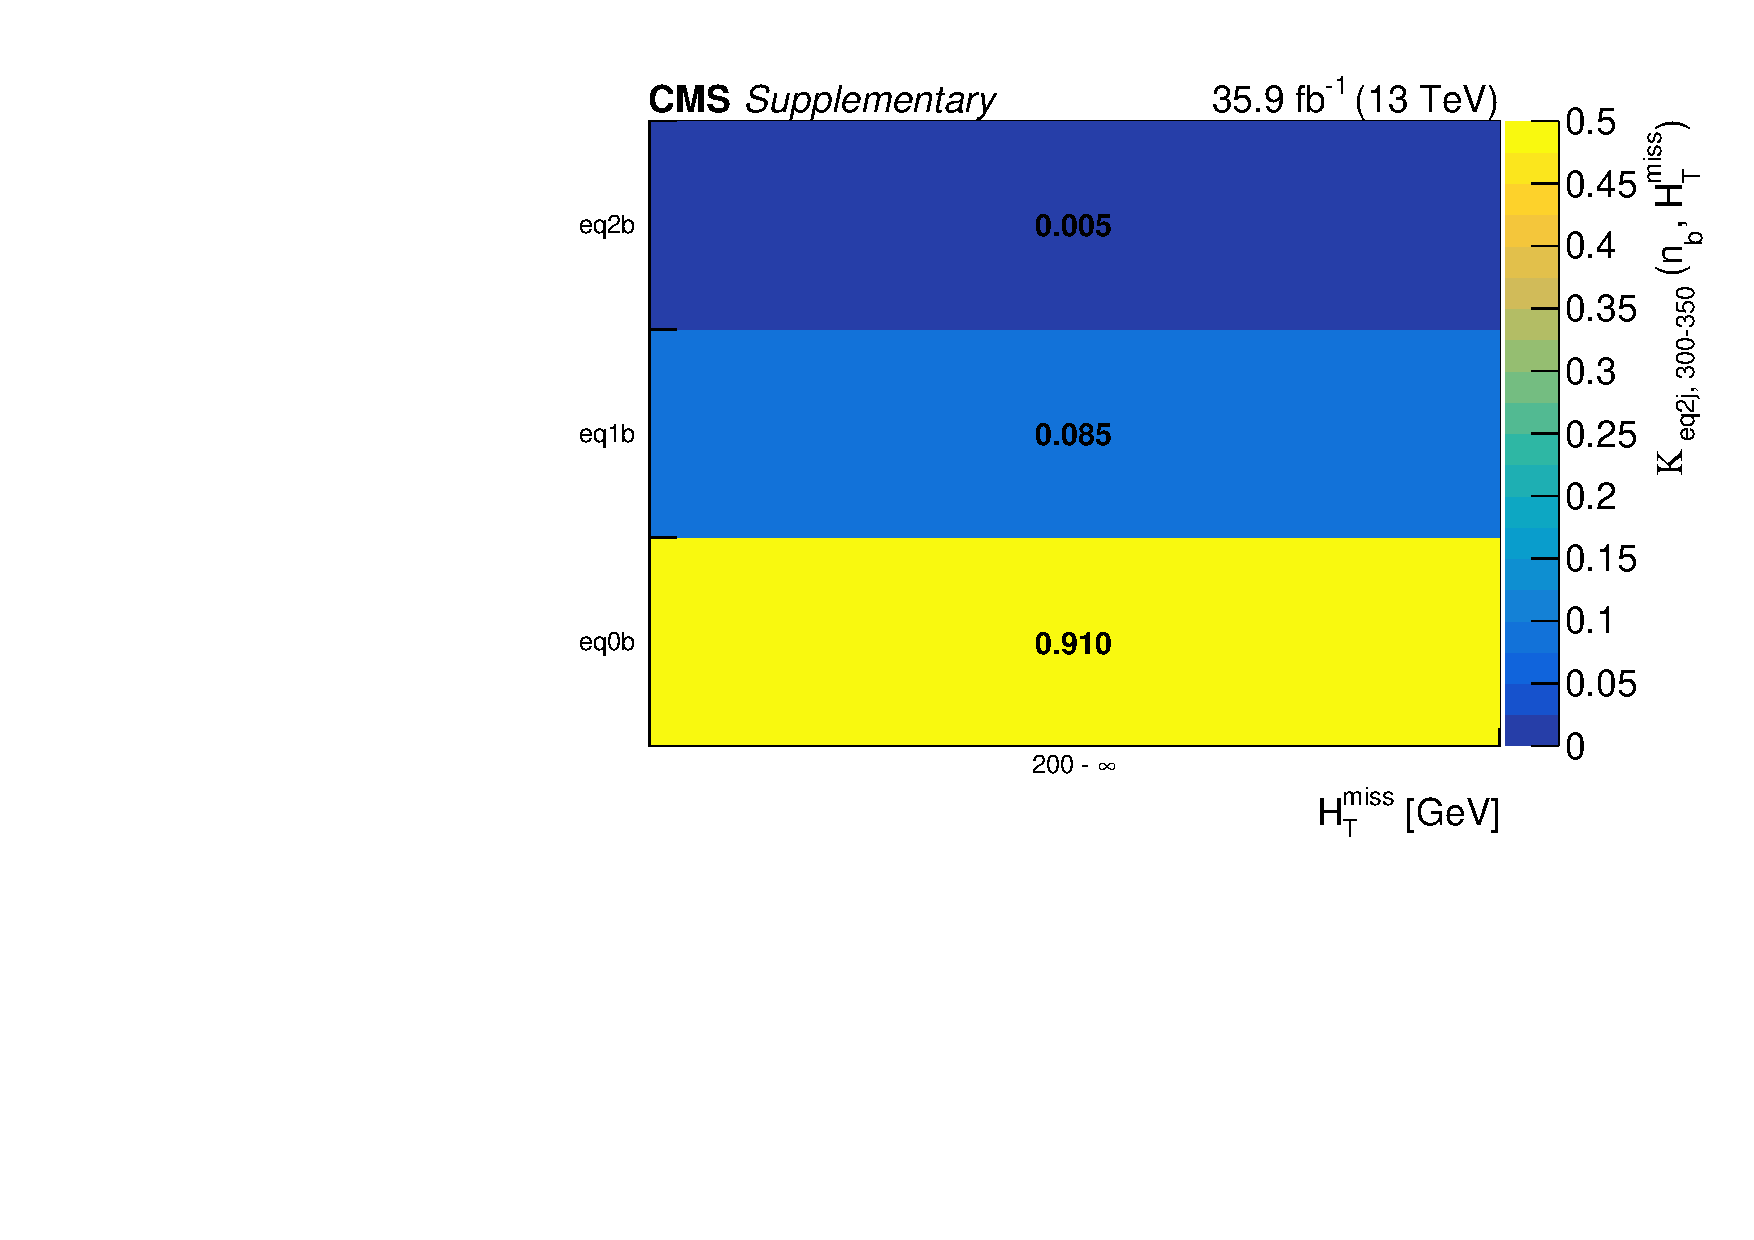
\includegraphics[width=0.3\textwidth]{figures/qcd/ewk_kappas/ewkKappa_eq2j_300-350}
    } \\
    \subfigure[$350<\scalht<400$ \gev]{
        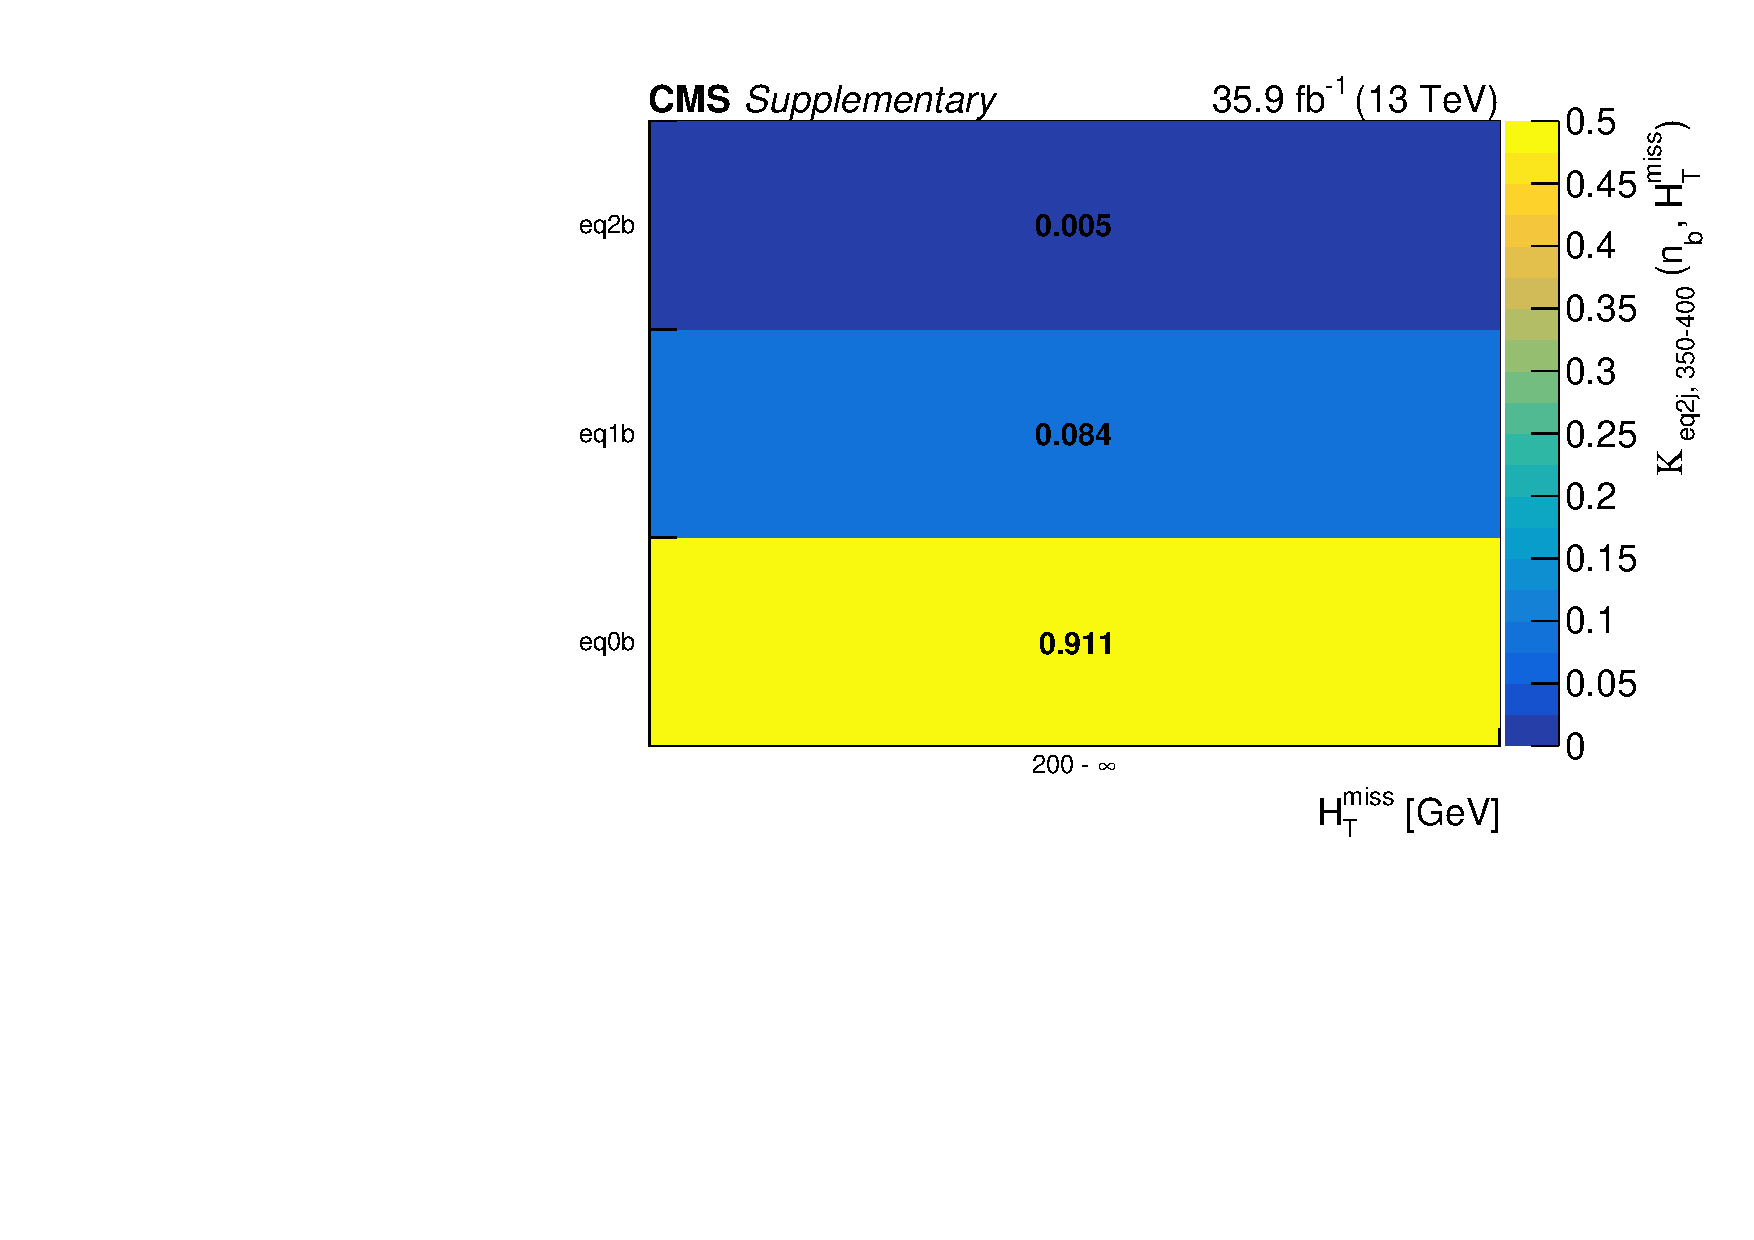
\includegraphics[width=0.3\textwidth]{figures/qcd/ewk_kappas/ewkKappa_eq2j_350-400}
    } ~~
    \subfigure[$400<\scalht<500$ \gev]{
        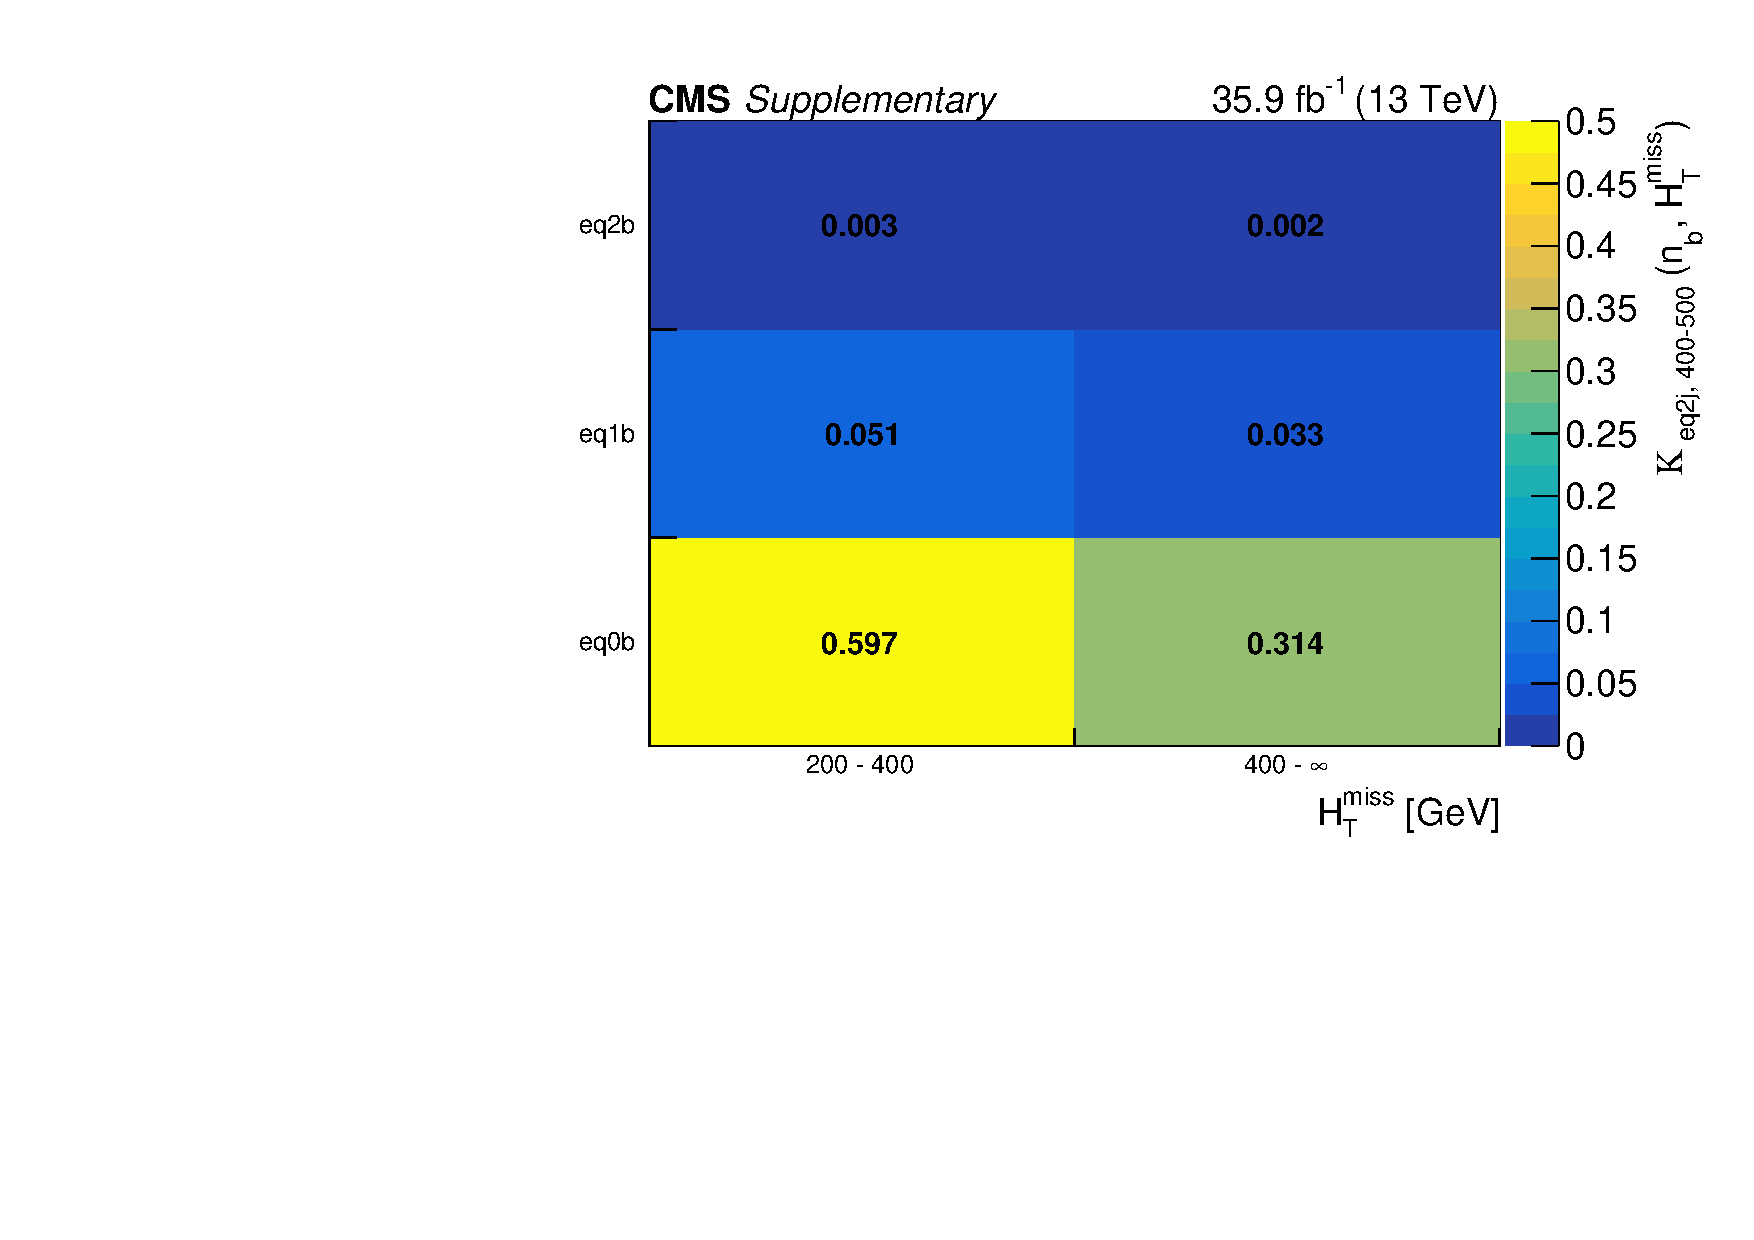
\includegraphics[width=0.3\textwidth]{figures/qcd/ewk_kappas/ewkKappa_eq2j_400-500}
    } ~~
    \subfigure[$500<\scalht<600$ \gev]{
        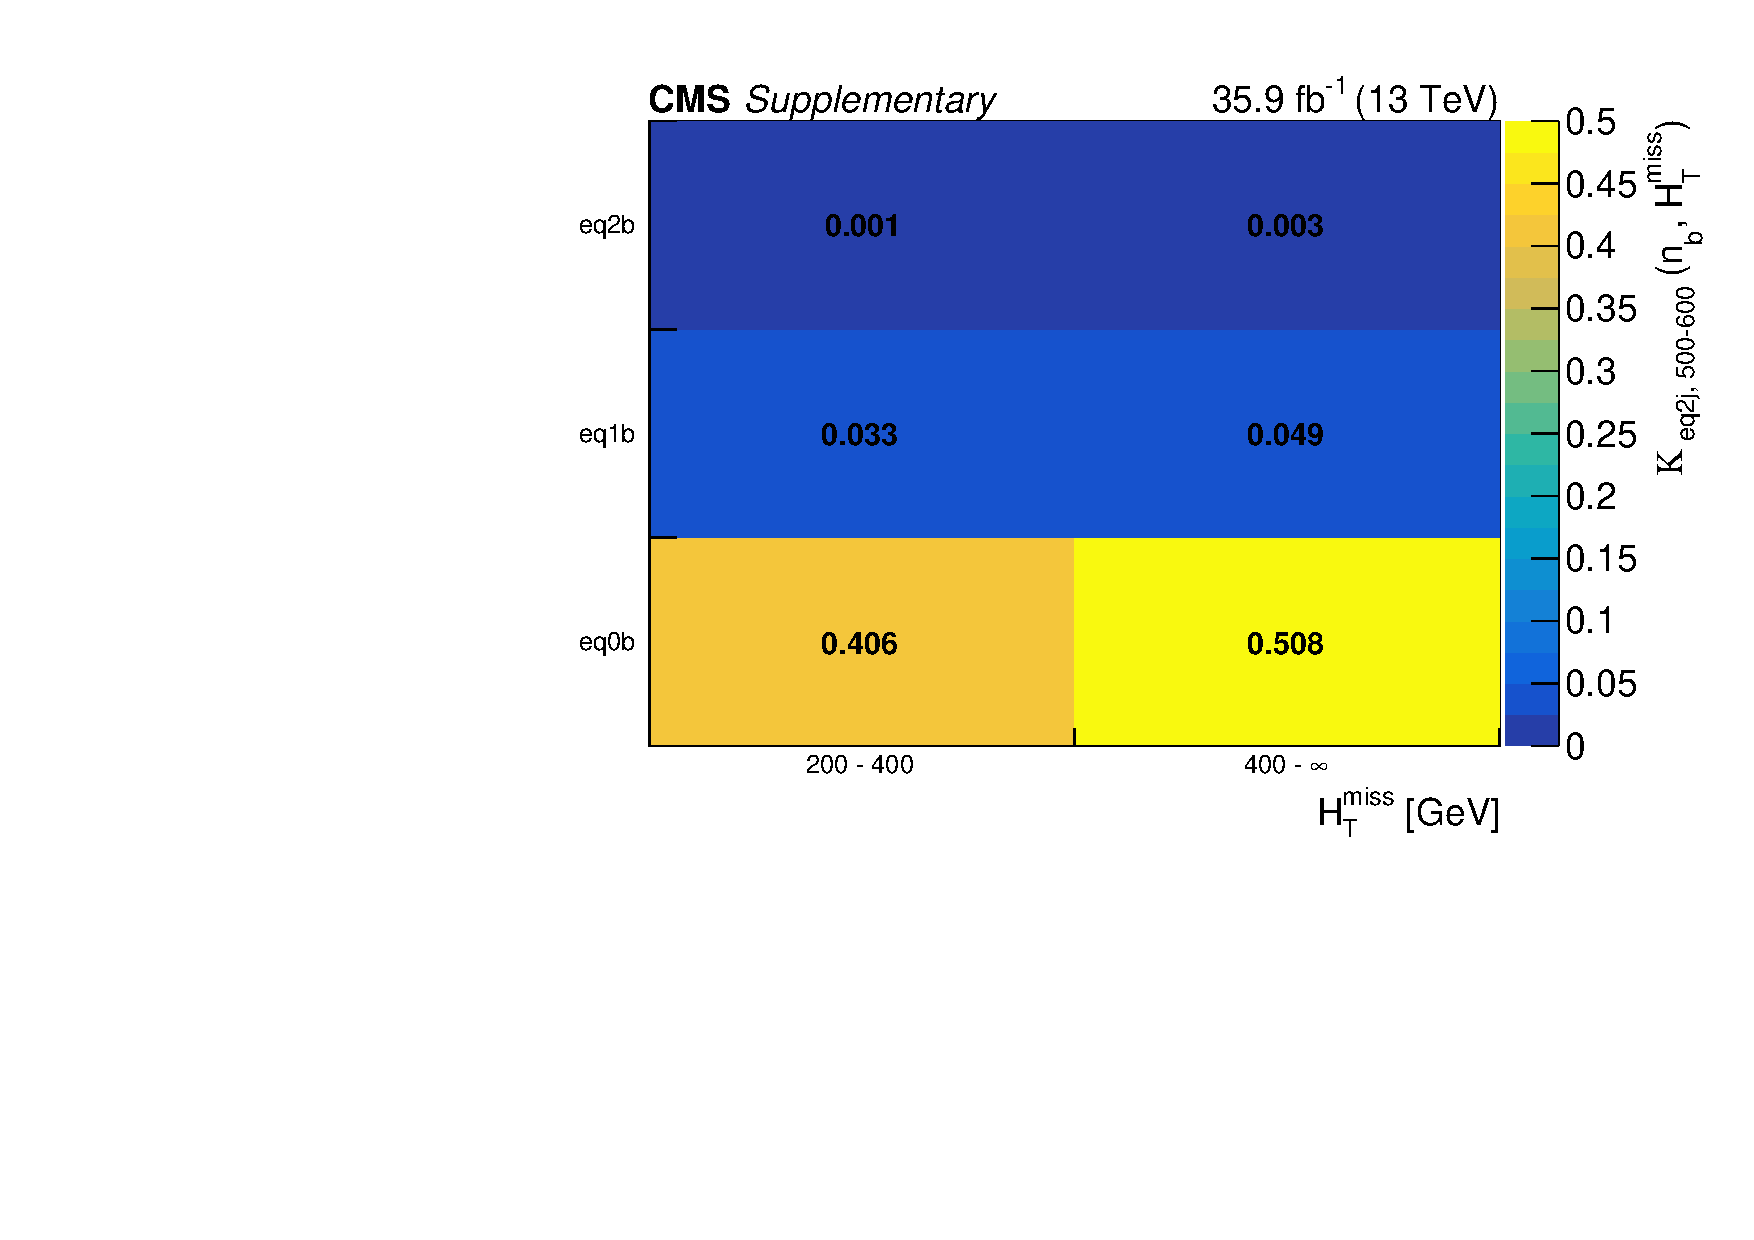
\includegraphics[width=0.3\textwidth]{figures/qcd/ewk_kappas/ewkKappa_eq2j_500-600}
    } \\
    \subfigure[$600<\scalht<750$ \gev]{
        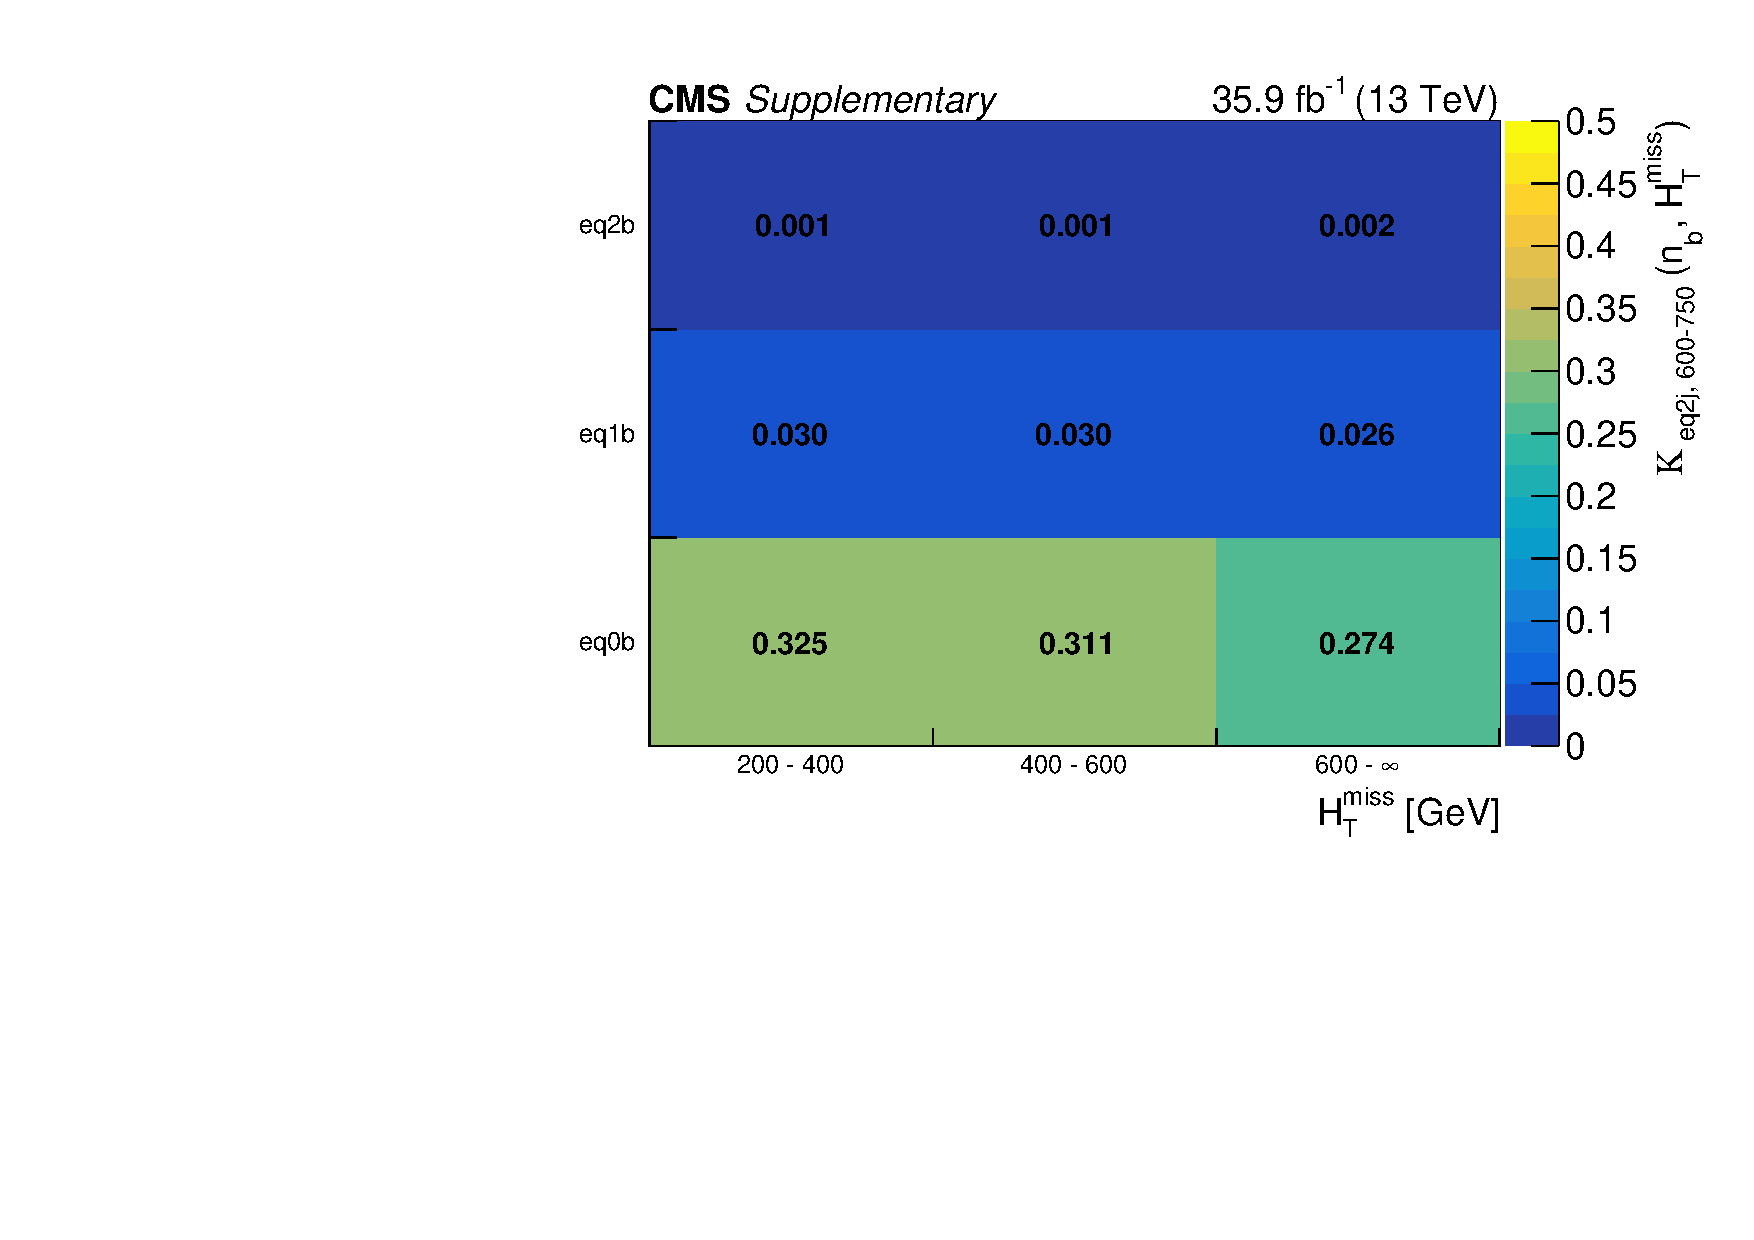
\includegraphics[width=0.3\textwidth]{figures/qcd/ewk_kappas/ewkKappa_eq2j_600-750}
    } ~~
    \subfigure[$750<\scalht<900$ \gev]{
        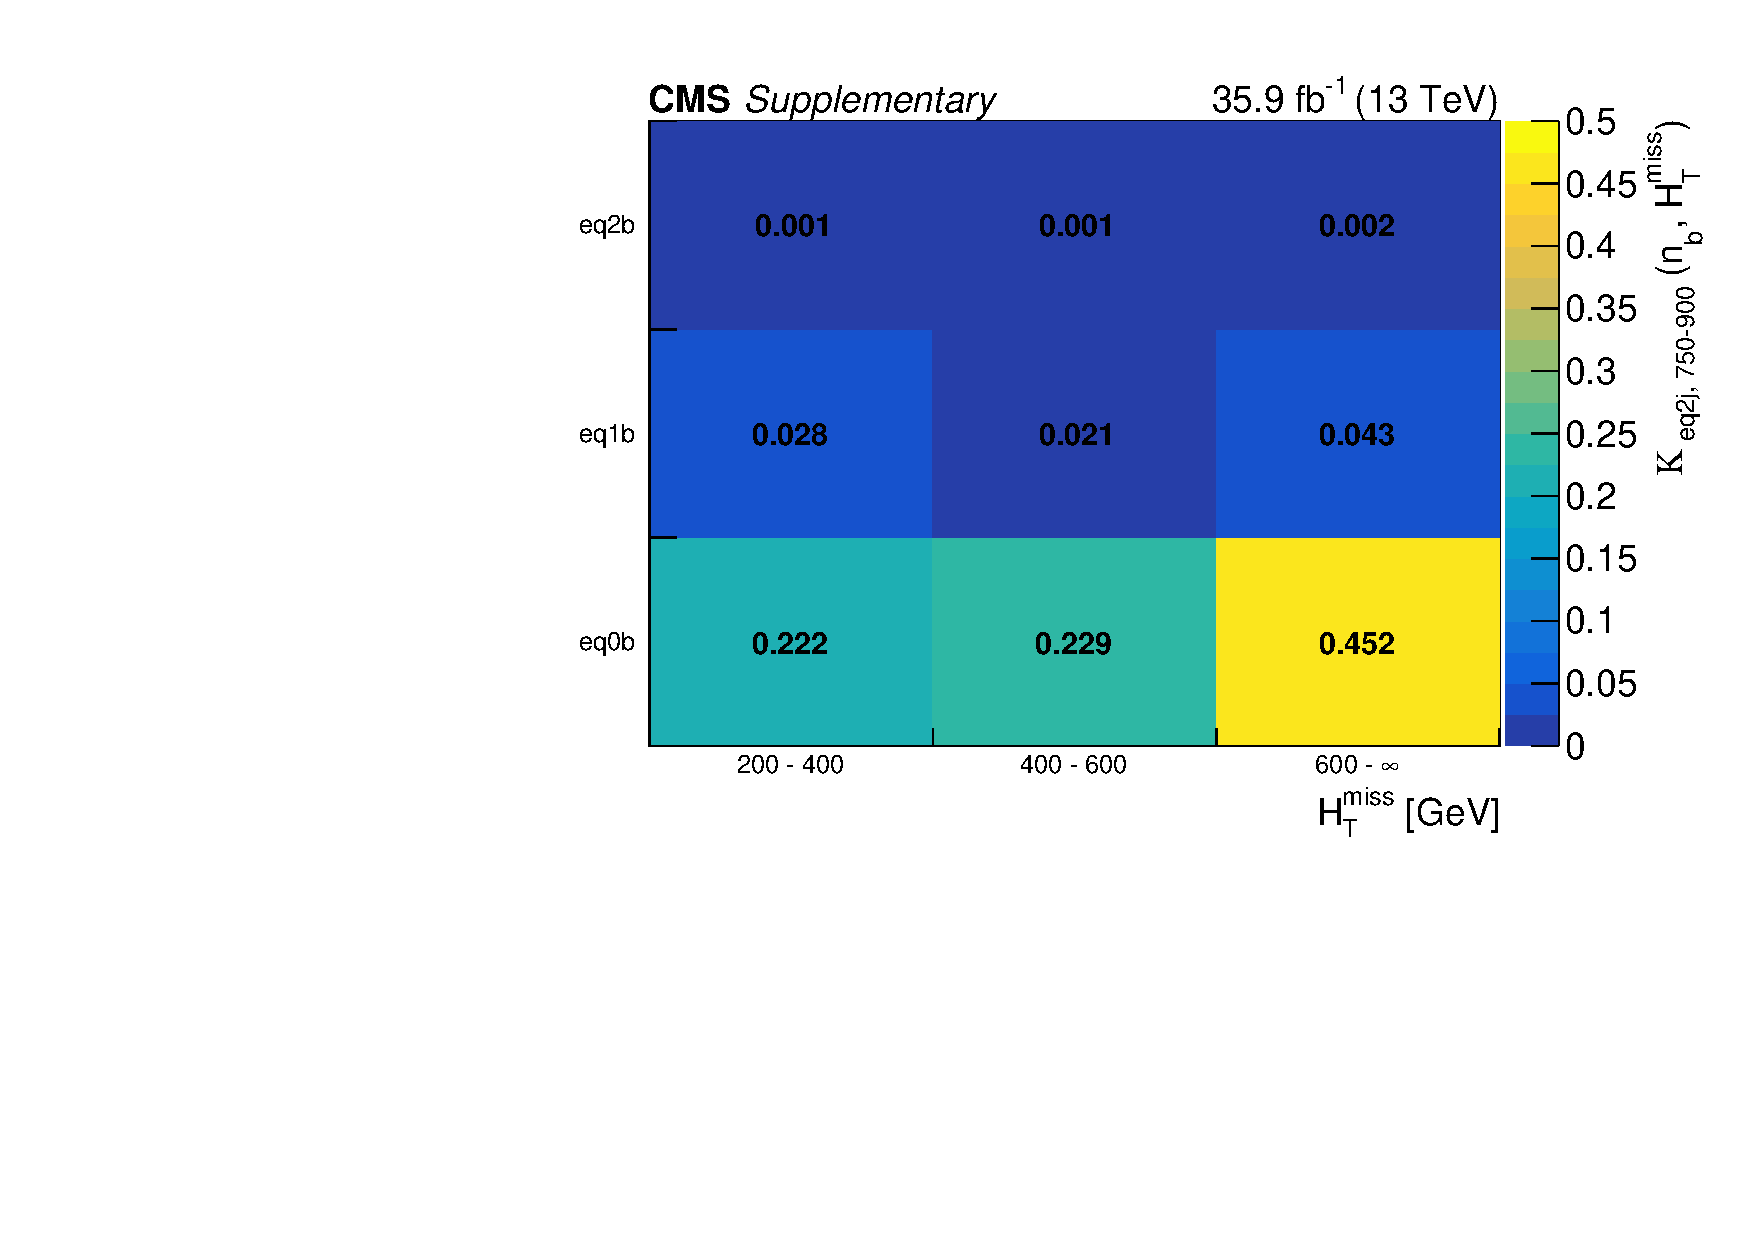
\includegraphics[width=0.3\textwidth]{figures/qcd/ewk_kappas/ewkKappa_eq2j_750-900}
    } ~~
    \subfigure[$900<\scalht<1050$ \gev]{
        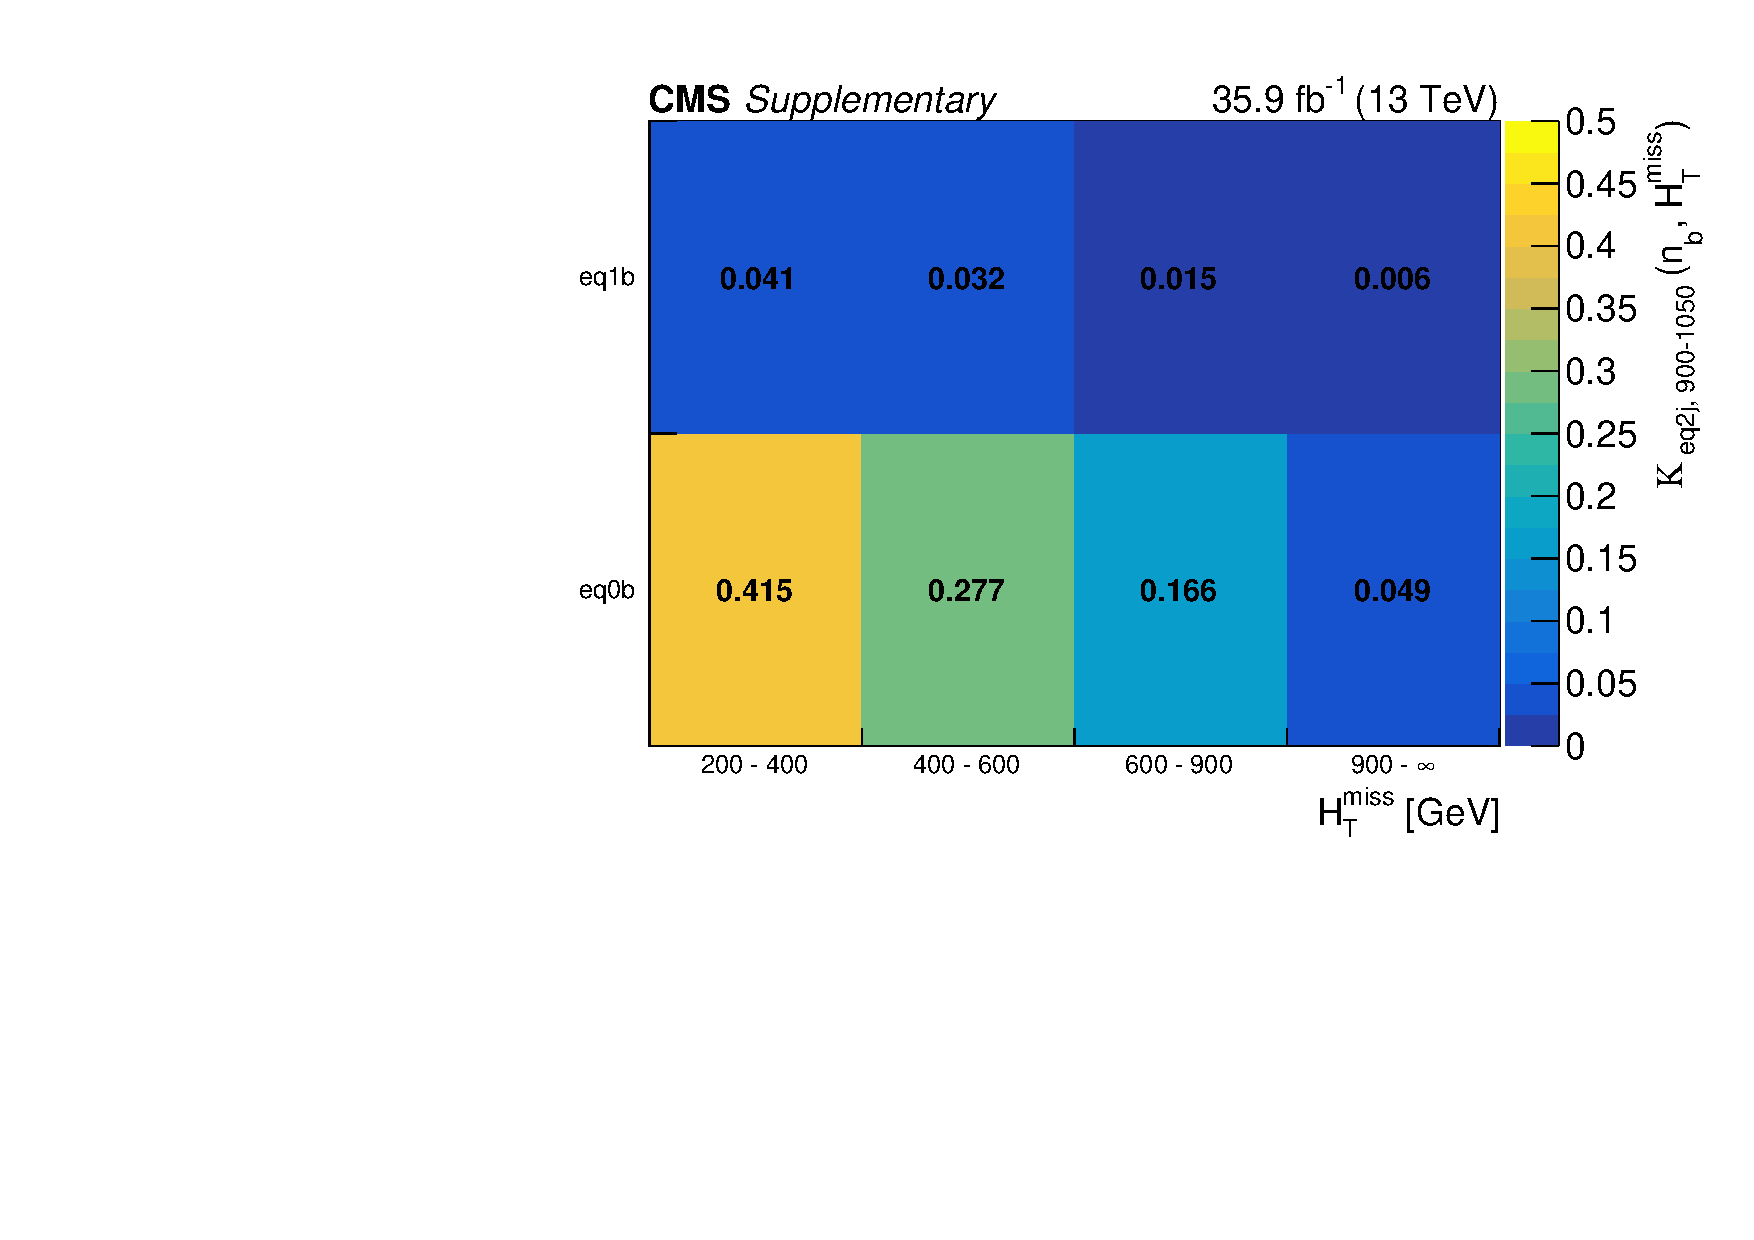
\includegraphics[width=0.3\textwidth]{figures/qcd/ewk_kappas/ewkKappa_eq2j_900-1050}
    } \\
    \subfigure[$1050<\scalht<1200$ \gev]{
        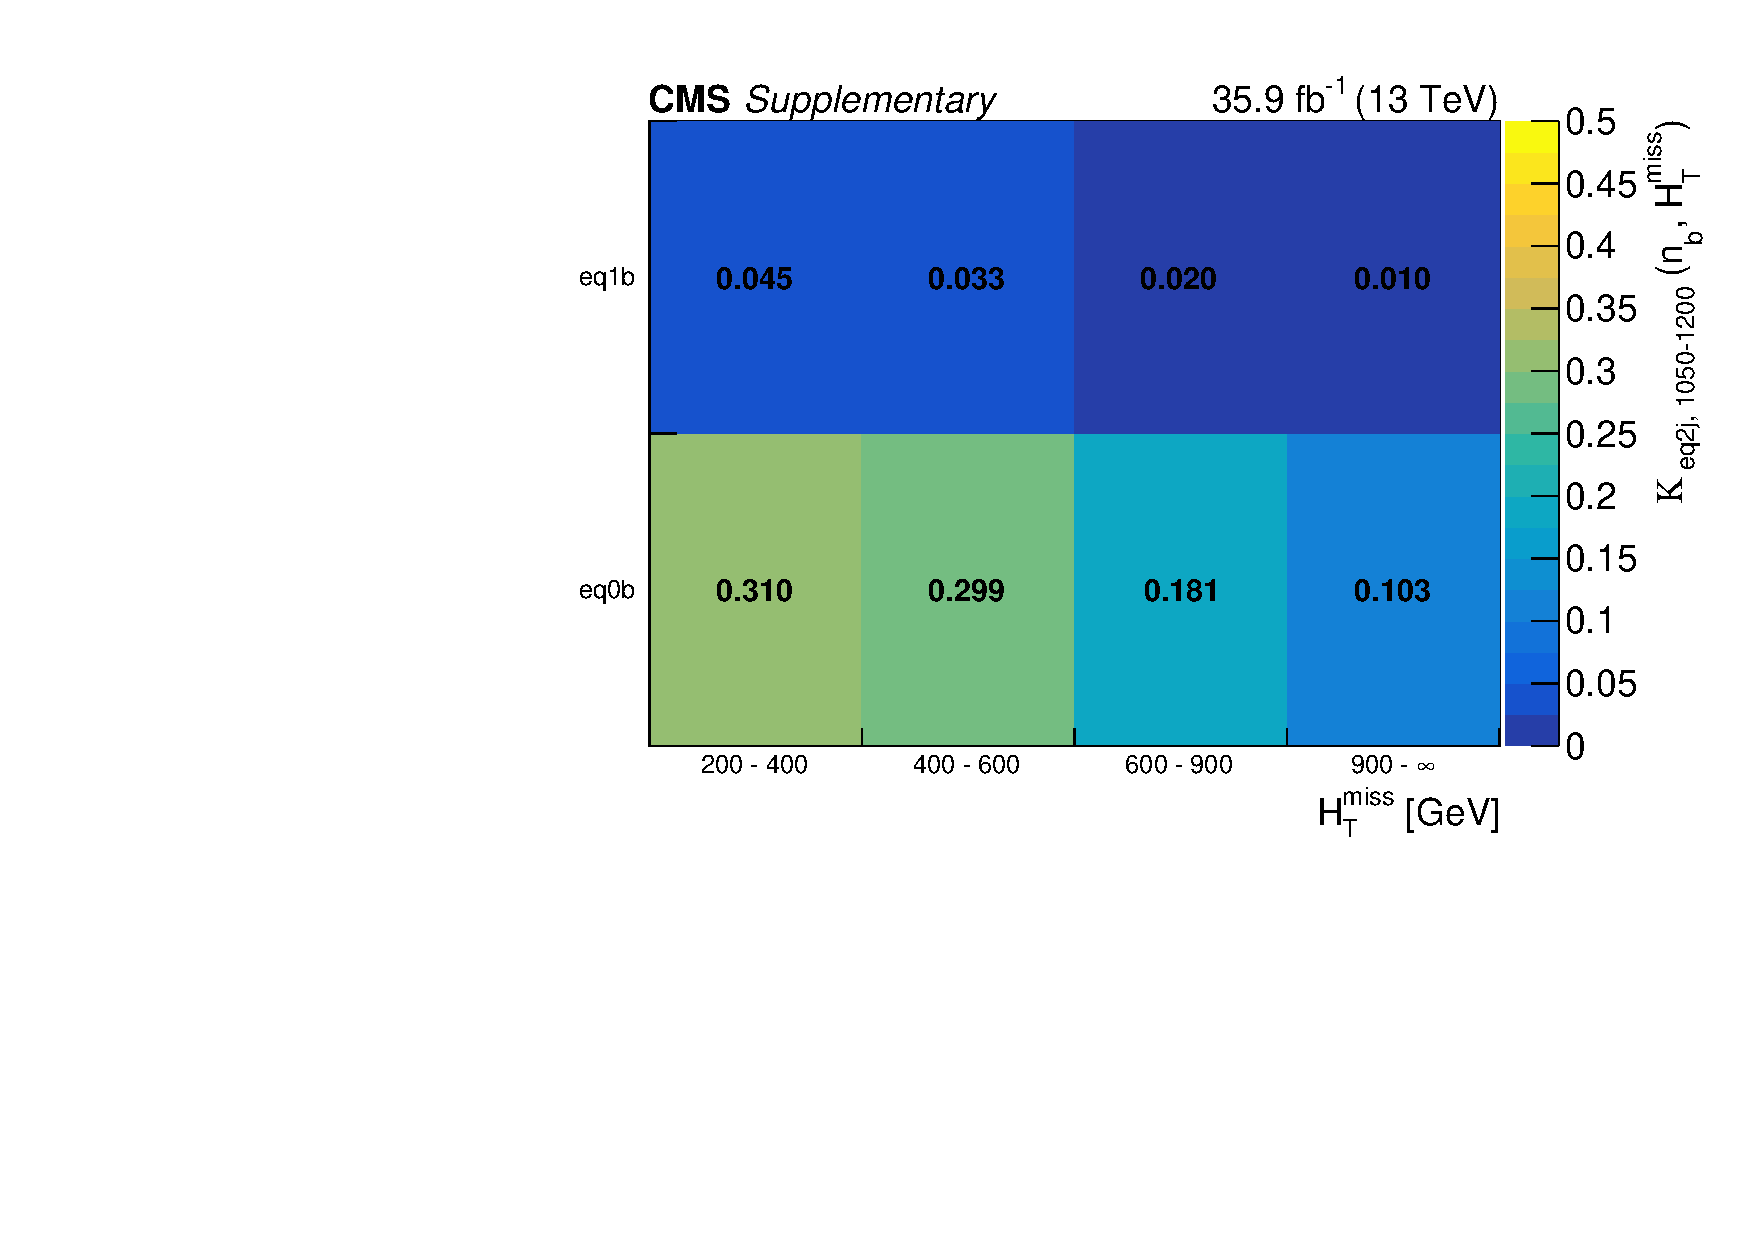
\includegraphics[width=0.3\textwidth]{figures/qcd/ewk_kappas/ewkKappa_eq2j_1050-1200}
    } ~~
    \subfigure[$900<\scalht<\infty$ \gev]{
        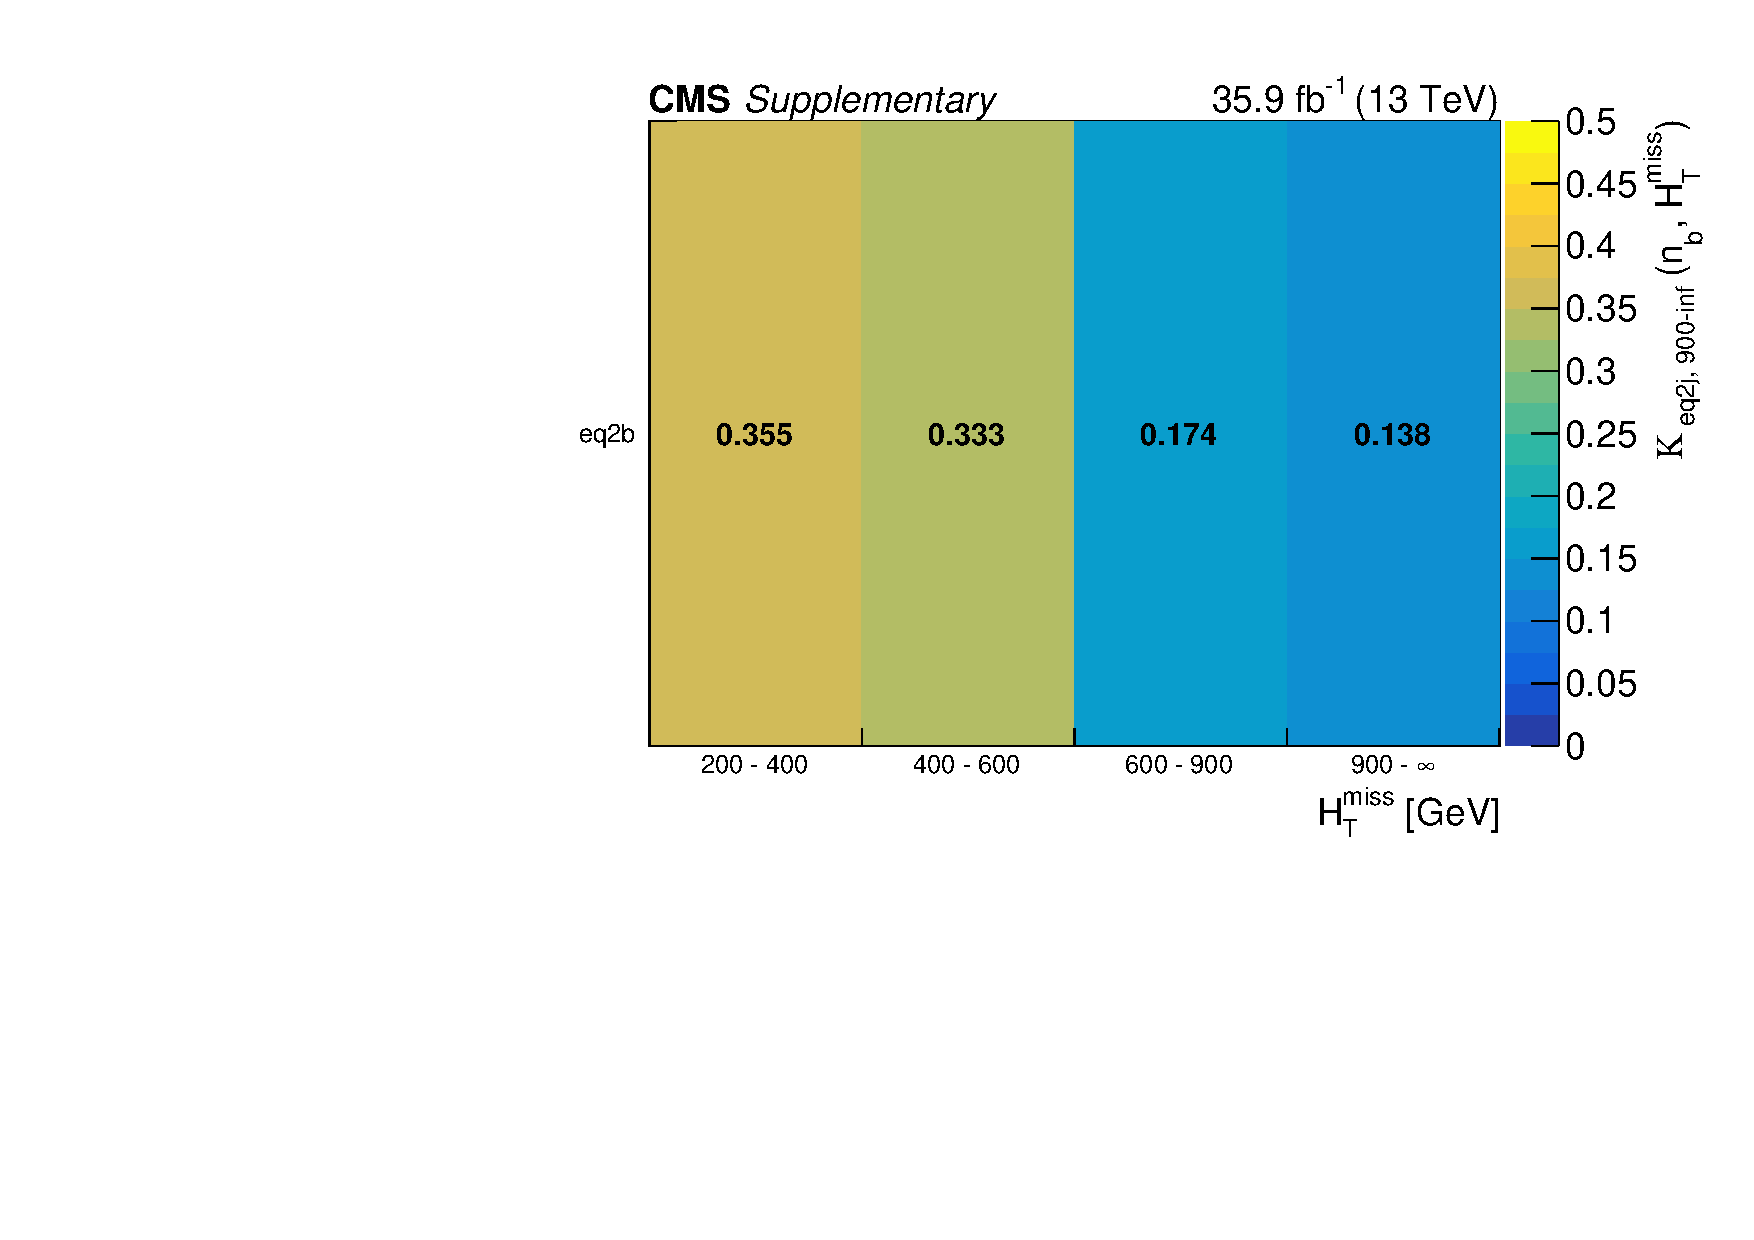
\includegraphics[width=0.3\textwidth]{figures/qcd/ewk_kappas/ewkKappa_eq2j_900-inf}
    } ~~
    \subfigure[$1200<\scalht<\infty$ \gev]{
        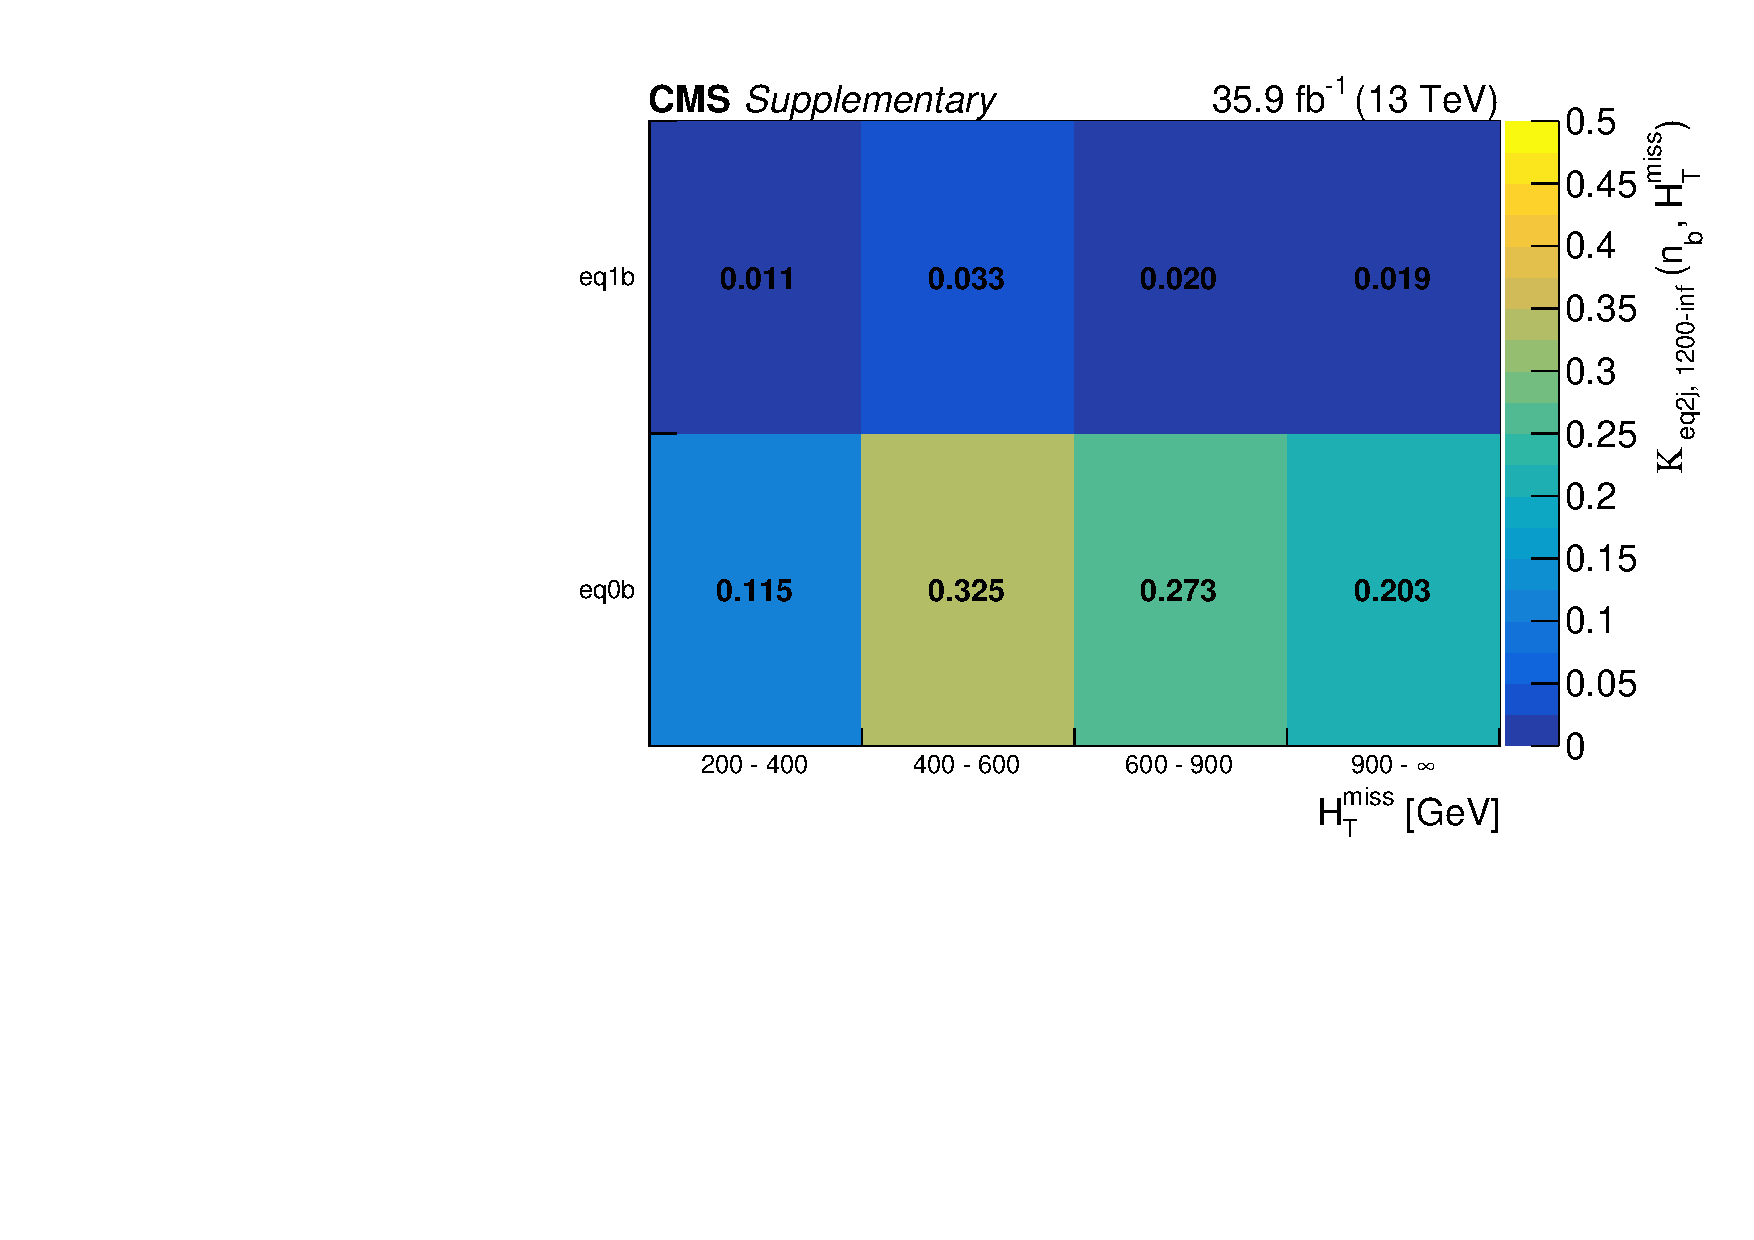
\includegraphics[width=0.3\textwidth]{figures/qcd/ewk_kappas/ewkKappa_eq2j_1200-inf}
    } \\
    \caption{
        Electroweak (\ttw) eq2j kappa factors used to distribute
        the QCD multijet prediction across the \nb and \mht dimensions.
    }
    \label{fig:ewk_kappas_eq2j}
\end{figure}

\begin{figure}[!h]
    \centering
    \subfigure[$200<\scalht<250$ \gev]{
        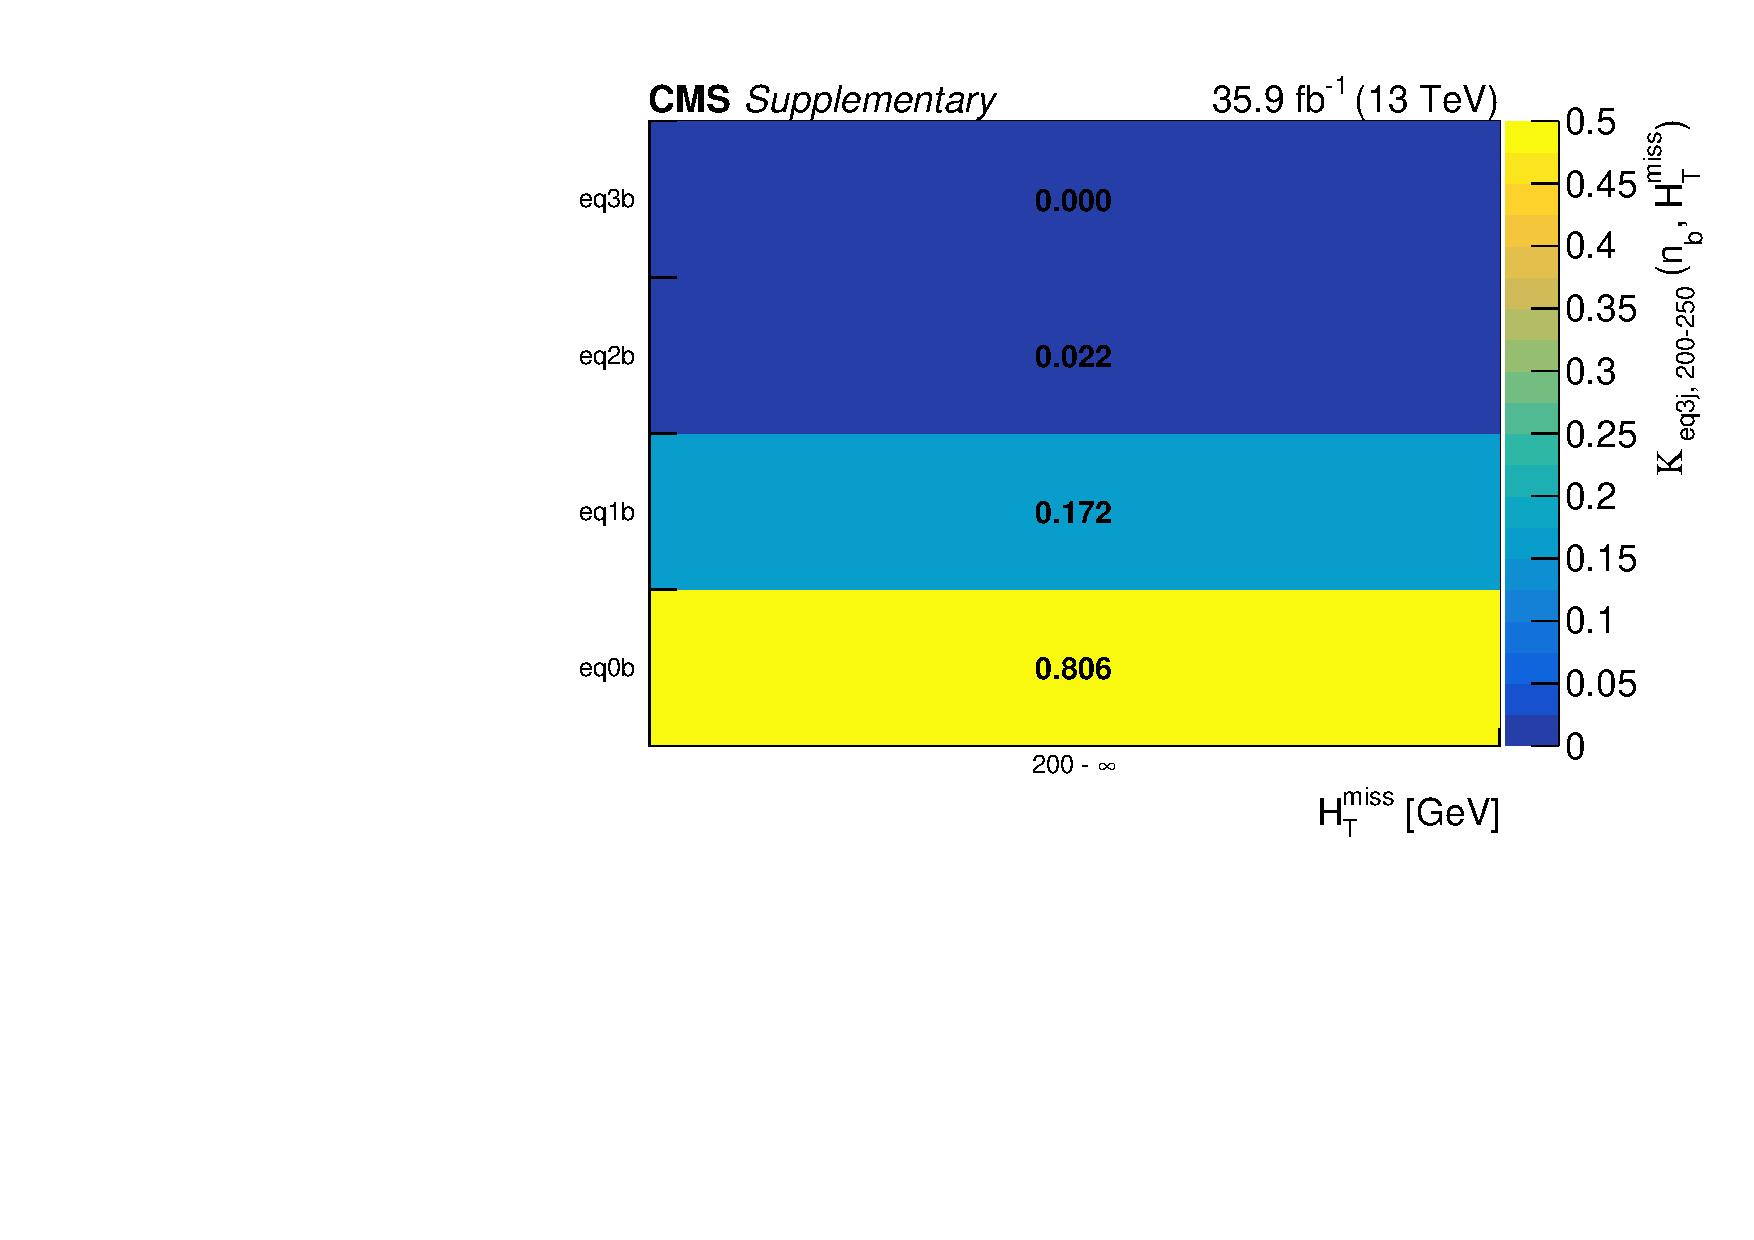
\includegraphics[width=0.3\textwidth]{figures/qcd/ewk_kappas/ewkKappa_eq3j_200-250}
    } ~~
    \subfigure[$250<\scalht<300$ \gev]{
        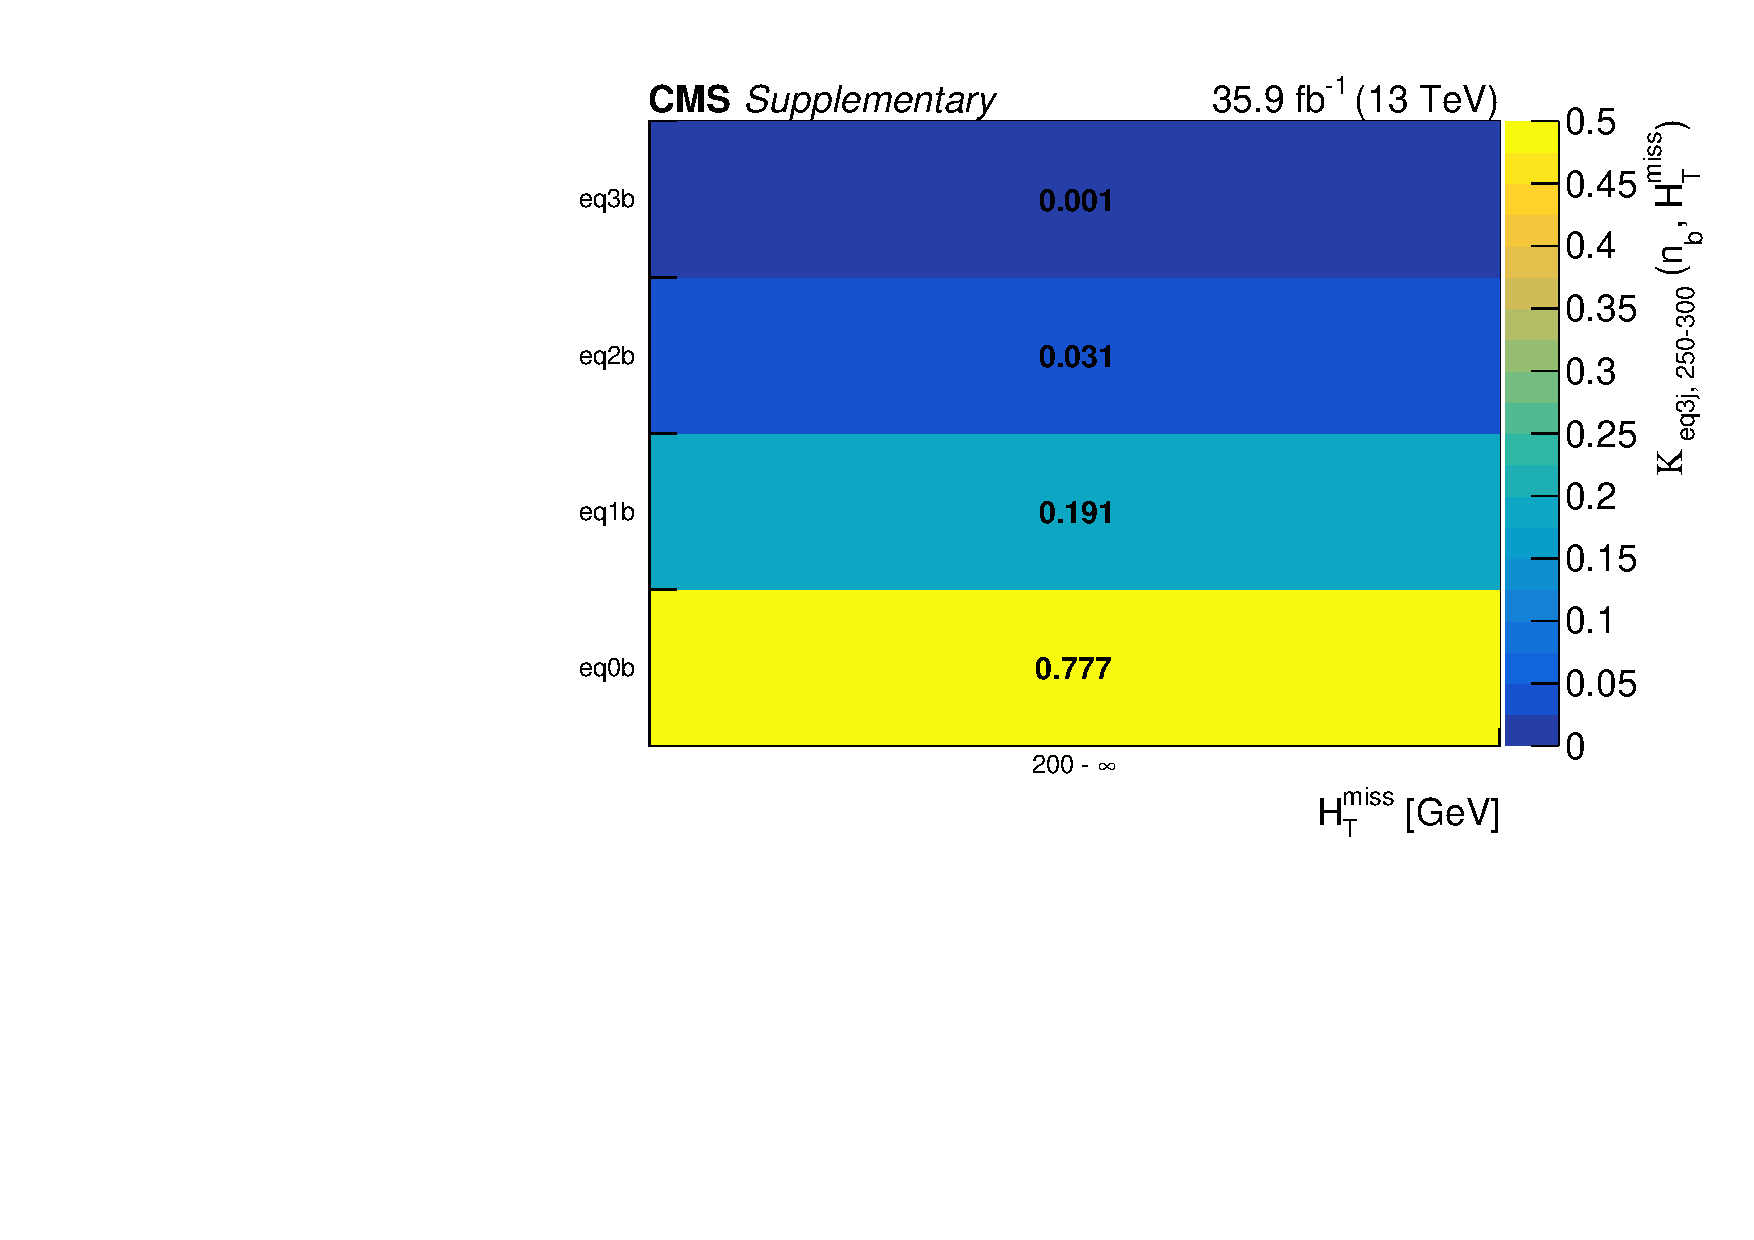
\includegraphics[width=0.3\textwidth]{figures/qcd/ewk_kappas/ewkKappa_eq3j_250-300}
    } ~~
    \subfigure[$300<\scalht<350$ \gev]{
        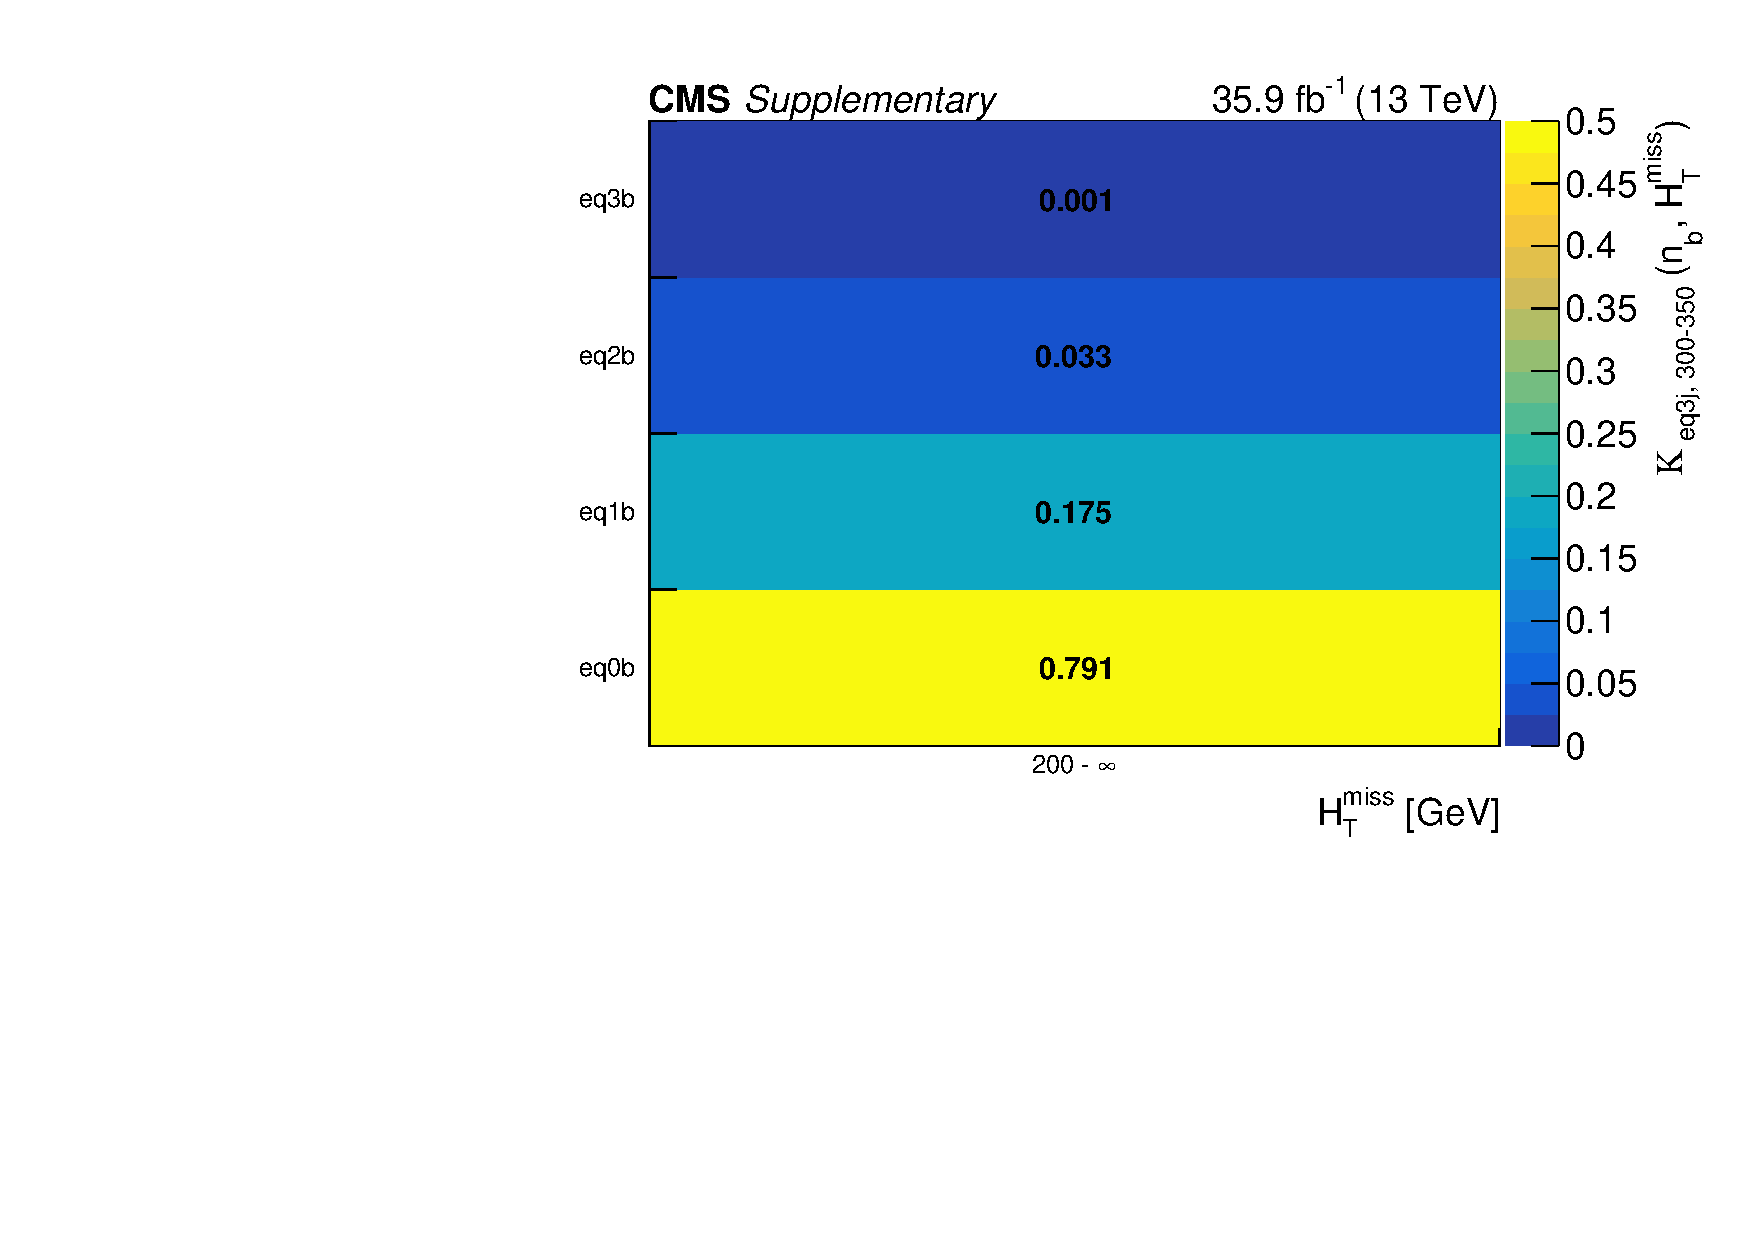
\includegraphics[width=0.3\textwidth]{figures/qcd/ewk_kappas/ewkKappa_eq3j_300-350}
    } \\
    \subfigure[$350<\scalht<400$ \gev]{
        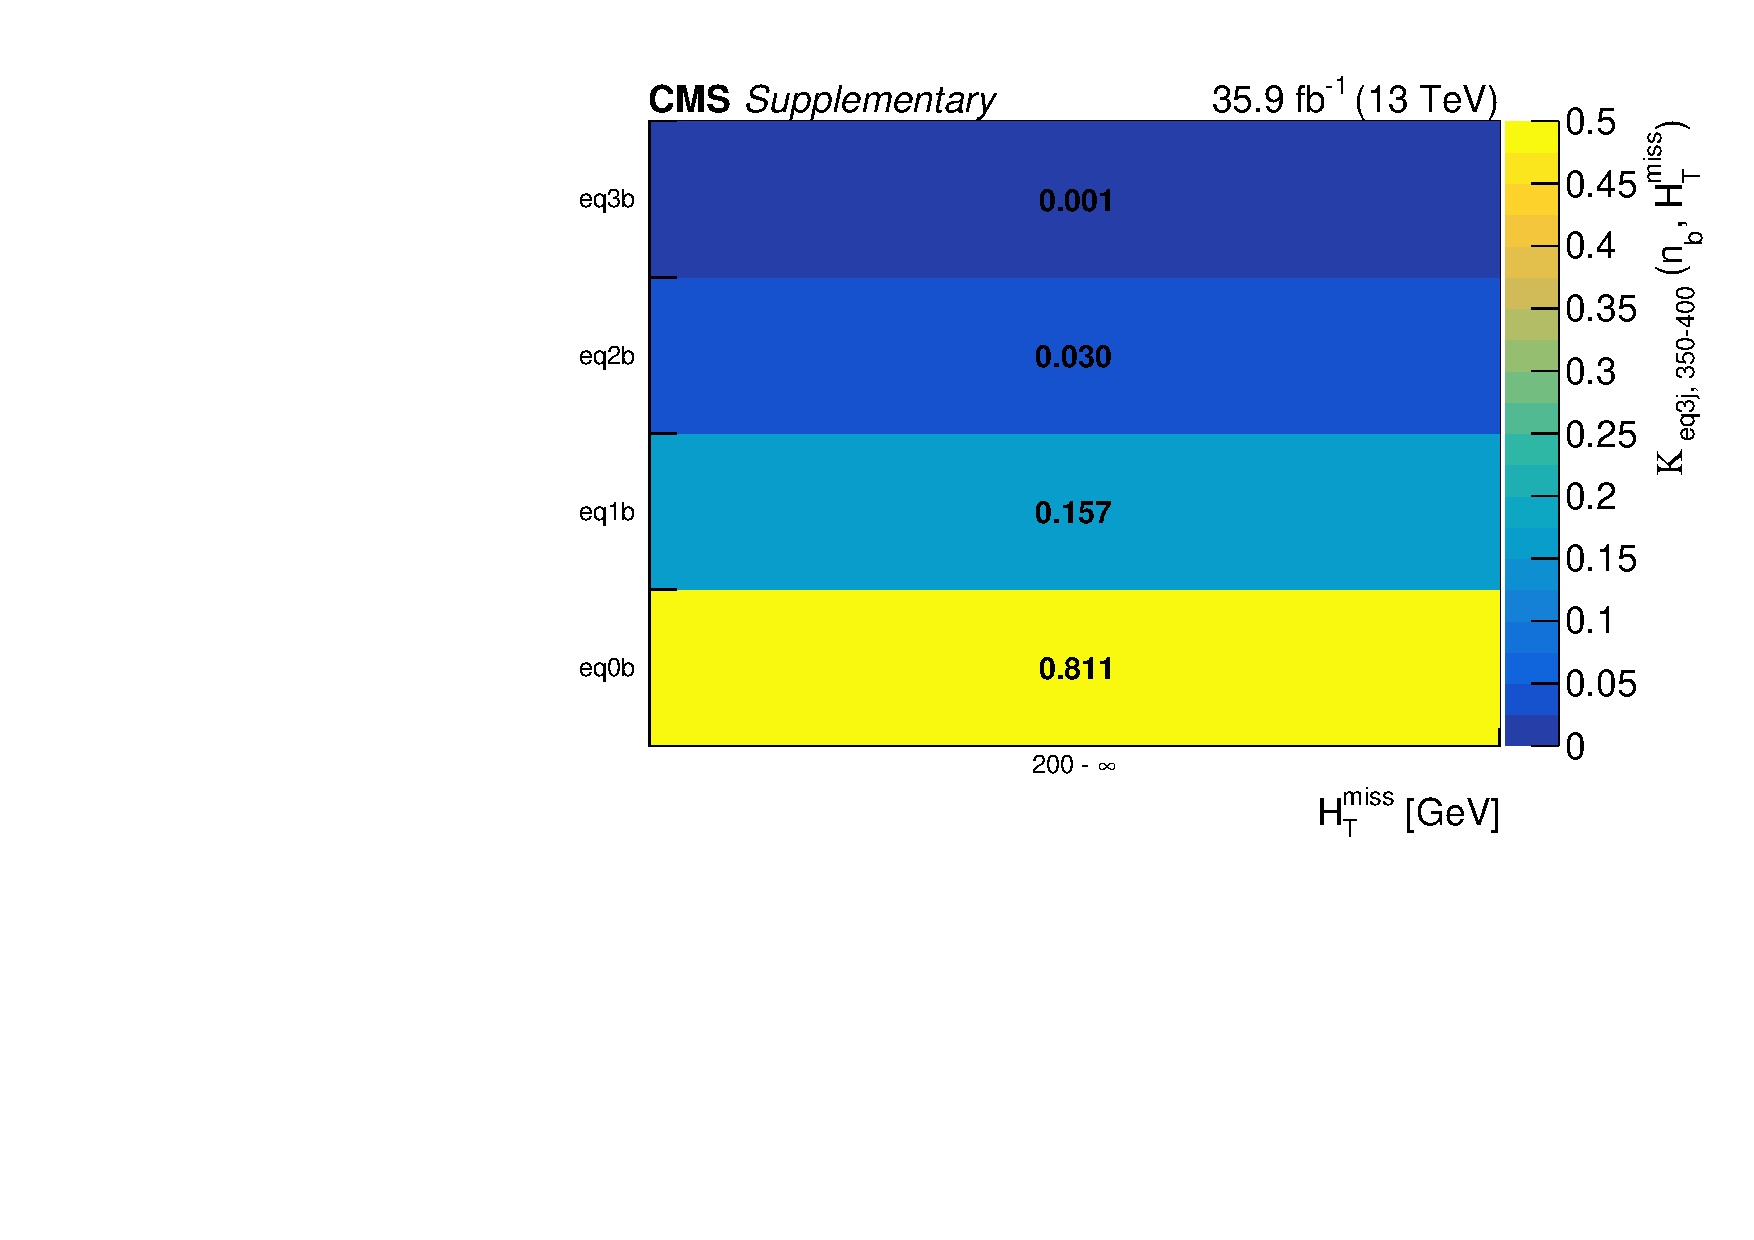
\includegraphics[width=0.3\textwidth]{figures/qcd/ewk_kappas/ewkKappa_eq3j_350-400}
    } ~~
    \subfigure[$400<\scalht<500$ \gev]{
        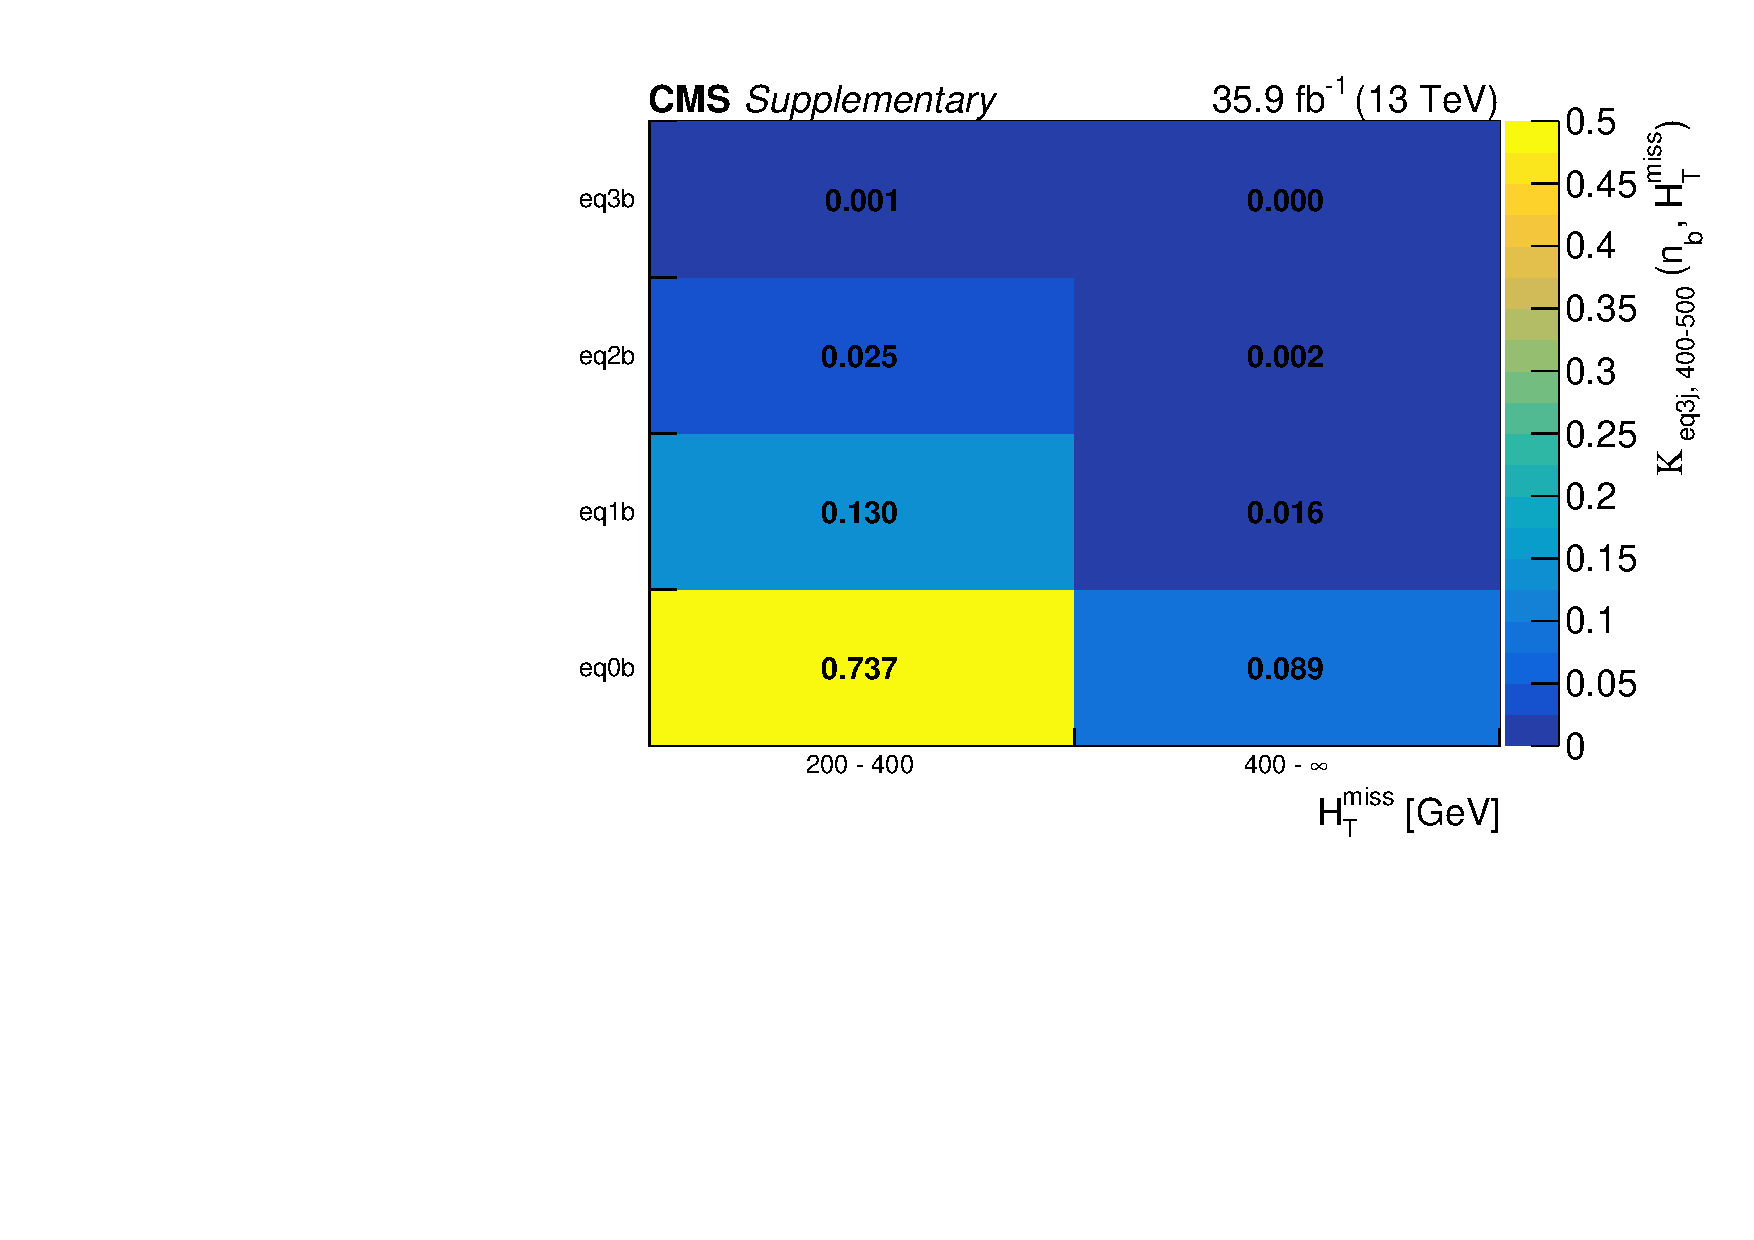
\includegraphics[width=0.3\textwidth]{figures/qcd/ewk_kappas/ewkKappa_eq3j_400-500}
    } ~~
    \subfigure[$500<\scalht<600$ \gev]{
        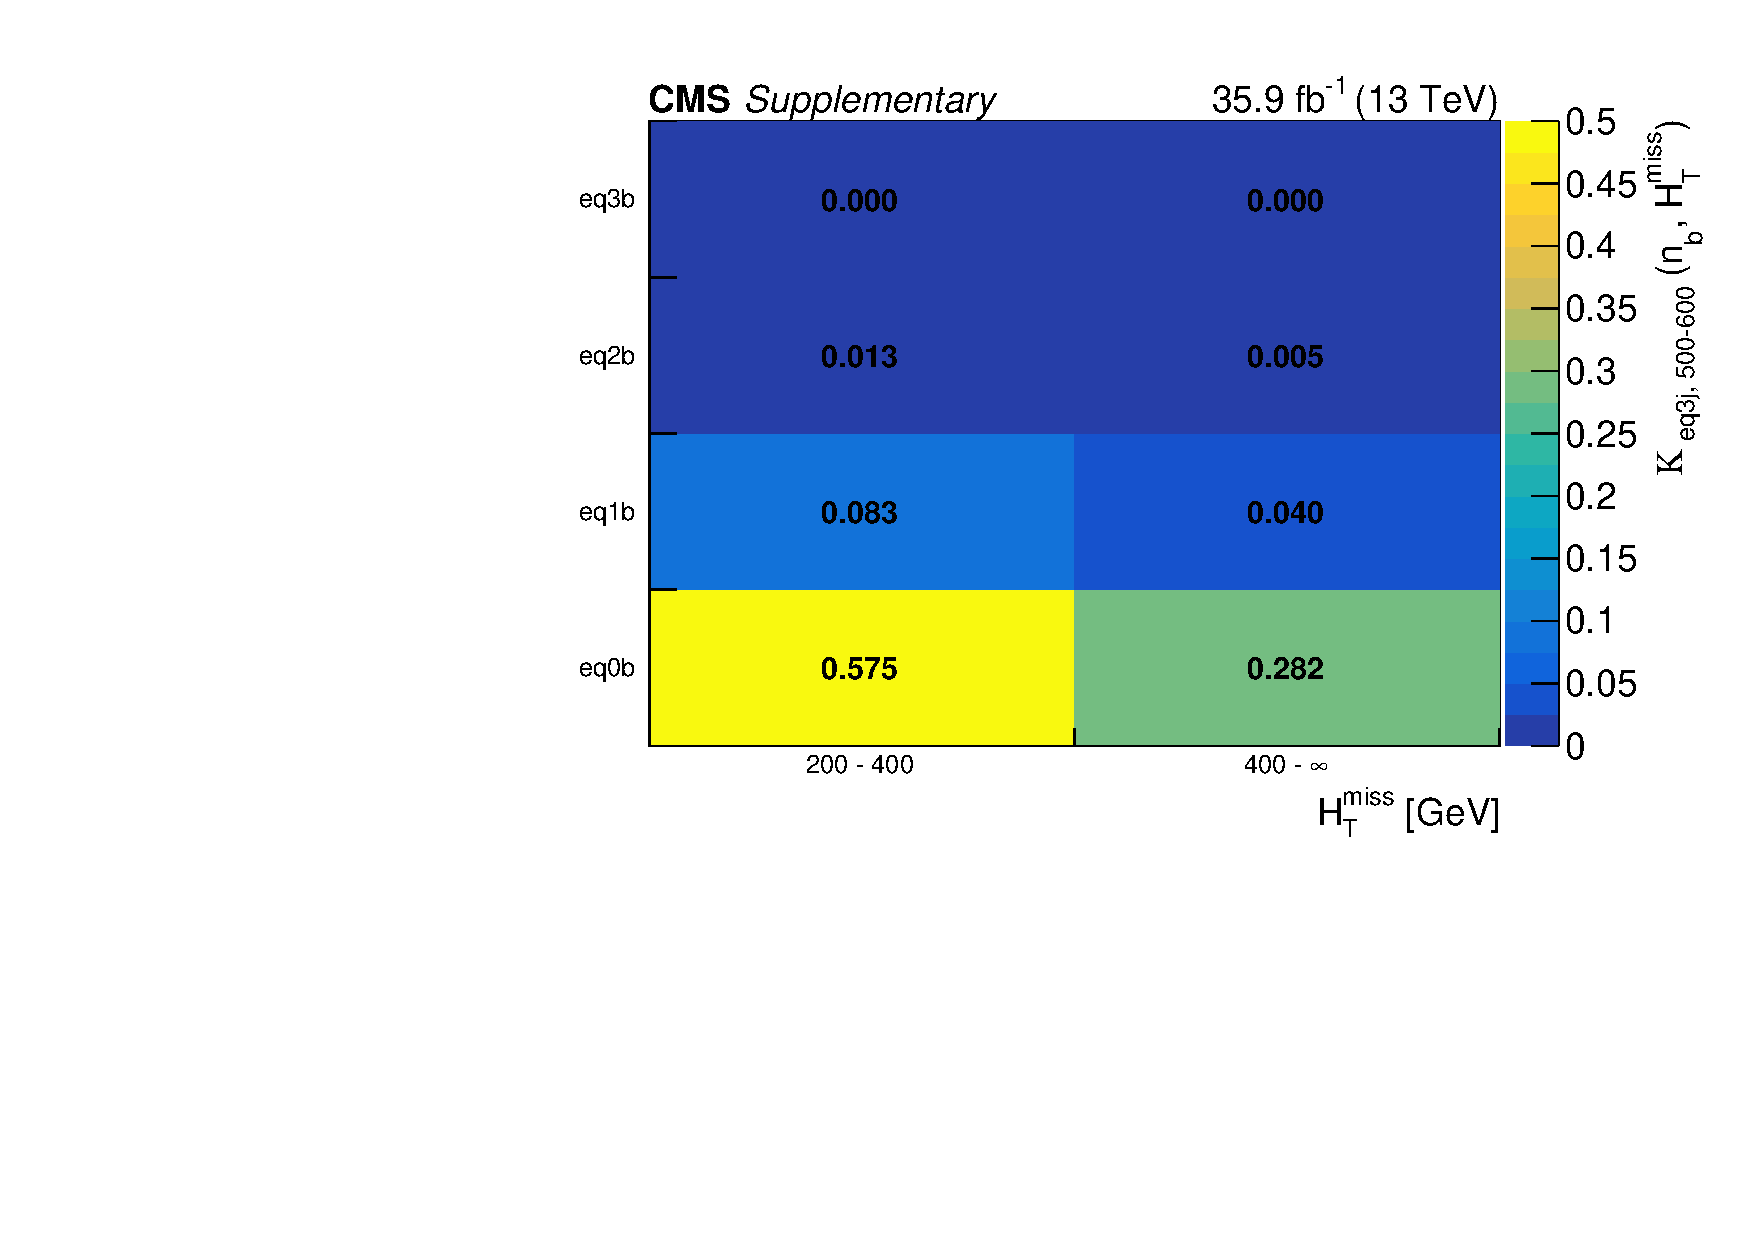
\includegraphics[width=0.3\textwidth]{figures/qcd/ewk_kappas/ewkKappa_eq3j_500-600}
    } \\
    \subfigure[$600<\scalht<750$ \gev]{
        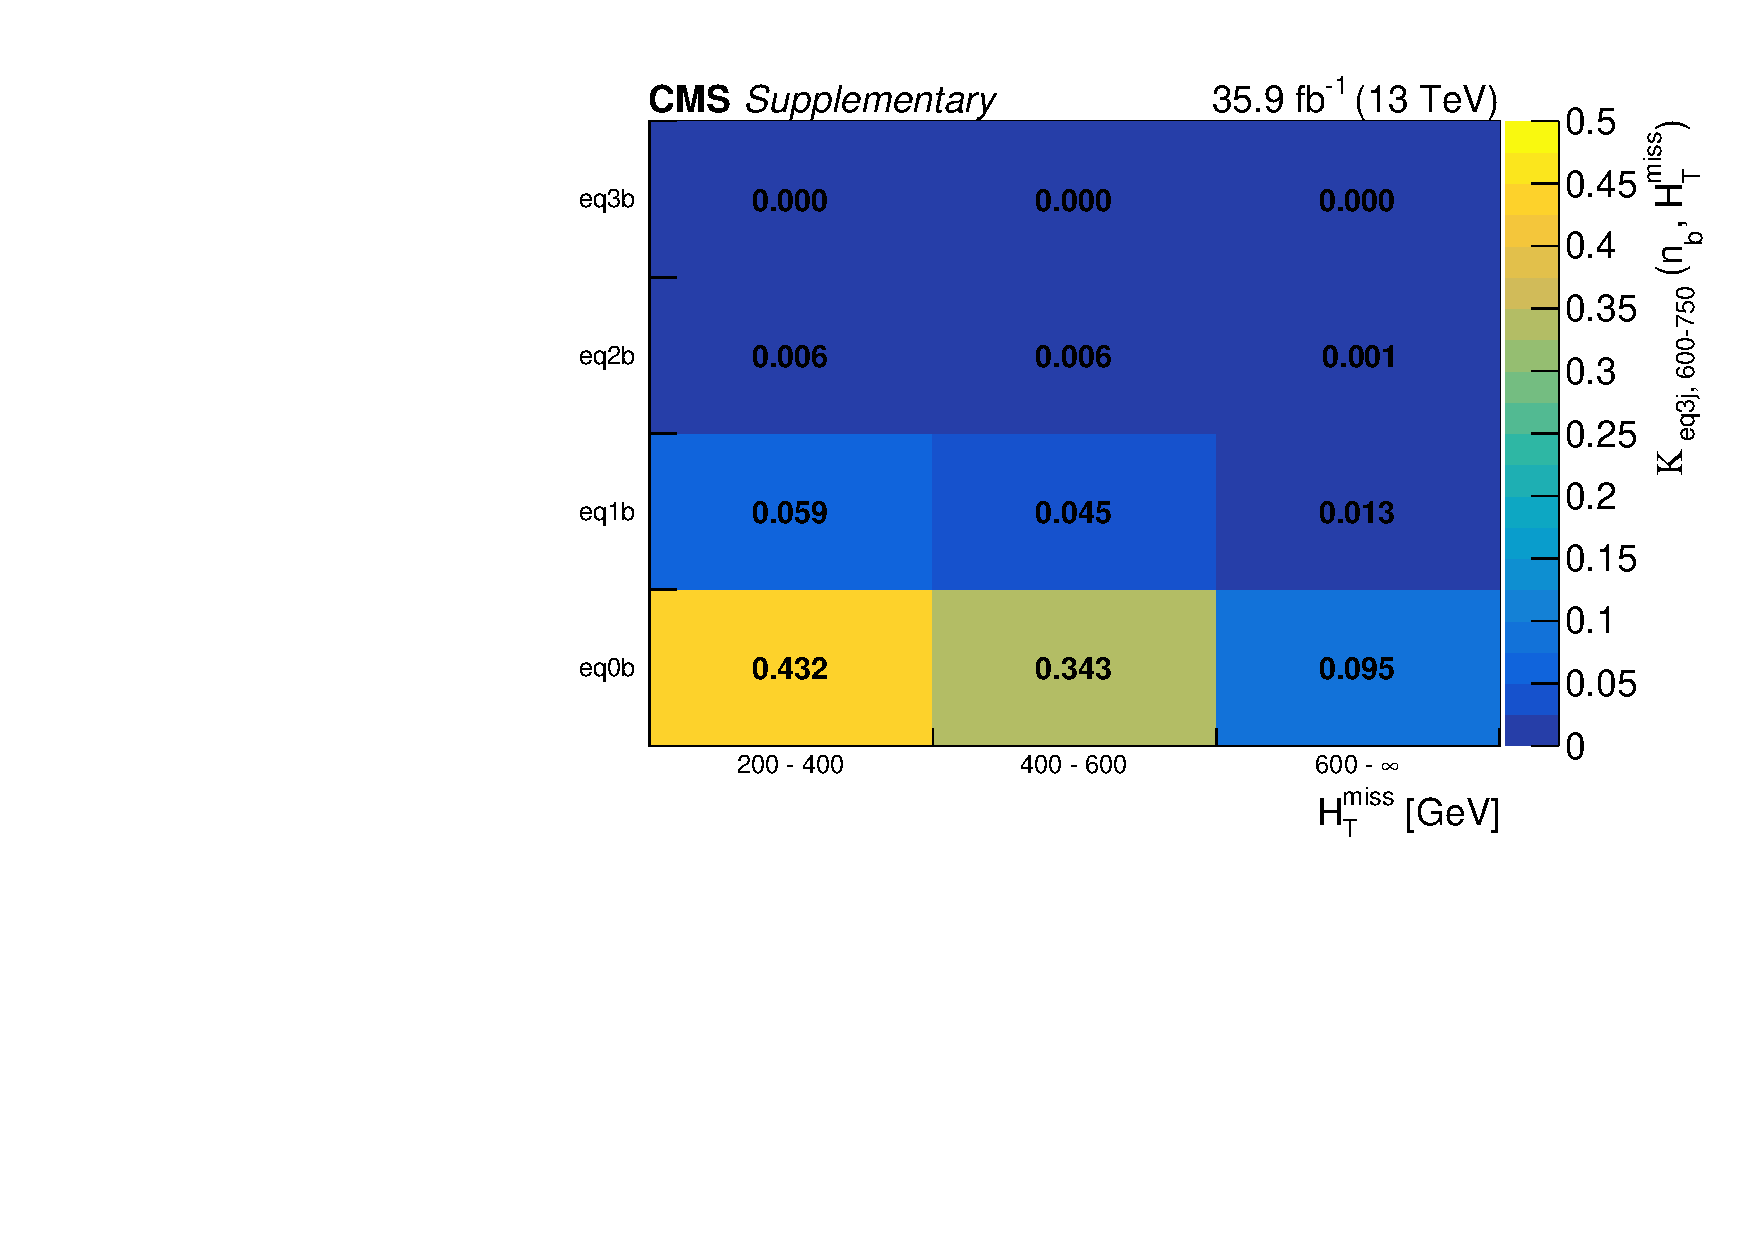
\includegraphics[width=0.3\textwidth]{figures/qcd/ewk_kappas/ewkKappa_eq3j_600-750}
    } ~~
    \subfigure[$750<\scalht<900$ \gev]{
        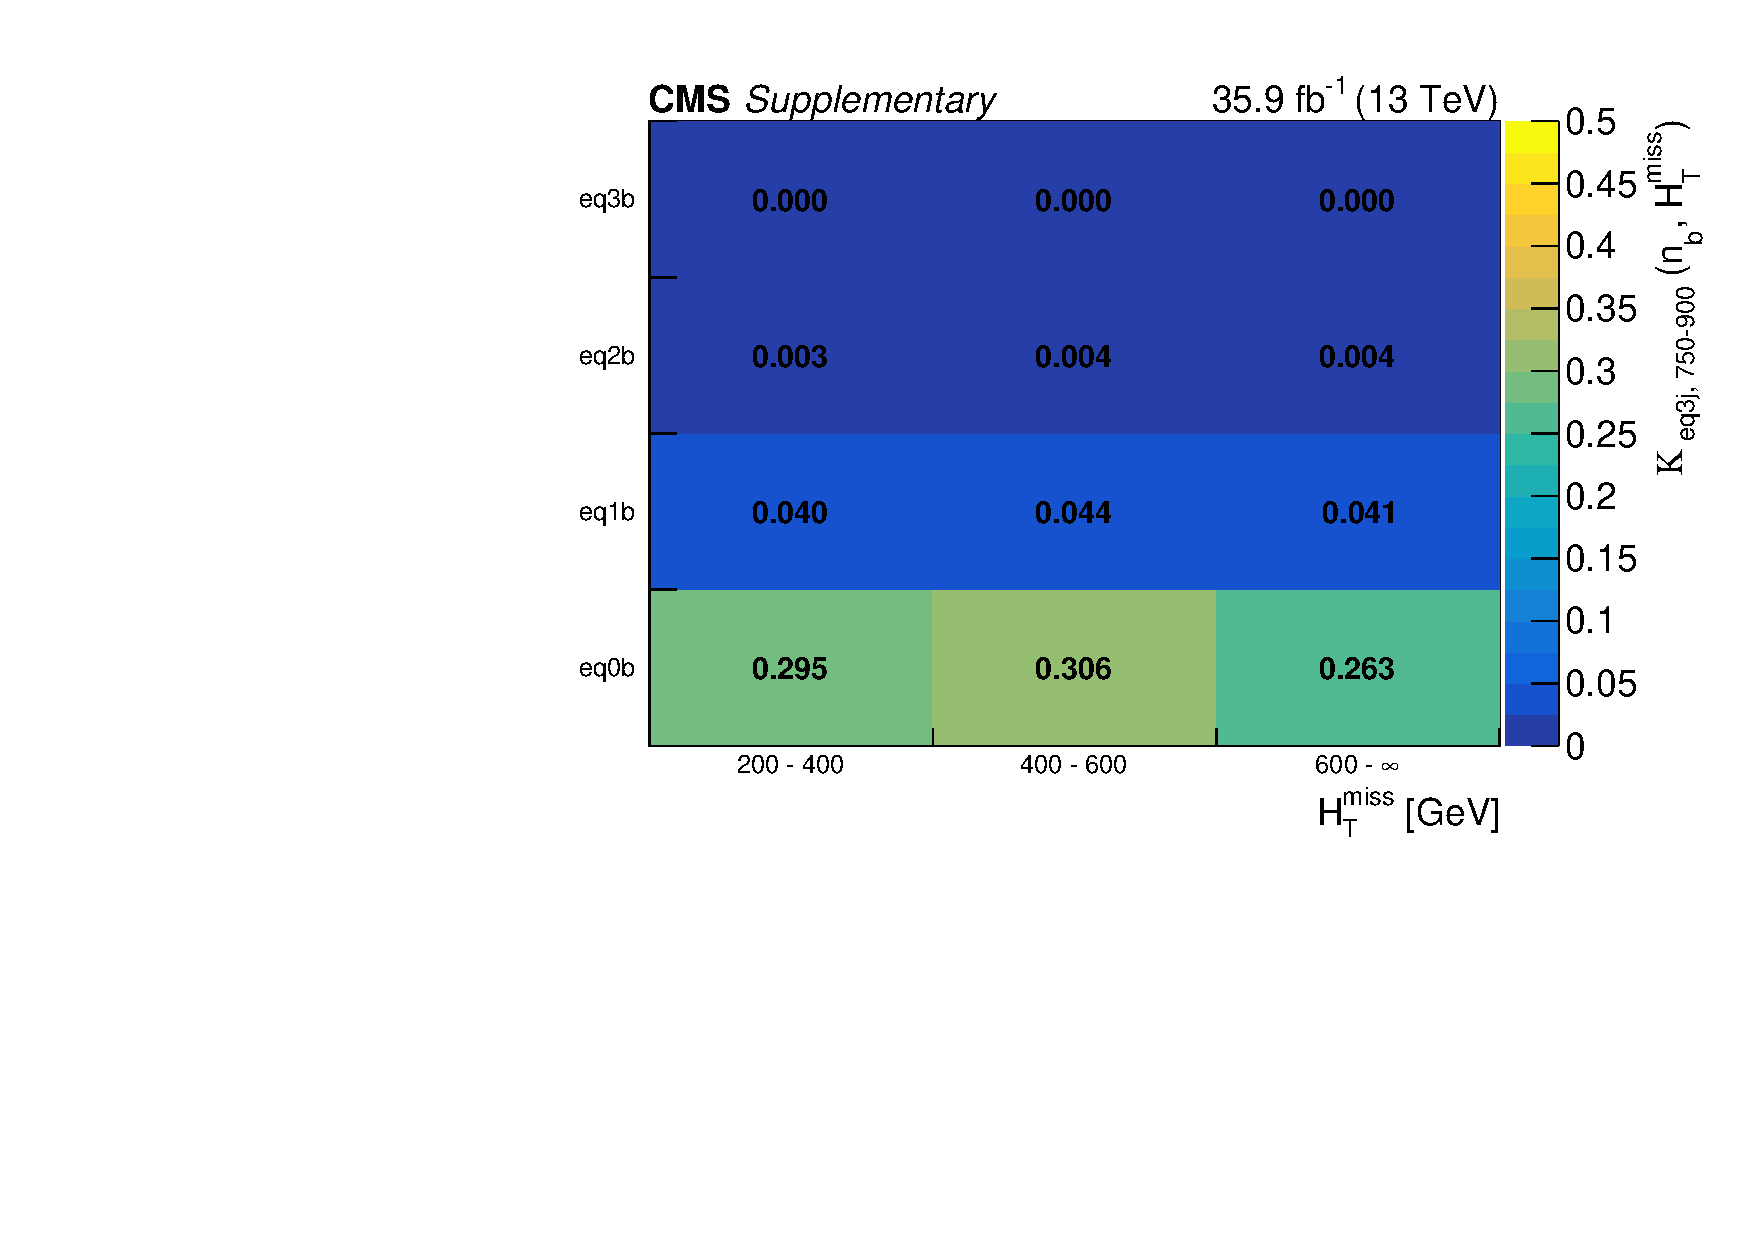
\includegraphics[width=0.3\textwidth]{figures/qcd/ewk_kappas/ewkKappa_eq3j_750-900}
    } ~~
    \subfigure[$900<\scalht<1050$ \gev]{
        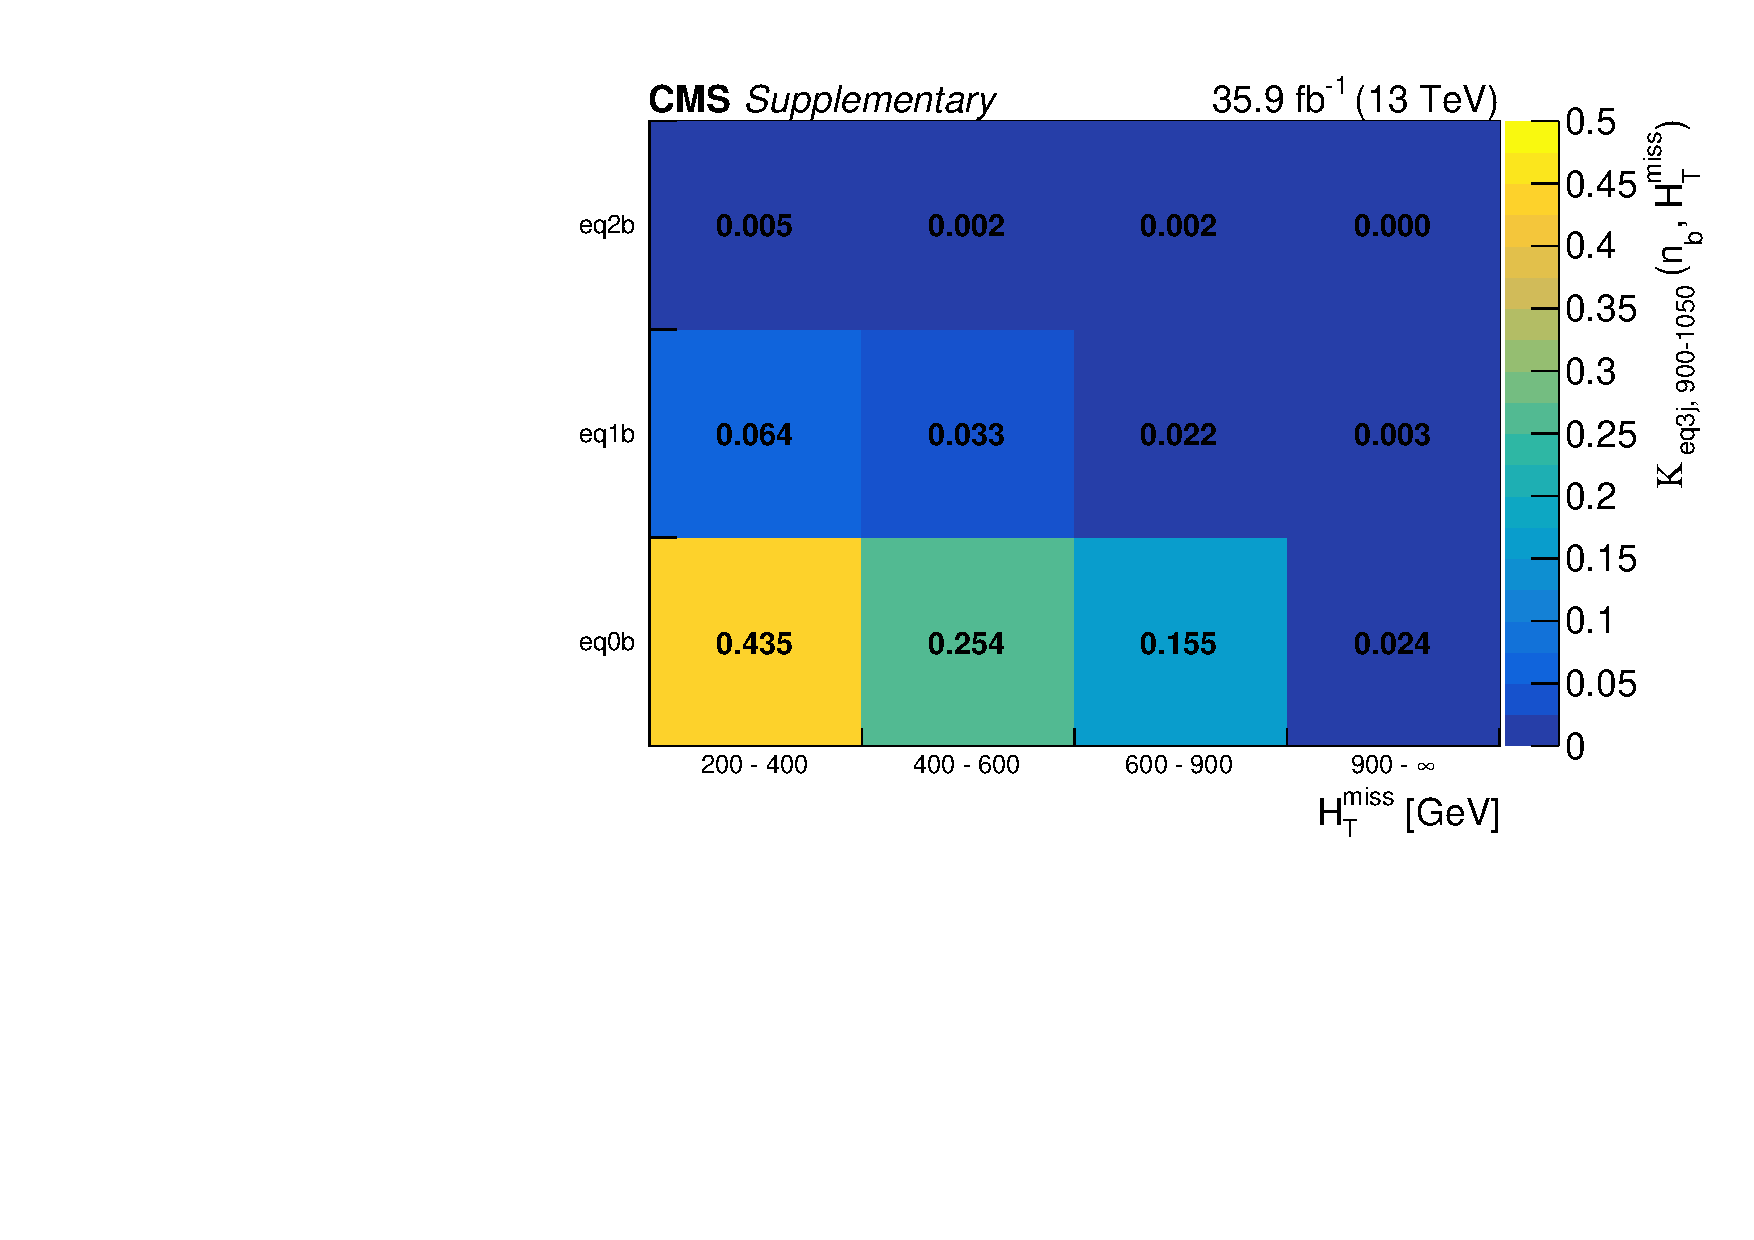
\includegraphics[width=0.3\textwidth]{figures/qcd/ewk_kappas/ewkKappa_eq3j_900-1050}
    } \\
    \subfigure[$1050<\scalht<1200$ \gev]{
        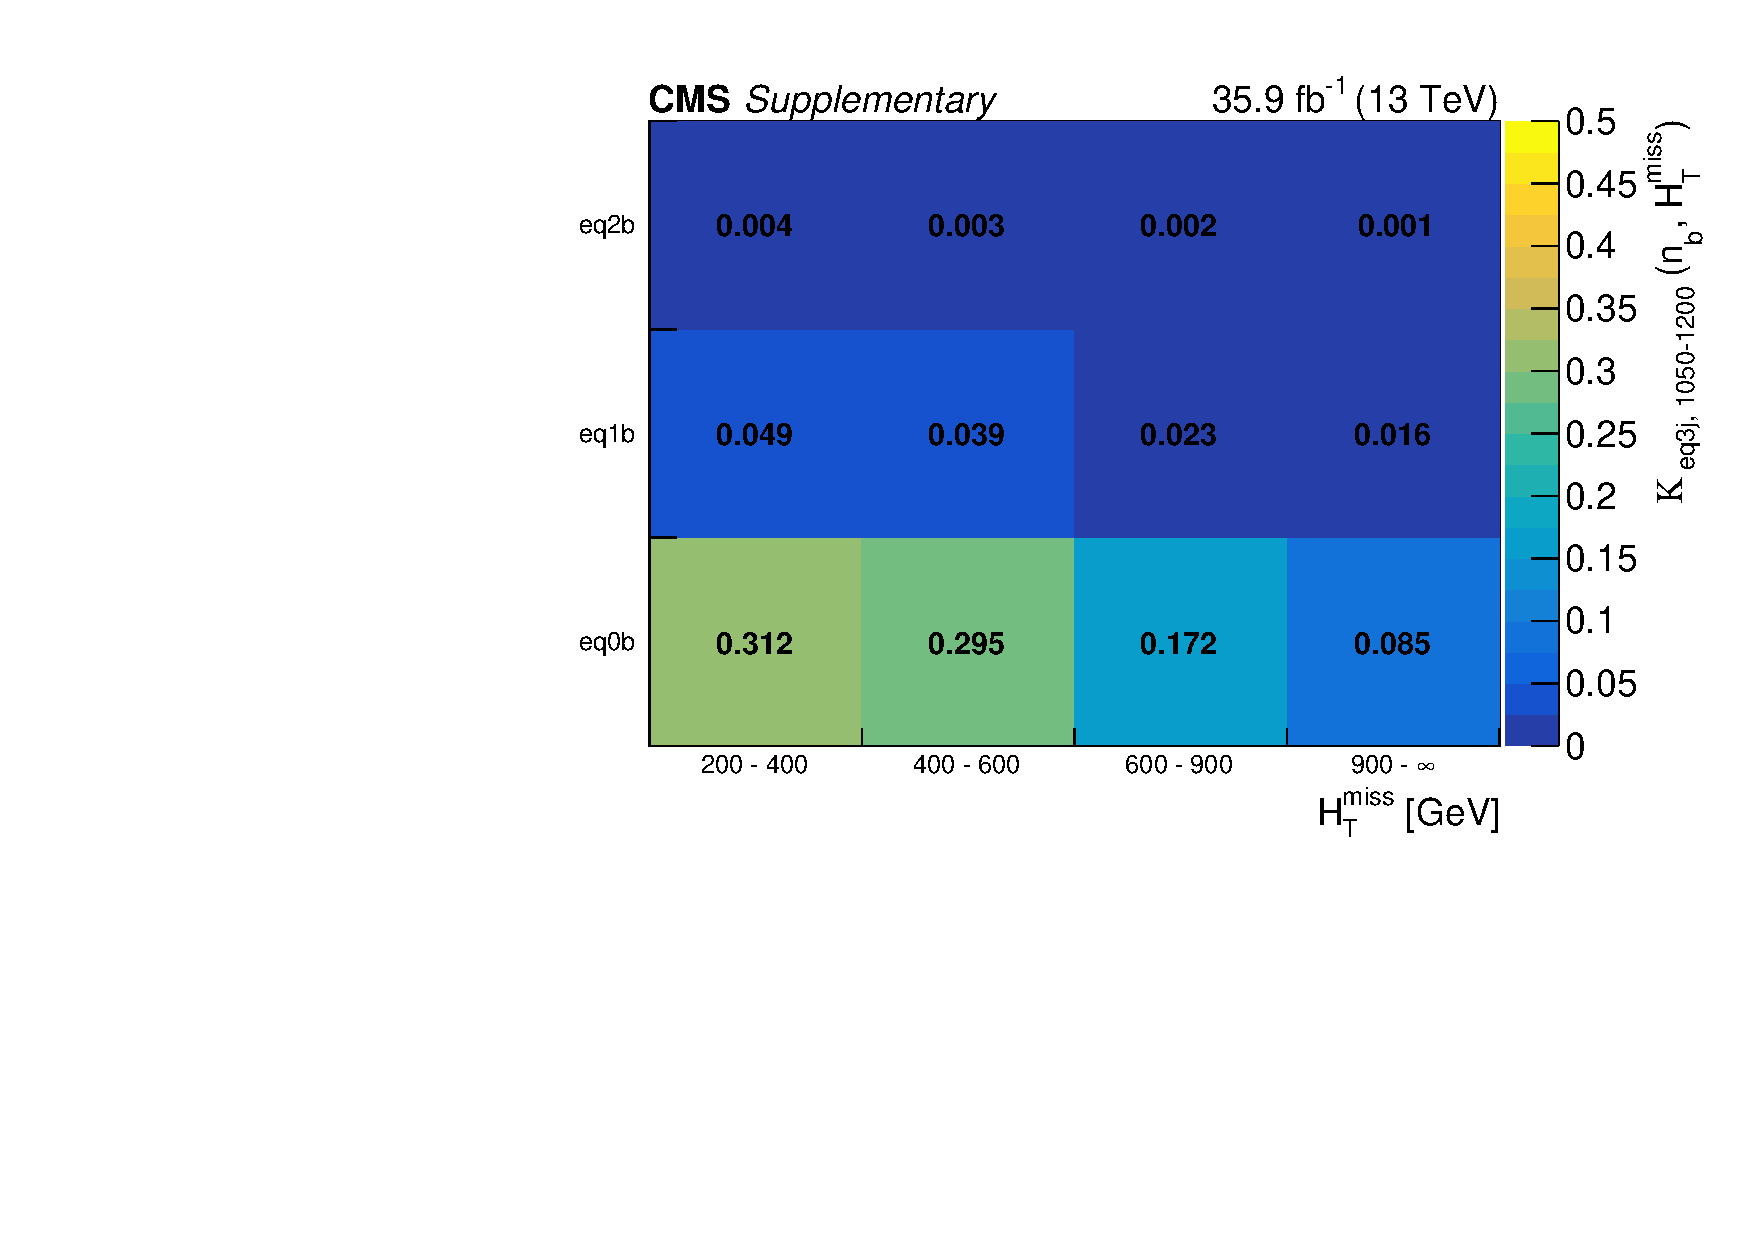
\includegraphics[width=0.3\textwidth]{figures/qcd/ewk_kappas/ewkKappa_eq3j_1050-1200}
    } ~~
    \subfigure[$900<\scalht<\infty$ \gev]{
        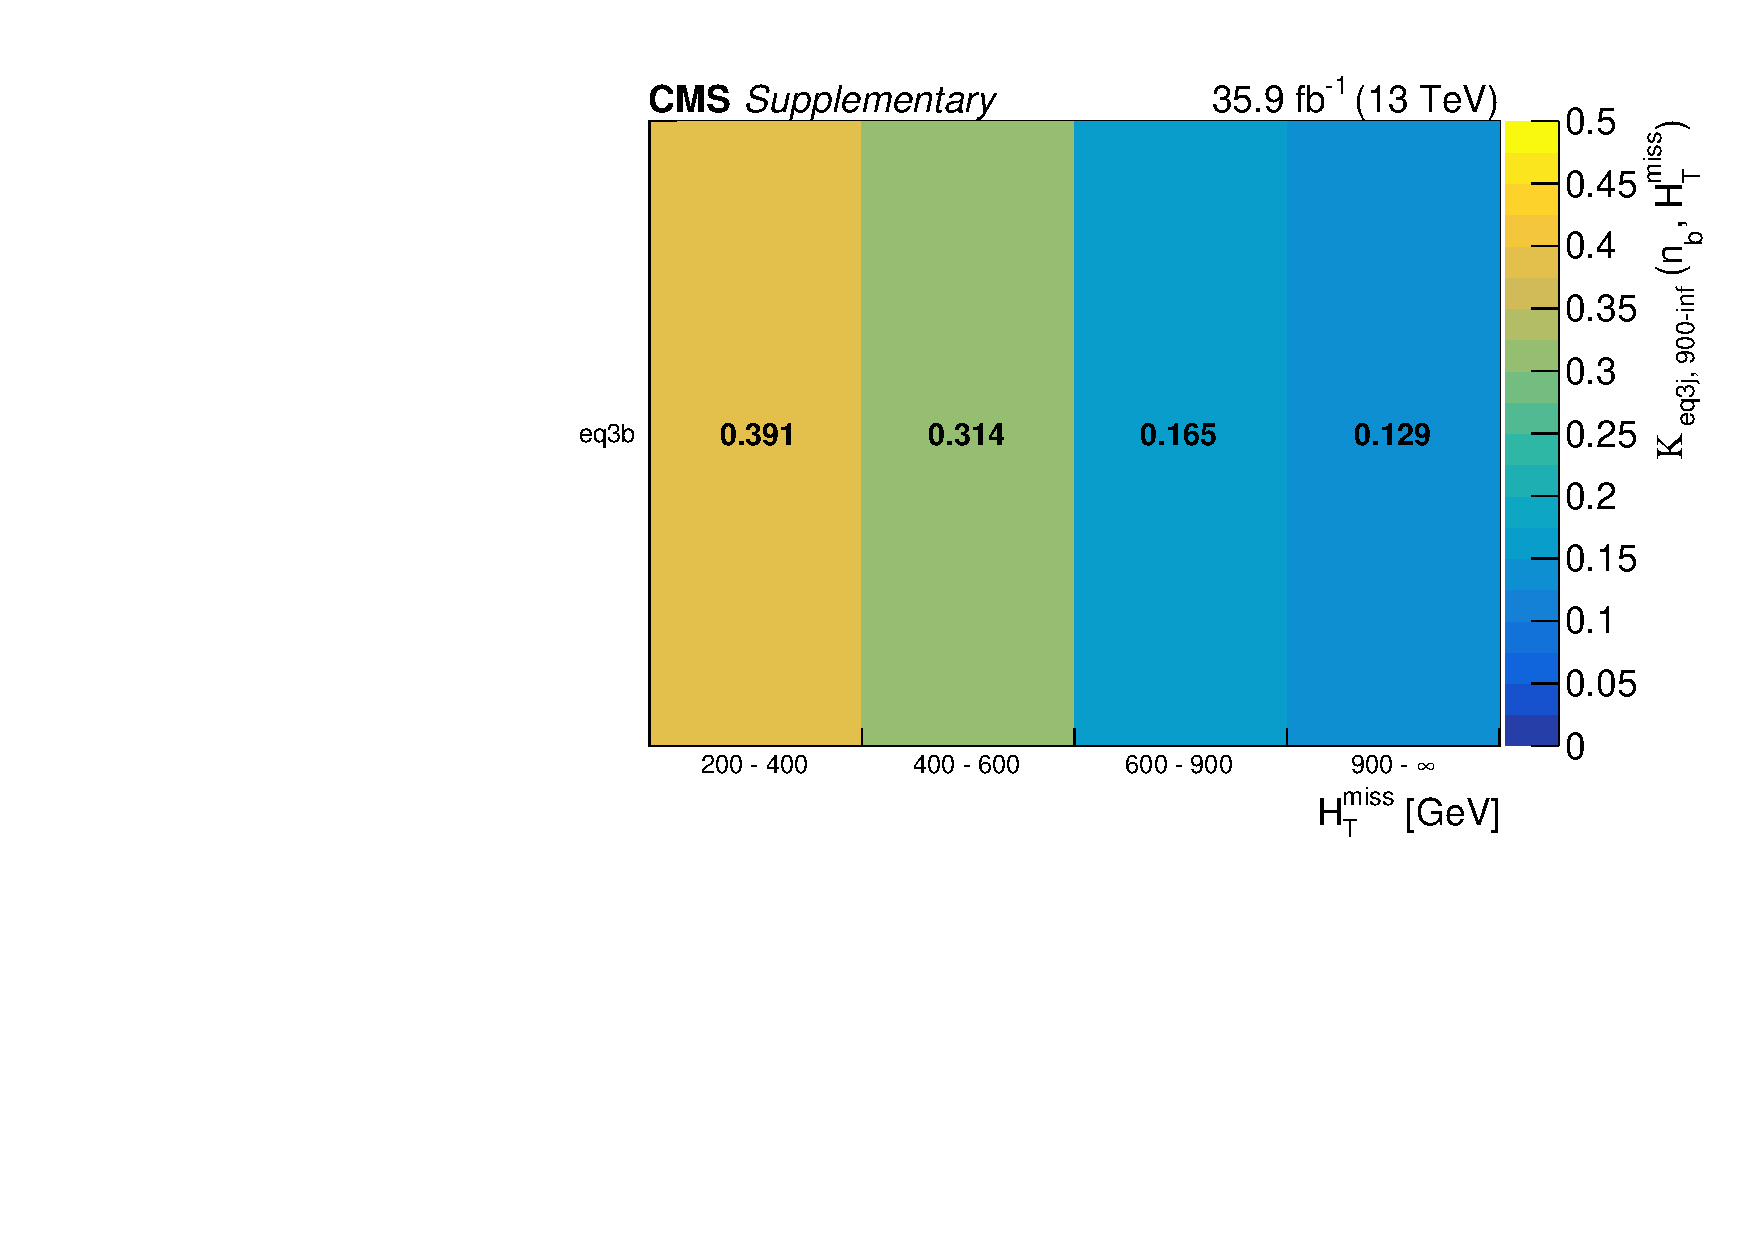
\includegraphics[width=0.3\textwidth]{figures/qcd/ewk_kappas/ewkKappa_eq3j_900-inf}
    } ~~
    \subfigure[$1200<\scalht<\infty$ \gev]{
        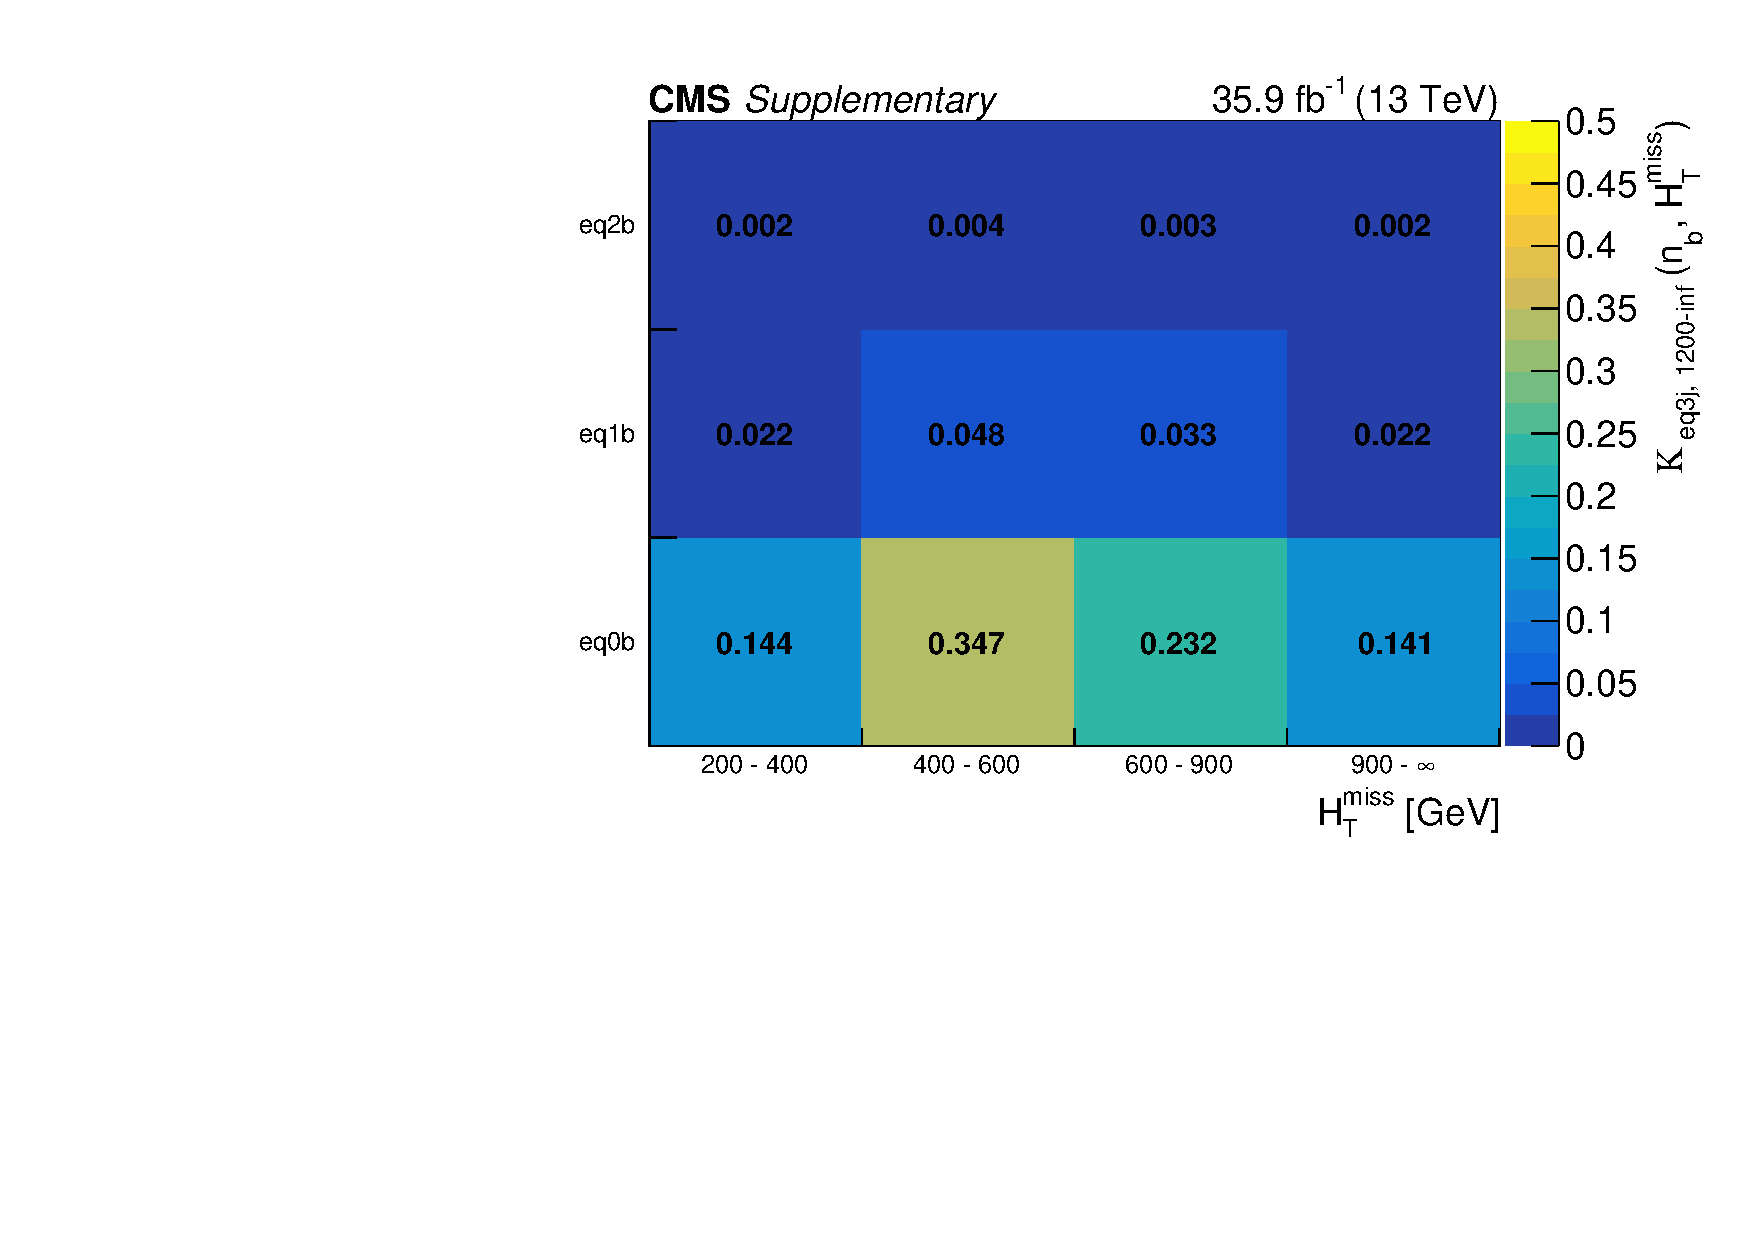
\includegraphics[width=0.3\textwidth]{figures/qcd/ewk_kappas/ewkKappa_eq3j_1200-inf}
    } \\
    \caption{
        Electroweak (\ttw) eq3j kappa factors used to distribute
        the QCD multijet prediction across the \nb and \mht dimensions.
    }
    \label{fig:ewk_kappas_eq3j}
\end{figure}

\begin{figure}[!h]
    \centering
    \subfigure[$400<\scalht<500$ \gev]{
        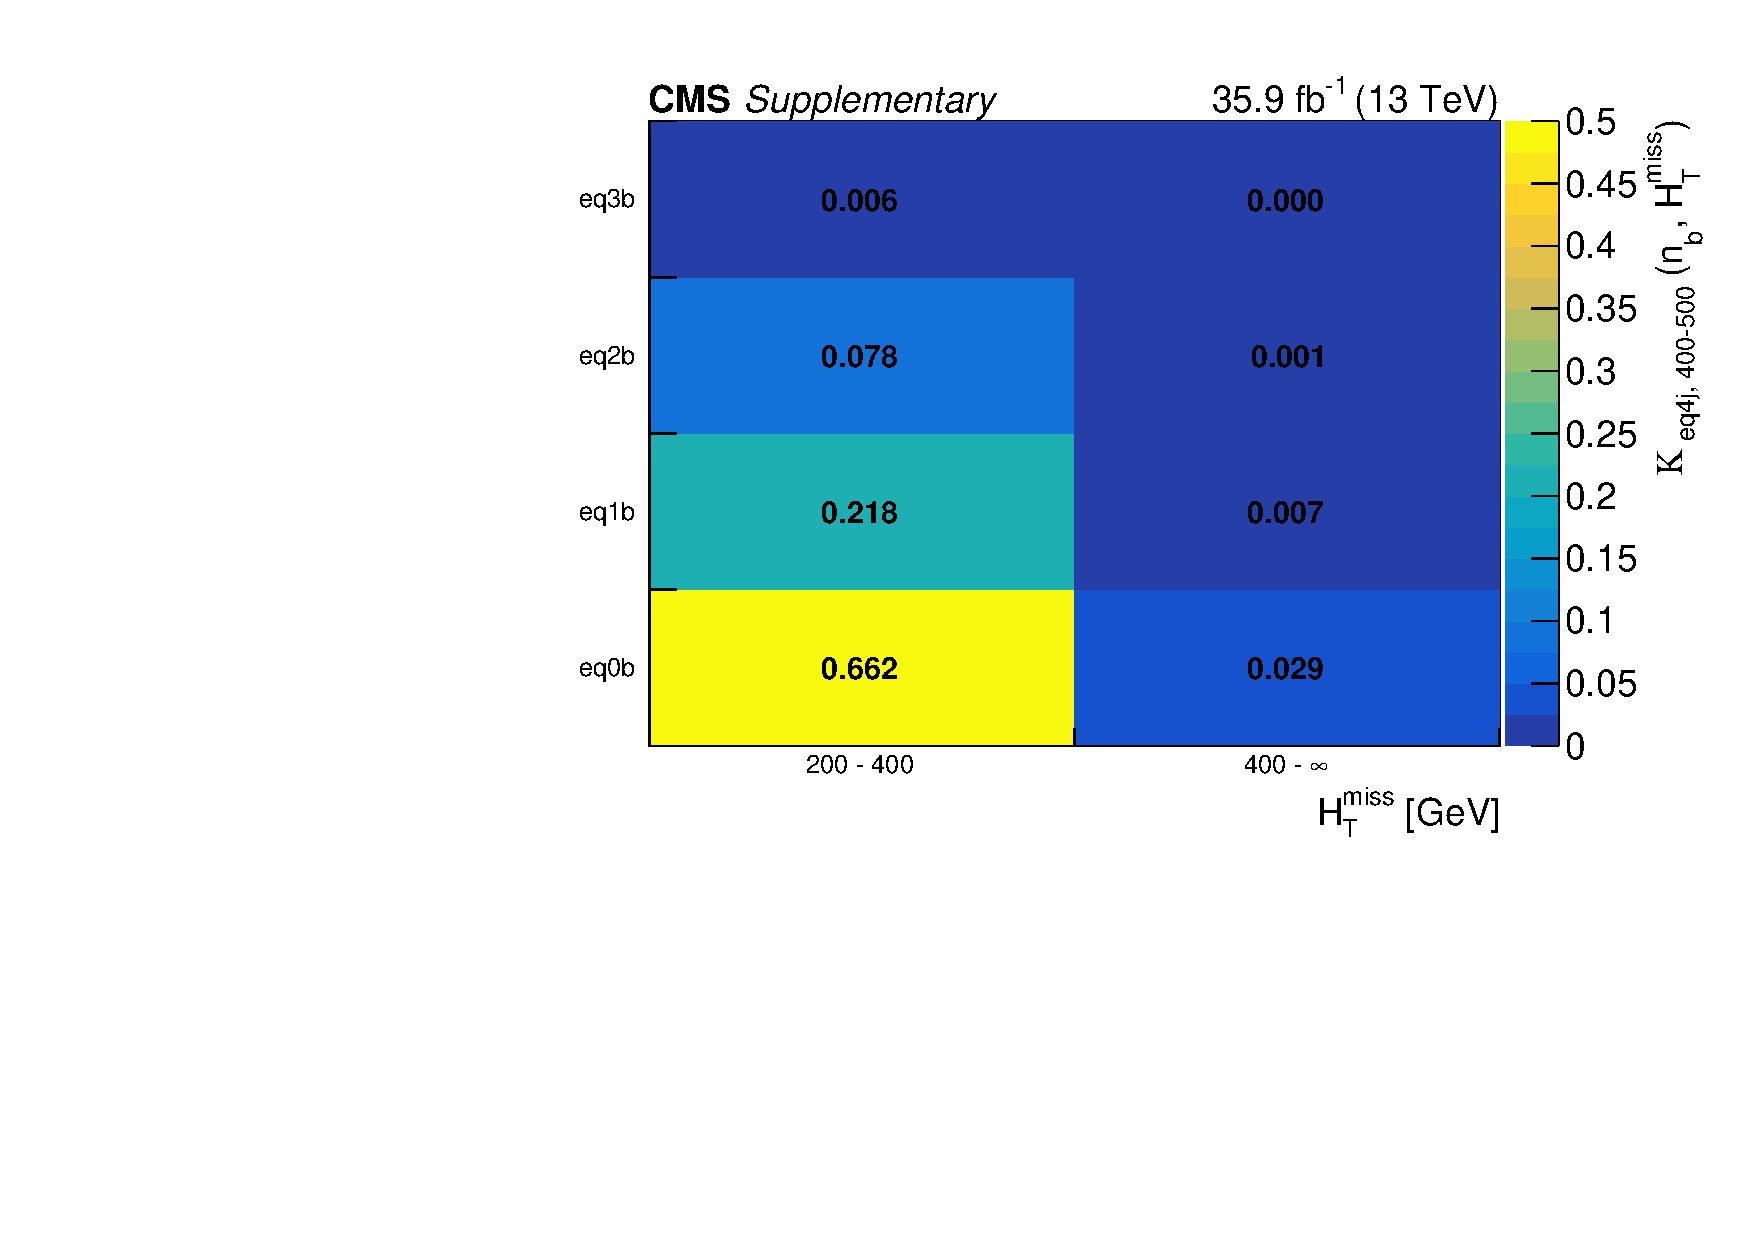
\includegraphics[width=0.3\textwidth]{figures/qcd/ewk_kappas/ewkKappa_eq4j_400-500}
    } ~~
    \subfigure[$500<\scalht<600$ \gev]{
        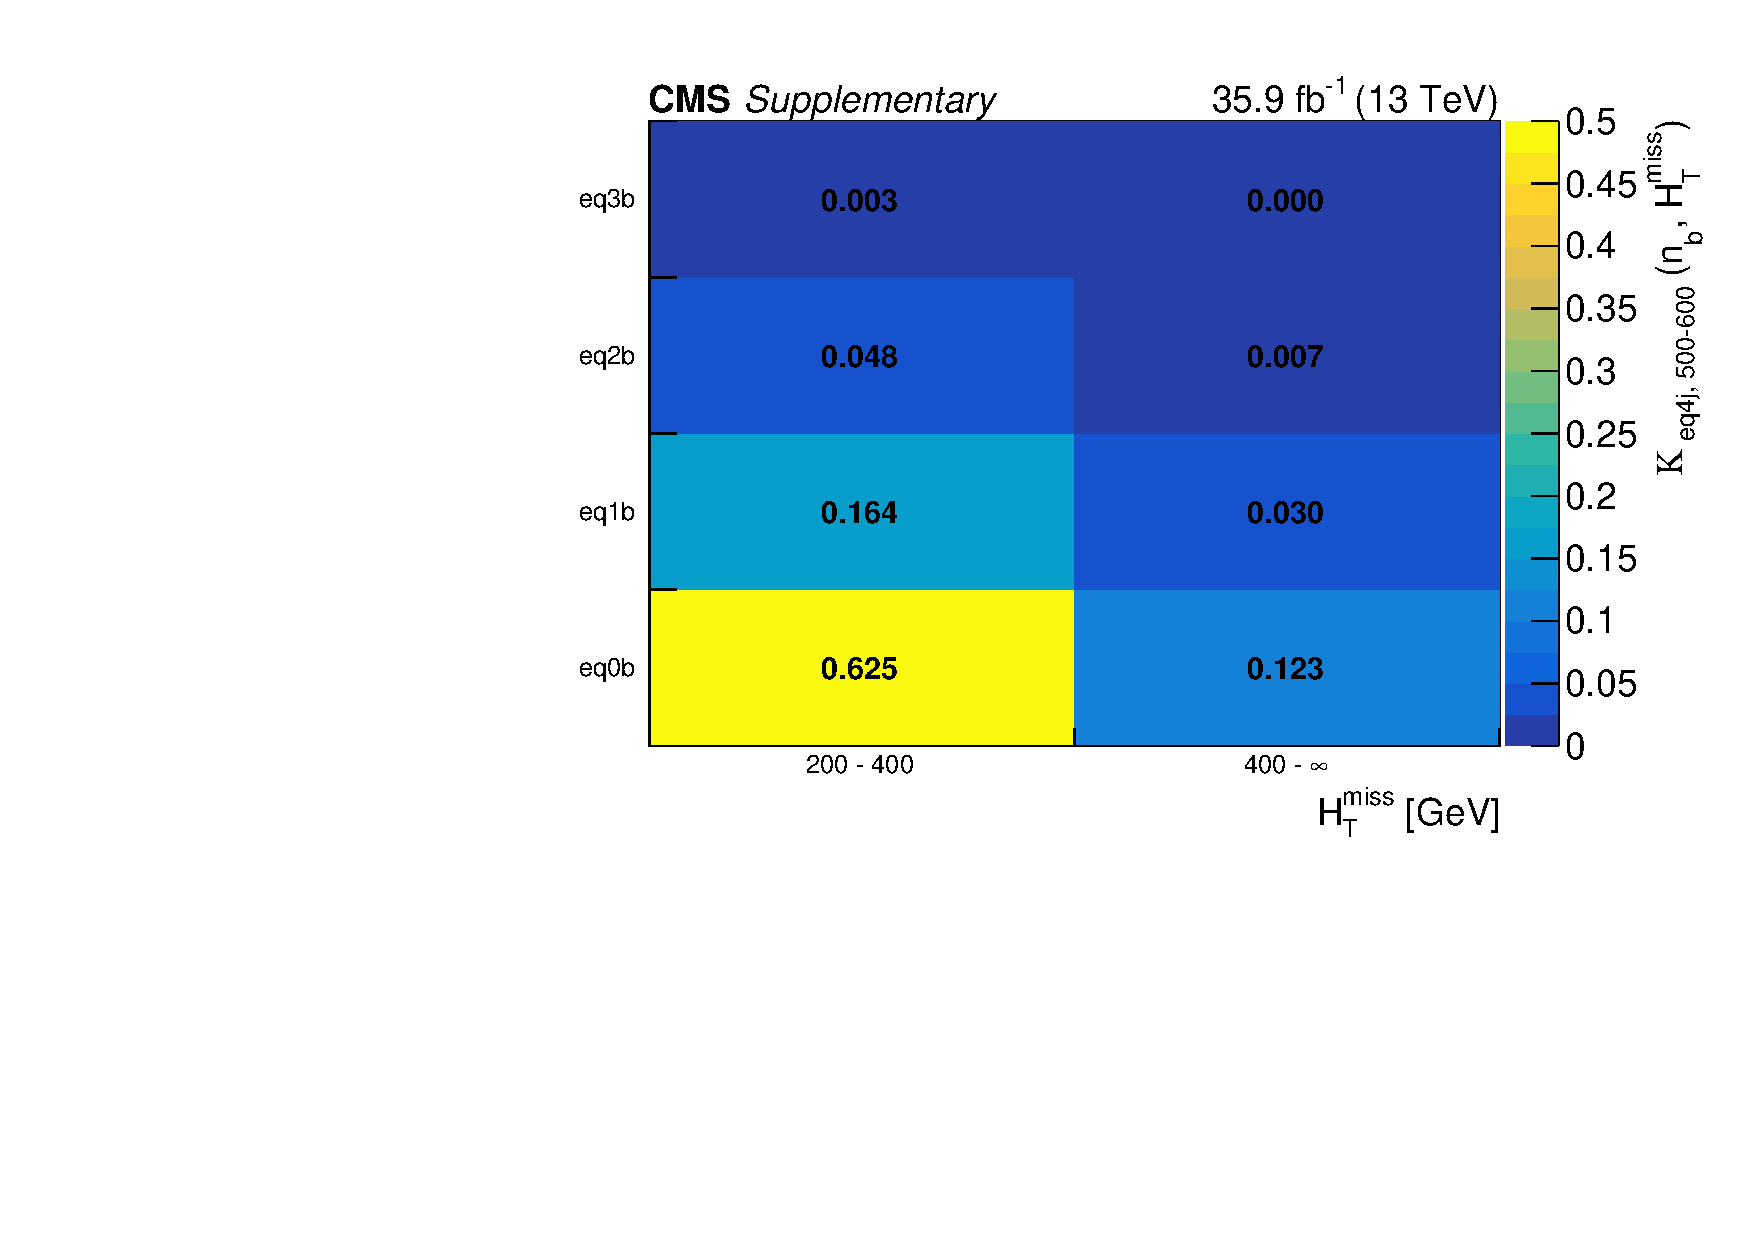
\includegraphics[width=0.3\textwidth]{figures/qcd/ewk_kappas/ewkKappa_eq4j_500-600}
    } ~~
    \subfigure[$600<\scalht<750$ \gev]{
        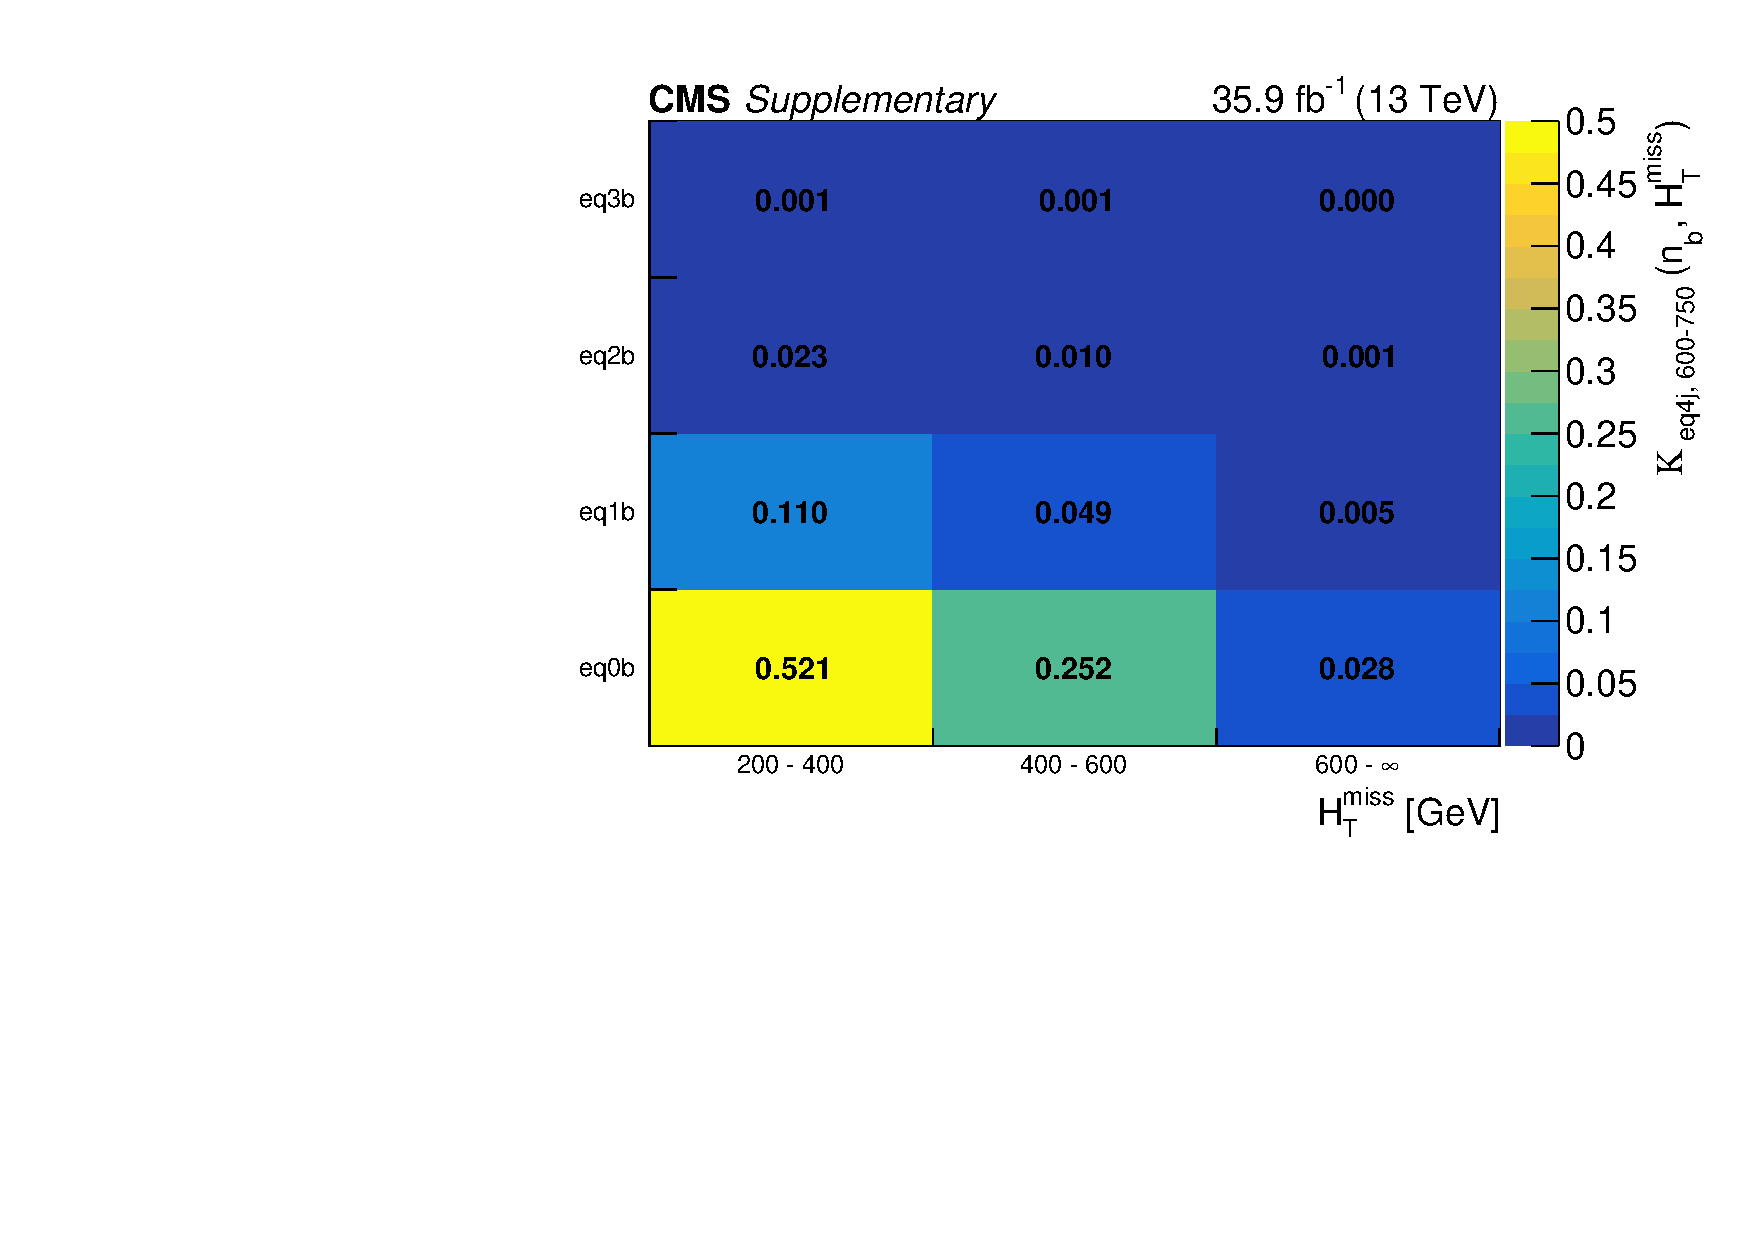
\includegraphics[width=0.3\textwidth]{figures/qcd/ewk_kappas/ewkKappa_eq4j_600-750}
    } \\
    \subfigure[$750<\scalht<900$ \gev]{
        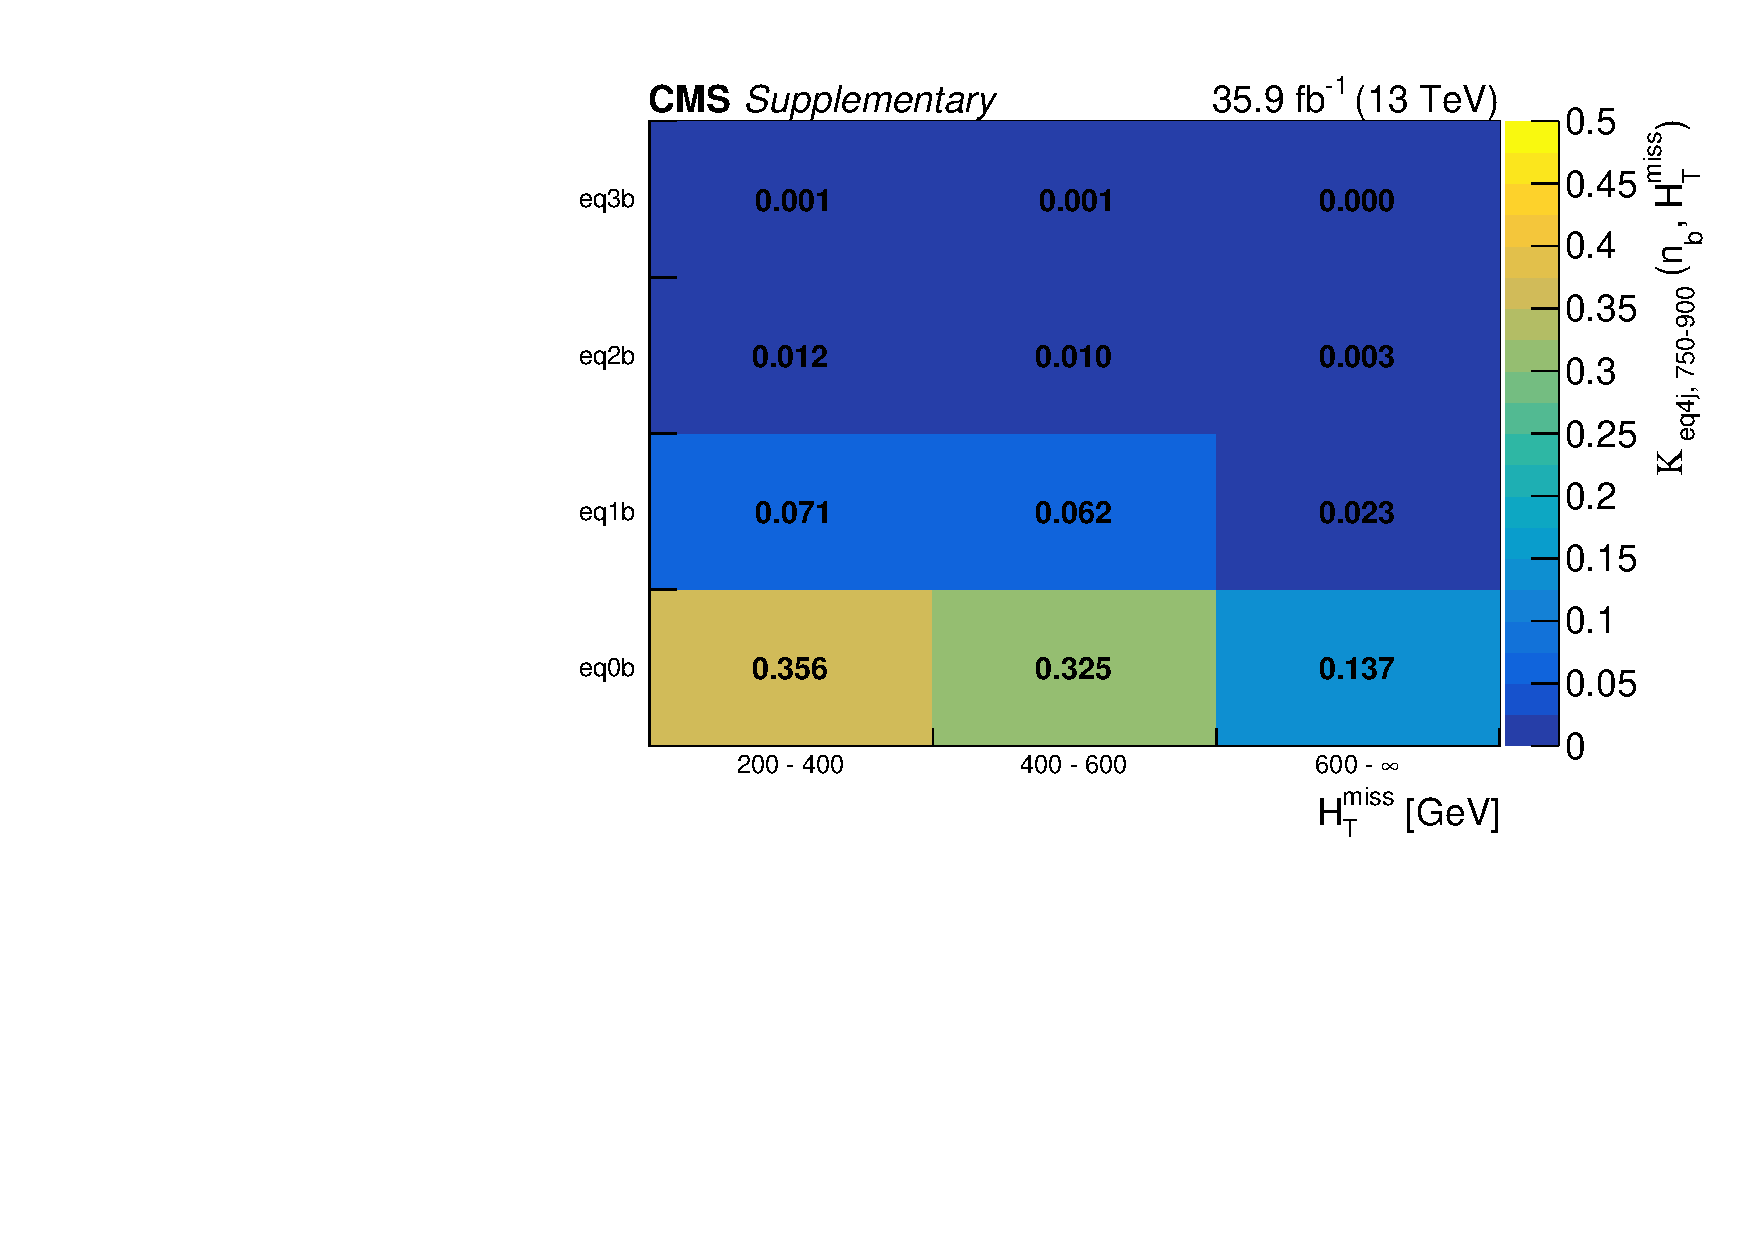
\includegraphics[width=0.3\textwidth]{figures/qcd/ewk_kappas/ewkKappa_eq4j_750-900}
    } ~~
    \subfigure[$900<\scalht<1050$ \gev]{
        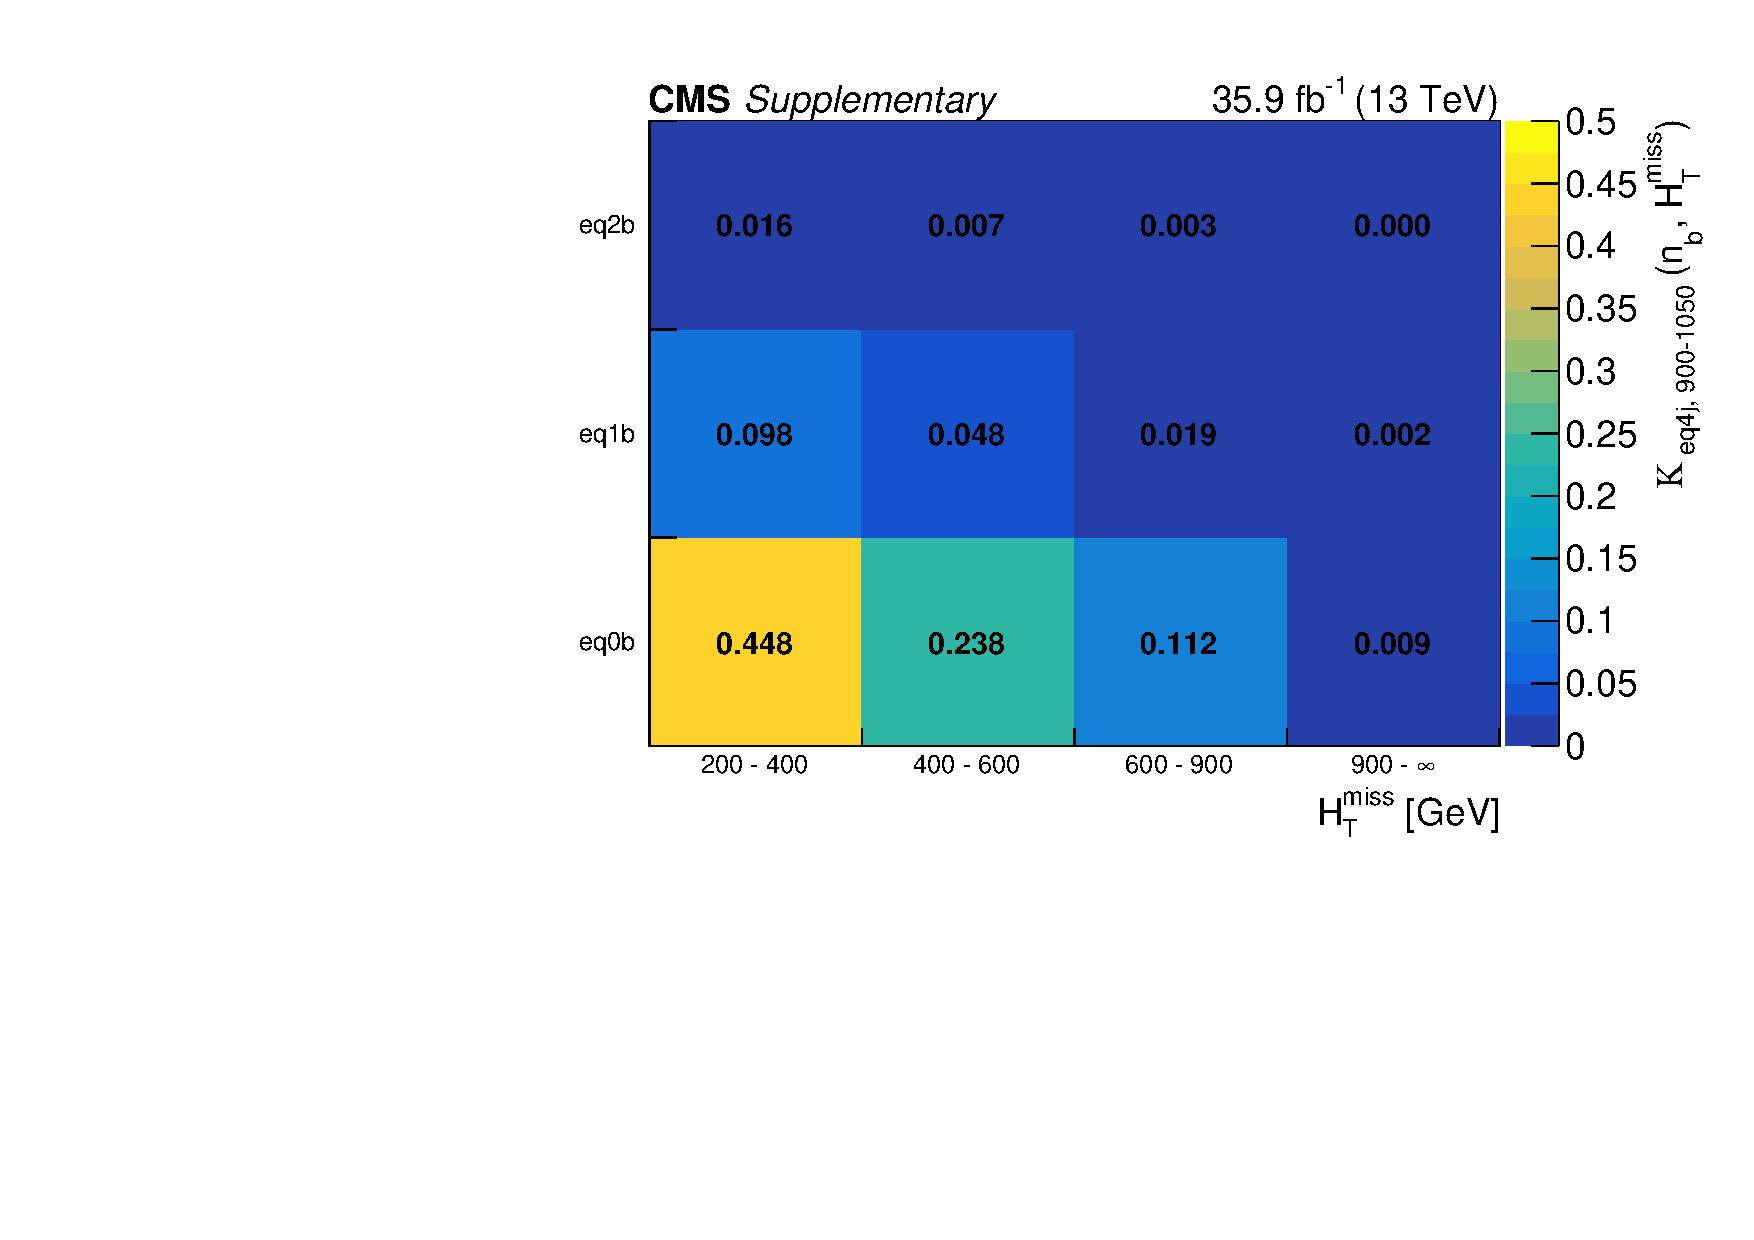
\includegraphics[width=0.3\textwidth]{figures/qcd/ewk_kappas/ewkKappa_eq4j_900-1050}
    } ~~
    \subfigure[$1050<\scalht<1200$ \gev]{
        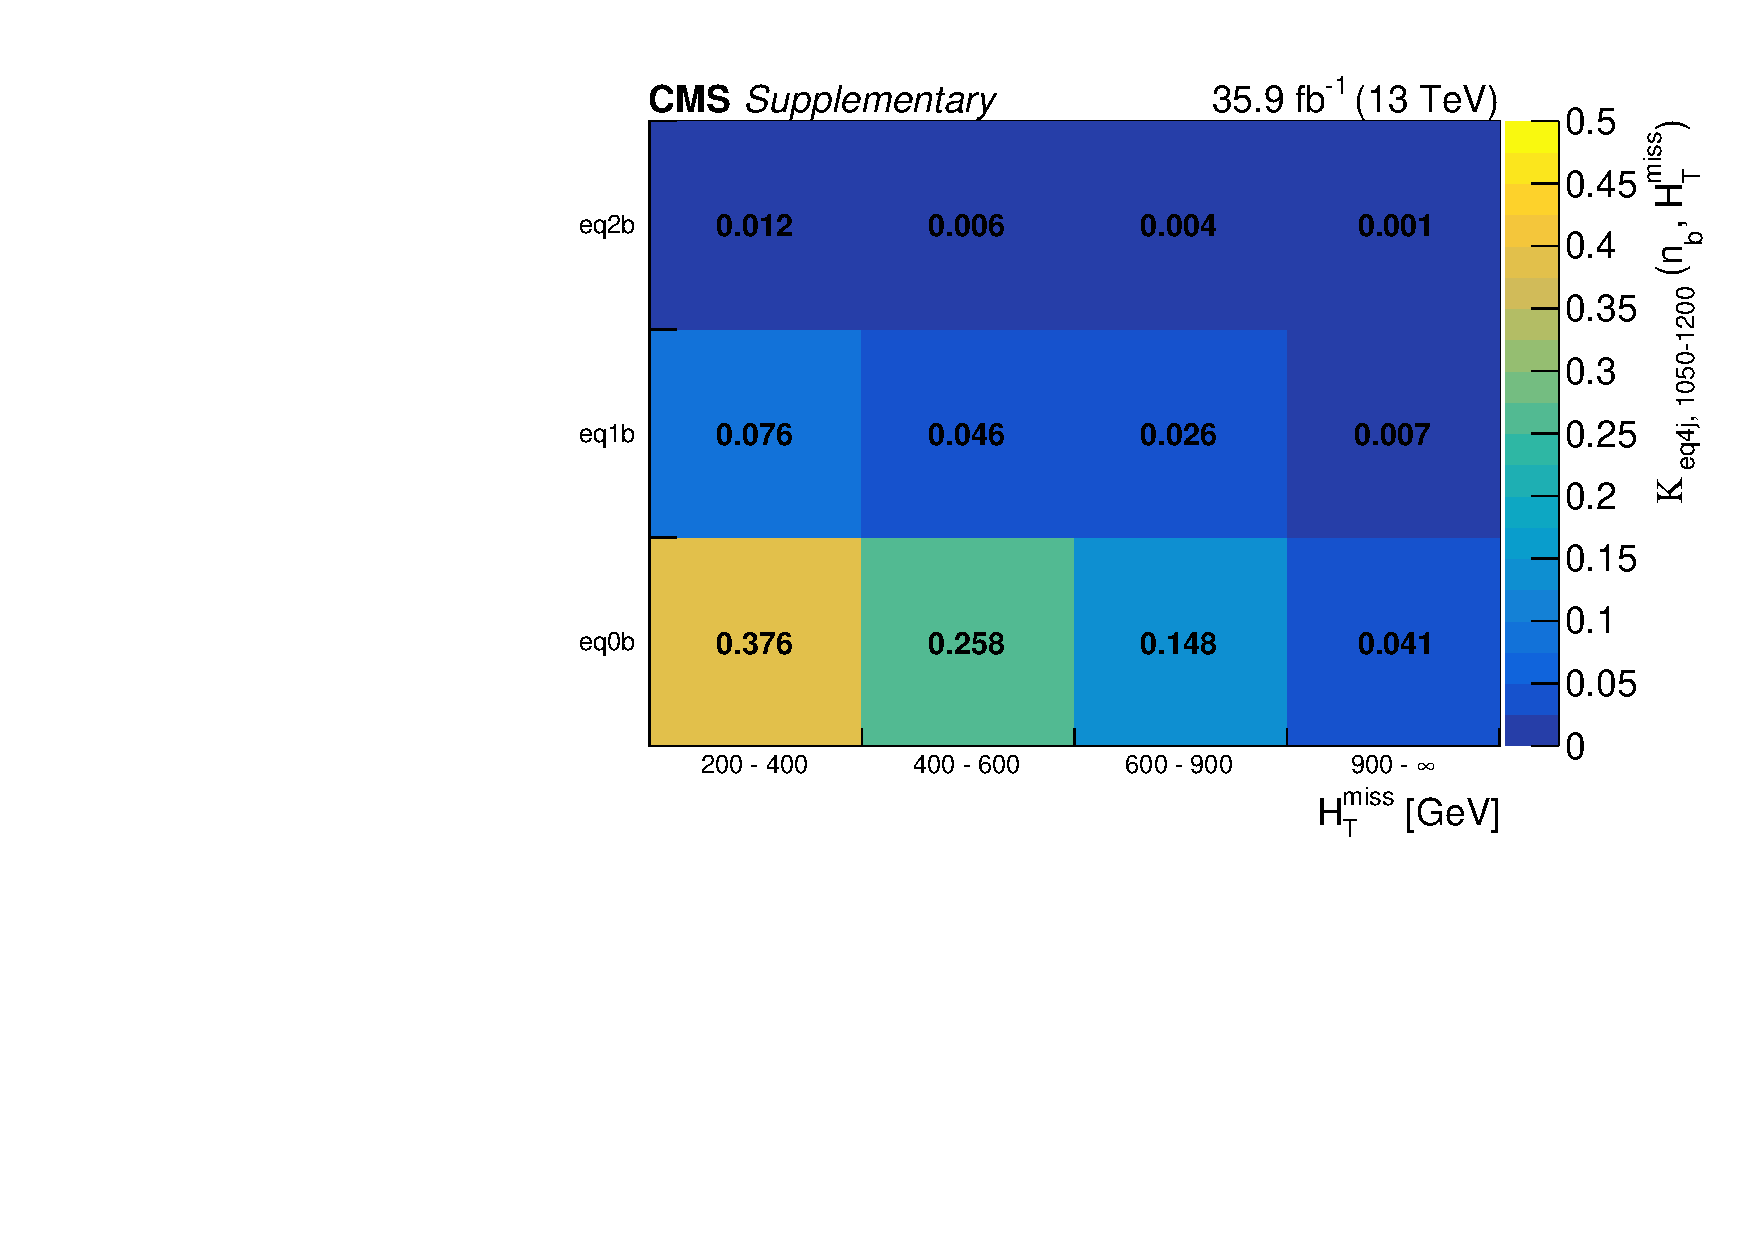
\includegraphics[width=0.3\textwidth]{figures/qcd/ewk_kappas/ewkKappa_eq4j_1050-1200}
    } \\
    \subfigure[$900<\scalht<\infty$ \gev]{
        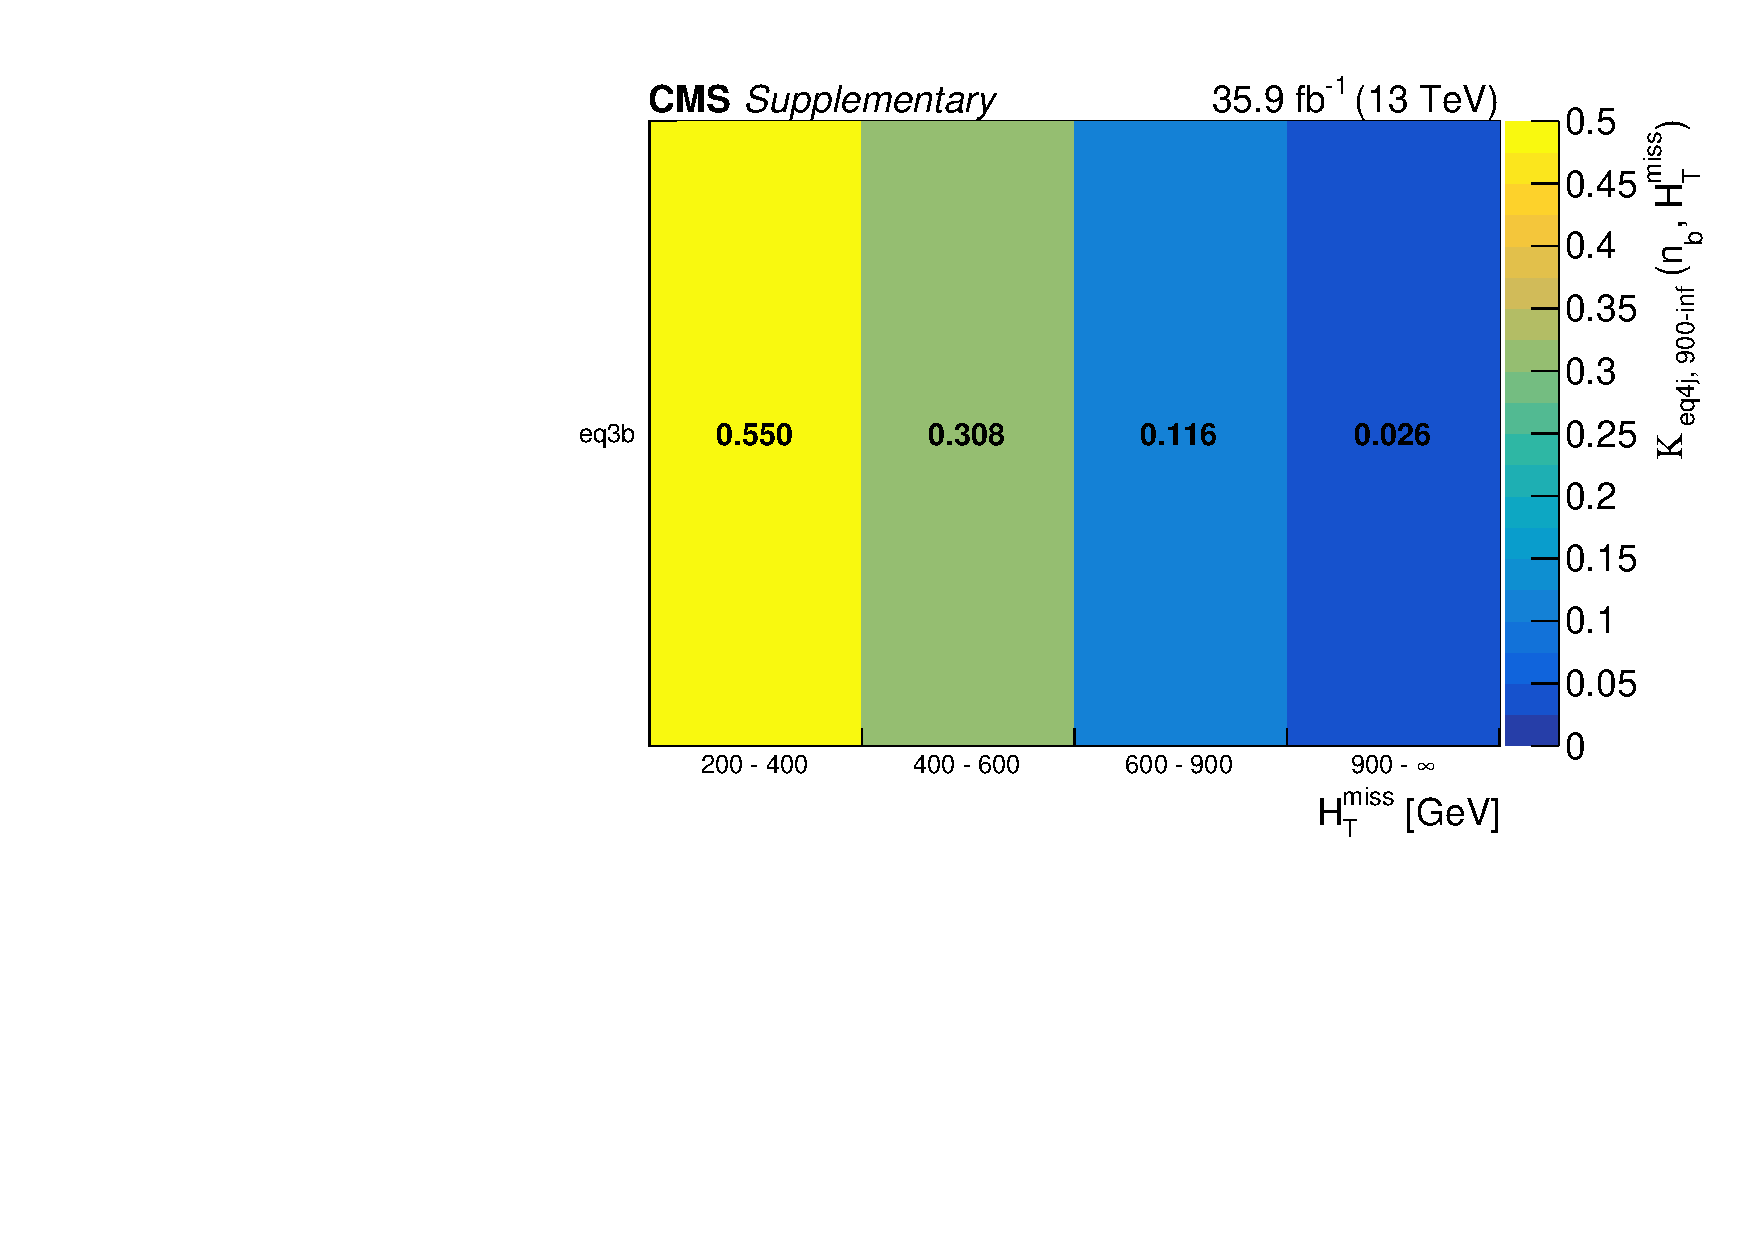
\includegraphics[width=0.3\textwidth]{figures/qcd/ewk_kappas/ewkKappa_eq4j_900-inf}
    } ~~
    \subfigure[$1200<\scalht<\infty$ \gev]{
        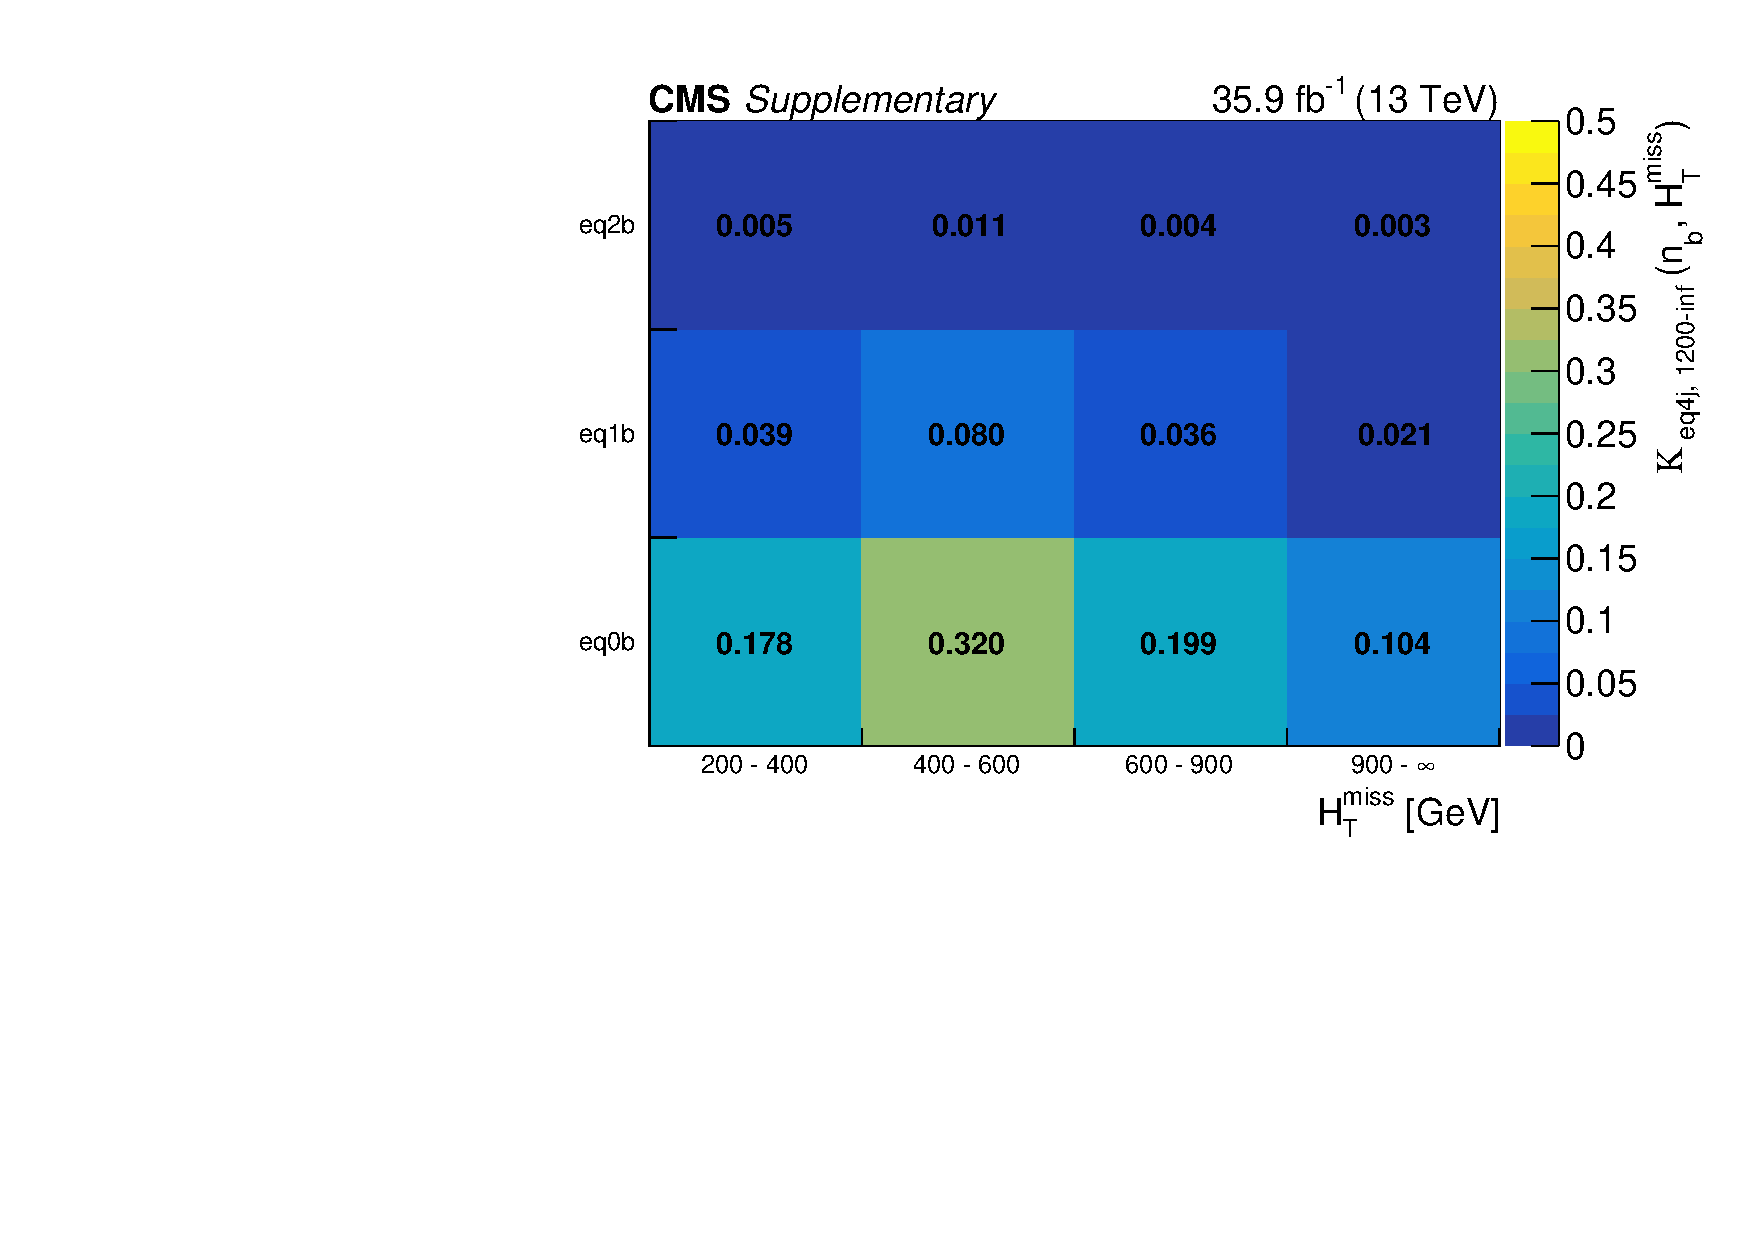
\includegraphics[width=0.3\textwidth]{figures/qcd/ewk_kappas/ewkKappa_eq4j_1200-inf}
    } ~~
    \caption{
        Electroweak (\ttw) eq4j kappa factors used to distribute
        the QCD multijet prediction across the \nb and \mht dimensions.
    }
    \label{fig:ewk_kappas_eq4j}
\end{figure}

\begin{figure}[!h]
    \centering
    \subfigure[$400<\scalht<500$ \gev]{
        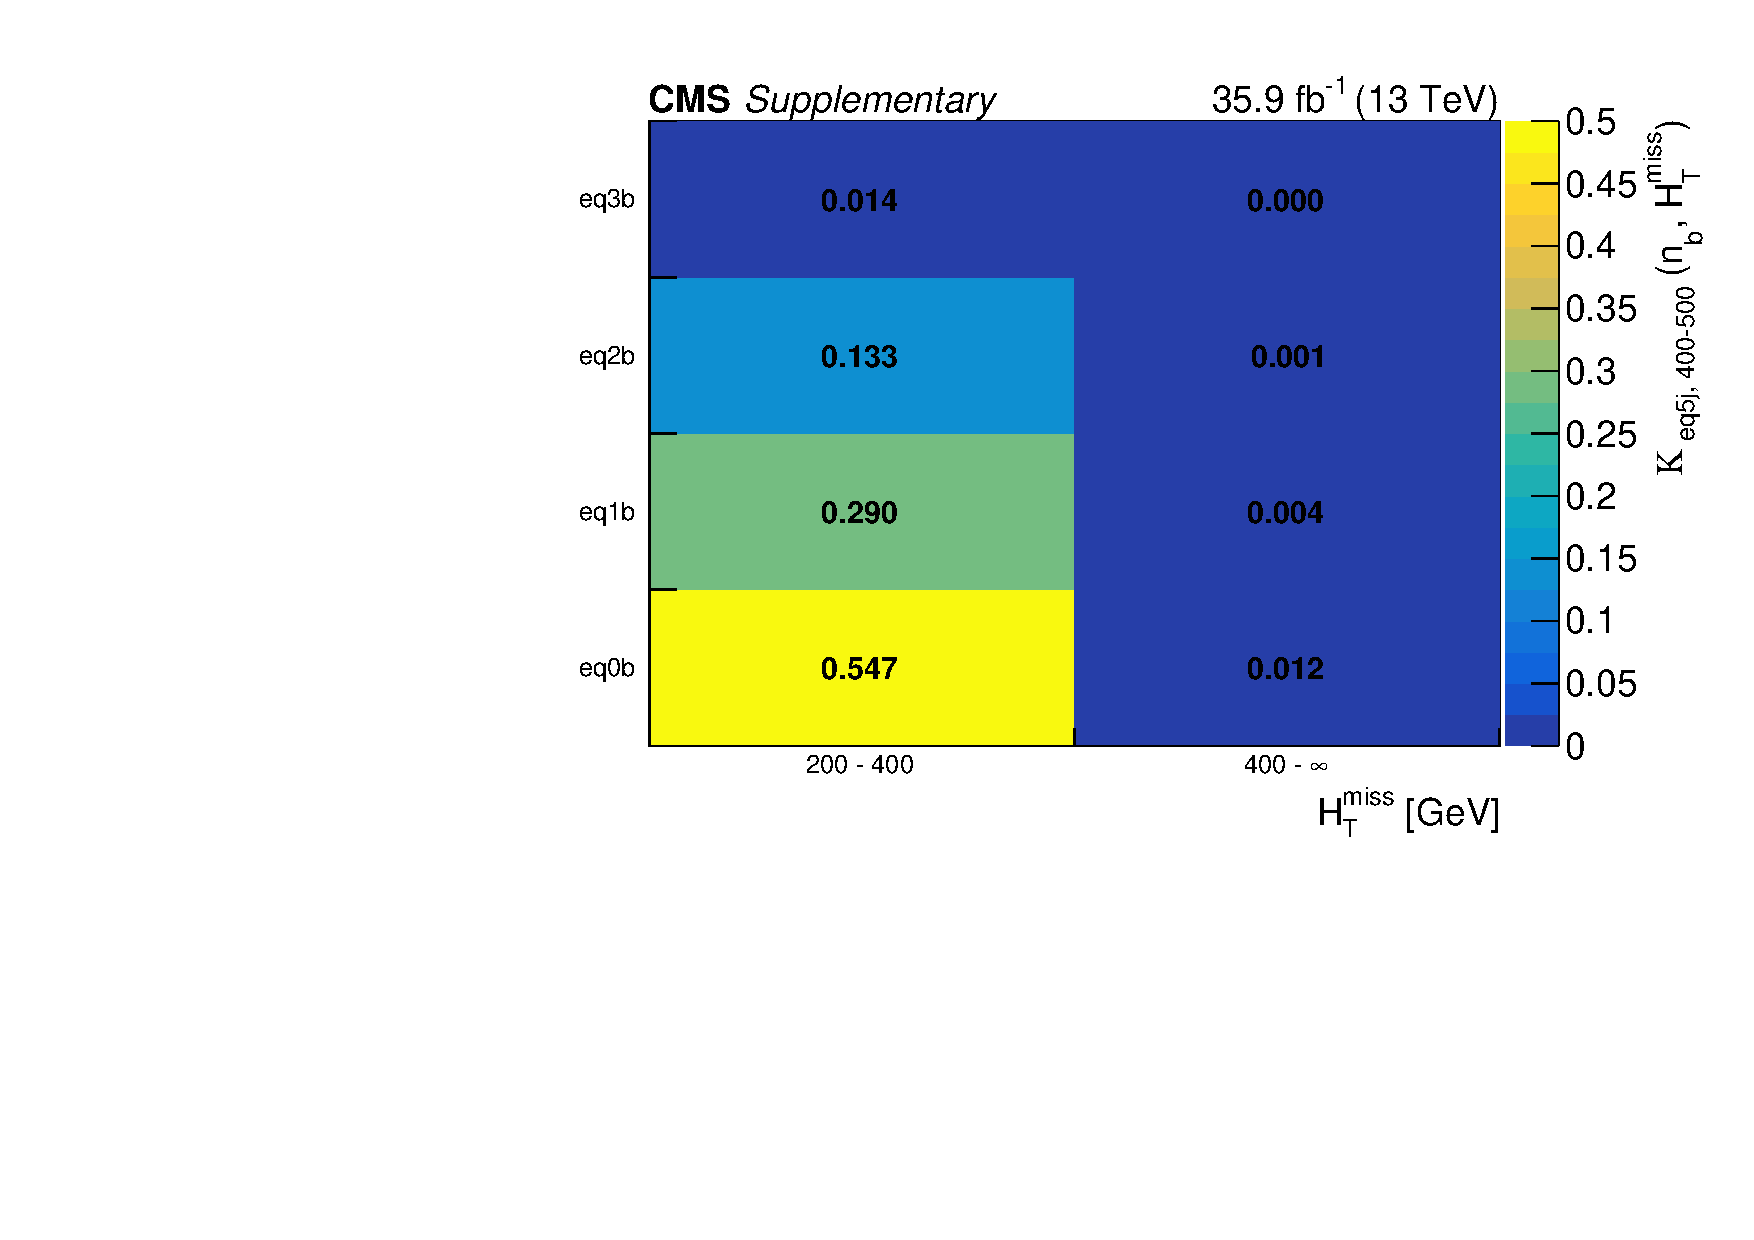
\includegraphics[width=0.3\textwidth]{figures/qcd/ewk_kappas/ewkKappa_eq5j_400-500}
    } ~~
    \subfigure[$500<\scalht<600$ \gev]{
        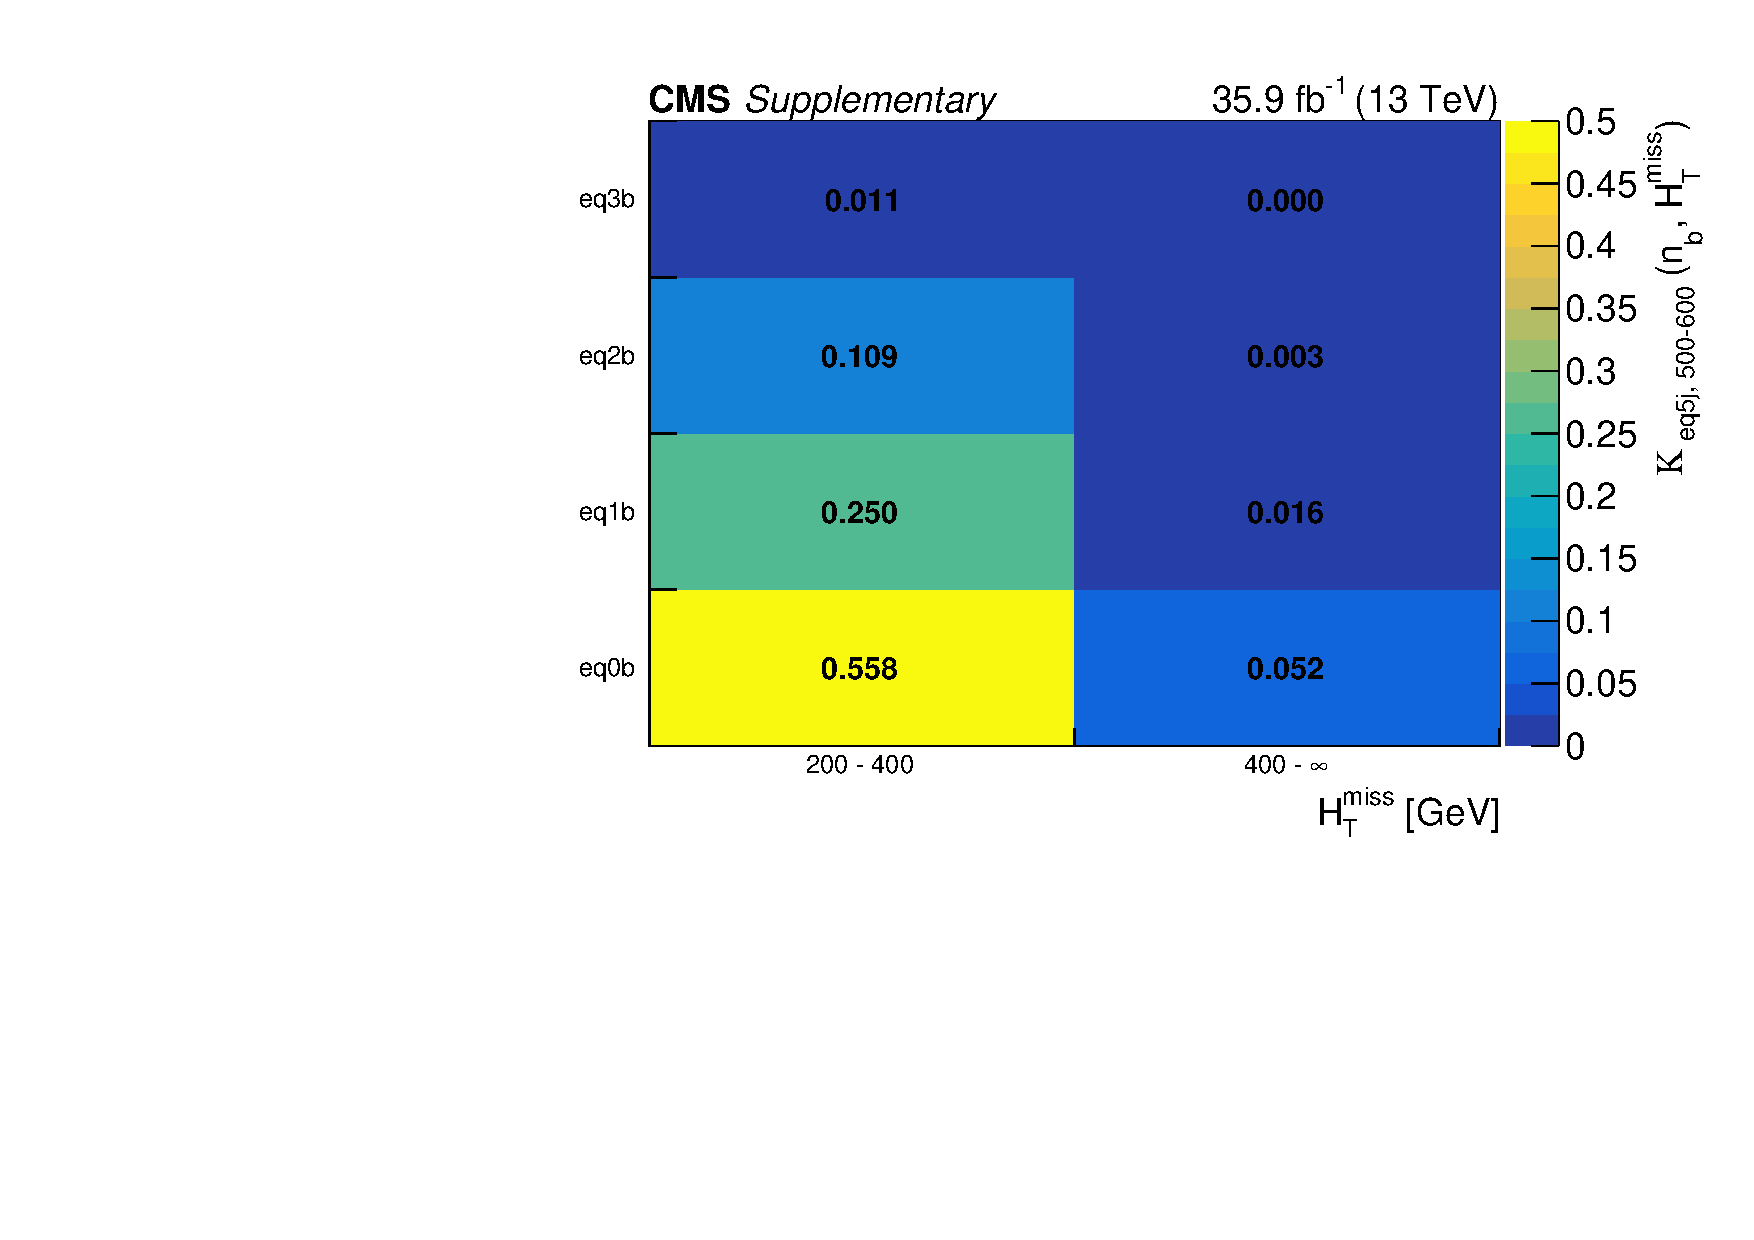
\includegraphics[width=0.3\textwidth]{figures/qcd/ewk_kappas/ewkKappa_eq5j_500-600}
    } ~~
    \subfigure[$600<\scalht<750$ \gev]{
        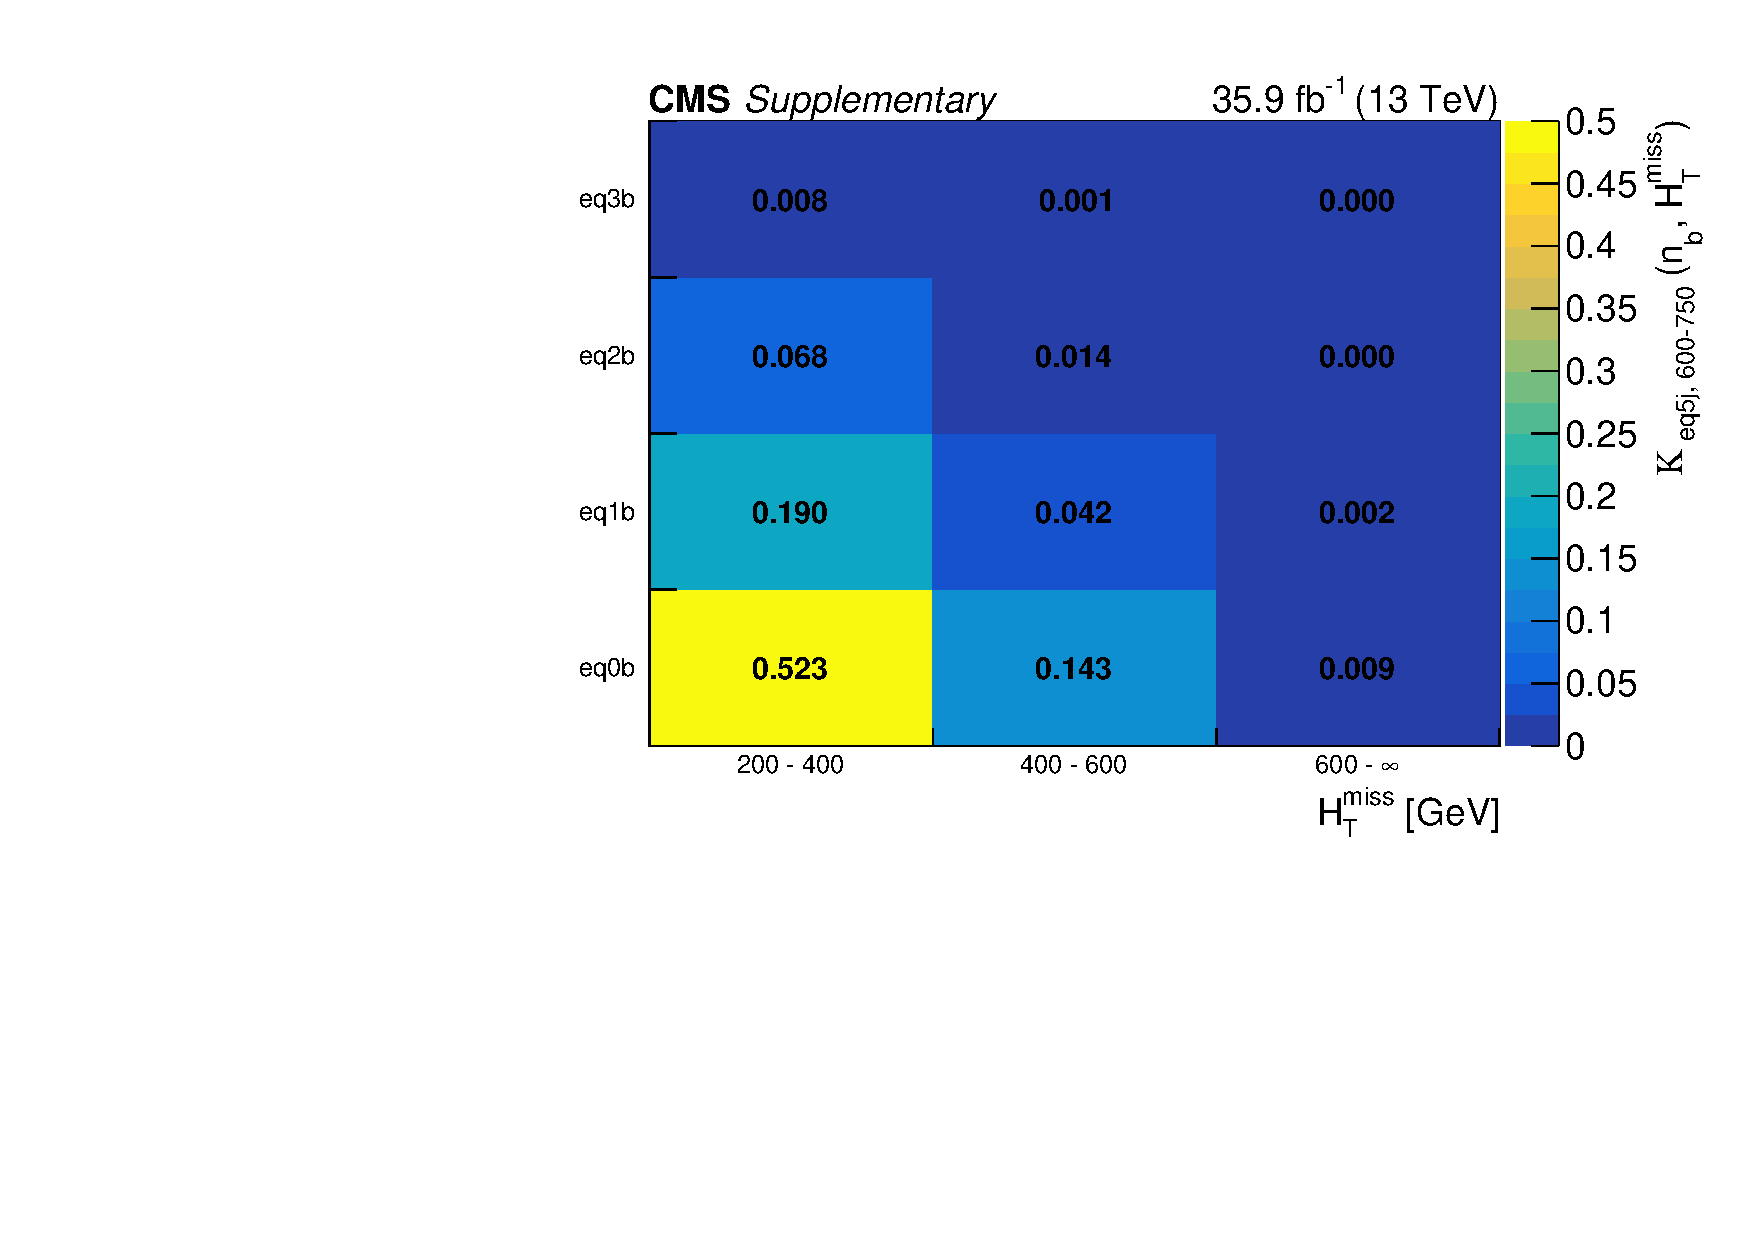
\includegraphics[width=0.3\textwidth]{figures/qcd/ewk_kappas/ewkKappa_eq5j_600-750}
    } \\
    \subfigure[$750<\scalht<900$ \gev]{
        \includegraphics[width=0.3\textwidth]{figures/qcd/ewk_kappas/ewkKappa_eq5j_750-900}
    } ~~
    \subfigure[$900<\scalht<1050$ \gev]{
        \includegraphics[width=0.3\textwidth]{figures/qcd/ewk_kappas/ewkKappa_eq5j_900-1050}
    } ~~
    \subfigure[$1050<\scalht<1200$ \gev]{
        \includegraphics[width=0.3\textwidth]{figures/qcd/ewk_kappas/ewkKappa_eq5j_1050-1200}
    } \\
    \subfigure[$400<\scalht<\infty$ \gev]{
        \includegraphics[width=0.3\textwidth]{figures/qcd/ewk_kappas/ewkKappa_eq5j_400-inf}
    } ~~
    \subfigure[$900<\scalht<\infty$ \gev]{
        \includegraphics[width=0.3\textwidth]{figures/qcd/ewk_kappas/ewkKappa_eq5j_900-inf}
    } ~~
    \subfigure[$1200<\scalht<\infty$ \gev]{
        \includegraphics[width=0.3\textwidth]{figures/qcd/ewk_kappas/ewkKappa_eq5j_1200-inf}
    } ~~
    \caption{
        Electroweak (\ttw) eq5j kappa factors used to distribute
        the QCD multijet prediction across the \nb and \mht dimensions.
    }
    \label{fig:ewk_kappas_eq5j}
\end{figure}

\begin{figure}[!h]
    \centering
    \subfigure[$400<\scalht<500$ \gev]{
        \includegraphics[width=0.3\textwidth]{figures/qcd/ewk_kappas/ewkKappa_ge6j_400-500}
    } ~~
    \subfigure[$500<\scalht<600$ \gev]{
        \includegraphics[width=0.3\textwidth]{figures/qcd/ewk_kappas/ewkKappa_ge6j_500-600}
    } ~~
    \subfigure[$600<\scalht<750$ \gev]{
        \includegraphics[width=0.3\textwidth]{figures/qcd/ewk_kappas/ewkKappa_ge6j_600-750}
    } \\
    \subfigure[$750<\scalht<900$ \gev]{
        \includegraphics[width=0.3\textwidth]{figures/qcd/ewk_kappas/ewkKappa_ge6j_750-900}
    } ~~
    \subfigure[$900<\scalht<1050$ \gev]{
        \includegraphics[width=0.3\textwidth]{figures/qcd/ewk_kappas/ewkKappa_ge6j_900-1050}
    } ~~
    \subfigure[$1050<\scalht<1200$ \gev]{
        \includegraphics[width=0.3\textwidth]{figures/qcd/ewk_kappas/ewkKappa_ge6j_1050-1200}
    } \\
    \subfigure[$400<\scalht<\infty$ \gev]{
        \includegraphics[width=0.3\textwidth]{figures/qcd/ewk_kappas/ewkKappa_ge6j_400-inf}
    } ~~
    \subfigure[$1200<\scalht<\infty$ \gev]{
        \includegraphics[width=0.3\textwidth]{figures/qcd/ewk_kappas/ewkKappa_ge6j_1200-inf}
    } ~~
    \caption{
        Electroweak (\ttw) ge6j kappa factors used to distribute
        the QCD multijet prediction across the \nb and \mht dimensions.
    }
    \label{fig:ewk_kappas_ge6j}
\end{figure}

\begin{figure}[!h]
    \centering
    \subfigure[$200<\scalht<250$ \gev]{
        \includegraphics[width=0.3\textwidth]{figures/qcd/ewk_kappas/ewkKappa_ge2a_200-250}
    } ~~
    \subfigure[$250<\scalht<300$ \gev]{
        \includegraphics[width=0.3\textwidth]{figures/qcd/ewk_kappas/ewkKappa_ge2a_250-300}
    } ~~
    \subfigure[$300<\scalht<350$ \gev]{
        \includegraphics[width=0.3\textwidth]{figures/qcd/ewk_kappas/ewkKappa_ge2a_300-350}
    } \\
    \subfigure[$350<\scalht<400$ \gev]{
        \includegraphics[width=0.3\textwidth]{figures/qcd/ewk_kappas/ewkKappa_ge2a_350-400}
    } ~~
    \subfigure[$400<\scalht<500$ \gev]{
        \includegraphics[width=0.3\textwidth]{figures/qcd/ewk_kappas/ewkKappa_ge2a_350-400}
    } ~~
    \subfigure[$500<\scalht<600$ \gev]{
        \includegraphics[width=0.3\textwidth]{figures/qcd/ewk_kappas/ewkKappa_ge2a_500-600}
    } \\
    \subfigure[$600<\scalht<750$ \gev]{
        \includegraphics[width=0.3\textwidth]{figures/qcd/ewk_kappas/ewkKappa_ge2a_600-750}
    } ~~
    \subfigure[$750<\scalht<900$ \gev]{
        \includegraphics[width=0.3\textwidth]{figures/qcd/ewk_kappas/ewkKappa_ge2a_750-900}
    } ~~
    \subfigure[$600<\scalht<\infty$ \gev]{
        \includegraphics[width=0.3\textwidth]{figures/qcd/ewk_kappas/ewkKappa_ge2a_600-inf}
    } \\
    \subfigure[$900<\scalht<\infty$ \gev]{
        \includegraphics[width=0.3\textwidth]{figures/qcd/ewk_kappas/ewkKappa_ge2a_900-inf}
    } ~~
    \caption{
        Electroweak (\ttw) ge2a kappa factors used to distribute
        the QCD multijet prediction across the \nb and \mht dimensions.
    }
    \label{fig:ewk_kappas_ge2a}
\end{figure}

\clearpage
\begin{figure}[!h]
  \centering
  \subfigure[Data counts.]{
    \includegraphics[width=0.5\textwidth]{figures/qcd/sb_mhtmet/obsYields_QcdSb}
  }
  \subfigure[Post-fit EWK background estimates.]{
    \includegraphics[width=0.5\textwidth]{figures/qcd/sb_mhtmet/postFitEwkYields_QcdSb}
  } \\
  \subfigure[Post-fit QCD background estimates.]{
    \includegraphics[width=0.5\textwidth]{figures/qcd/sb_mhtmet/postFitQcdYields_QcdSb}
  }
  \subfigure[Post-fit ML values of $\mu_{\textrm{QCD}}$.]{
    \includegraphics[width=0.5\textwidth]{figures/qcd/sb_mhtmet/rateParsQcd_QcdSb}
  } \\
  \caption{Summary of the fit result in sideband \textbf{B} ($1.25 <
    \mhtmet < 3.0$) per (\njet, \scalht) bin: (a) observed data
    counts, post-fit estimates of the contributions from the (b) EWK
    and (c) QCD processes, and (d) post-fit maximum likelihood values
    of the free parameters $\mu_{\textrm{QCD}}$.}
  \label{fig:mhtmet_sideband}
\end{figure}

\clearpage
\begin{figure}[!h]
  \centering
  \subfigure[Data counts.]{
    \includegraphics[width=0.5\textwidth]{figures/qcd/sb_bdphi/obsYields_QcdSb}
  }
  \subfigure[Post-fit EWK background estimates.]{
    \includegraphics[width=0.5\textwidth]{figures/qcd/sb_bdphi/postFitEwkYields_QcdSb}
  } \\
  \subfigure[Post-fit QCD background estimates.]{
    \includegraphics[width=0.5\textwidth]{figures/qcd/sb_bdphi/postFitQcdYields_QcdSb}
  }
  \subfigure[Post-fit ML values of $\mu_{\textrm{QCD}}$.]{
    \includegraphics[width=0.5\textwidth]{figures/qcd/sb_bdphi/rateParsQcd_QcdSb}
  } \\
  \caption{Summary of the fit result in sideband \textbf{C} ($0.2 <
    \bdphi < 0.5$) per (\njet, \scalht) bin: (a) observed data counts,
    post-fit estimates of the contributions from the (b) EWK and (c)
    QCD processes, and (d) post-fit maximum likelihood values of the
    free parameters $\mu_{\textrm{QCD}}$.}
  \label{fig:bdphi_sideband}
\end{figure}

\clearpage
\begin{figure}[!h]
  \centering
  \subfigure[Data counts.]{
    \includegraphics[width=0.5\textwidth]{figures/qcd/sb_double/obsYields_QcdSb}
  }
  \subfigure[Post-fit EWK background estimates.]{
    \includegraphics[width=0.5\textwidth]{figures/qcd/sb_double/postFitEwkYields_QcdSb}
  } \\
  \subfigure[Post-fit QCD background estimates.]{
    \includegraphics[width=0.5\textwidth]{figures/qcd/sb_double/postFitQcdYields_QcdSb}
  }
  \subfigure[Post-fit ML values of $\mu_{\textrm{QCD}}$.]{
    \includegraphics[width=0.5\textwidth]{figures/qcd/sb_double/rateParsQcd_QcdSb}
  } \\
  \caption{Summary of the fit result in the ``double'' sideband
    \textbf{A} per (\njet, \scalht) bin: (a) observed data counts,
    post-fit estimates of the contributions from the (b) EWK and (c)
    QCD processes, and (d) post-fit maximum likelihood values of the
    free parameters $\mu_{\textrm{QCD}}$.}
  \label{fig:double_sideband}
\end{figure}

\clearpage
\begin{figure}[!h]
  \centering
%  \subfigure[Pass/fail ratios \rmhtmet.]{
%    \includegraphics[width=0.5\textwidth]{figures/qcd/sb_mhtmet/signalQcdDivSbQcd_MC}
%  }
  \subfigure[QCD background estimates.]{
    \includegraphics[width=0.6\textwidth]{figures/qcd/pred/meanPredQcdYields}
  } \\
  \subfigure[EWK background estimates.]{
    \includegraphics[width=0.6\textwidth]{figures/qcd/pred/meanPredEwkYields}
  } \\
  \subfigure[Ratios of QCD and EWK background estimates.]{
    \includegraphics[width=0.6\textwidth]{figures/qcd/pred/meanPredQcdDivEwk}
  }
  \caption{The (a) weighted expected QCD background per (\njet,
    \scalht) bin, (b) the expected EWK background per bin in the
    signal region, and (c) the ratio of the QCD and EWK background
    expectations per bin. }
  \label{fig:qcd_estimate}
\end{figure}

\clearpage
\begin{figure}[!h]
  \centering
  \subfigure[$\mu_{\textrm{QCD}}$(\mhtmet) relative to $\mu_{\textrm{QCD}}$(``double'').]{
    \includegraphics[width=0.8\textwidth]{figures/qcd/val_njet_ht/rateParRatioMhtMetDivDouble1d}
  } \\
  \subfigure[$\mu_{\textrm{QCD}}$(\bdphi) relative to $\mu_{\textrm{QCD}}$(``double'').]{
    \includegraphics[width=0.8\textwidth]{figures/qcd/val_njet_ht/rateParRatioBDPhiDivDoubleSb1d}
  }
  \caption{The (fractional) level of agreement between the ML values
    for $\mu_{\textrm{QCD}}$ determined from (a) the \mhtmet and (b)
    the \bdphi sideband regions relative to those obtained from the
    ``double'' sideband region.  }
  \label{fig:qcdVal}
\end{figure}

\clearpage
\begin{figure}[!h]
  \centering
  \subfigure[Multijet and non-multijet yields per $(\njet, \nb)$.]{
    \includegraphics[width=0.5\textwidth]{figures/qcd/shapes/QcdSb/yield_njet_bjet.png}
  }
  \subfigure[Multijet and non-multijet \nb shapes per \njet bin.]{
    \includegraphics[width=0.5\textwidth]{figures/qcd/shapes/QcdSb/norm_njet_bjet.png}
  } \\
  \subfigure[Ratio of multijet to non-multijet \nb shapes.]{
    \includegraphics[width=0.5\textwidth]{figures/qcd/shapes/QcdSb/ratio_njet_bjet.png}
  }
  \caption{Sideband \textbf{B} multijet and non-multijet distributions
    categorised in $(\njet, \nb)$ bins, corrected by rate parameters
    from the fit in the QCD sidebands. The (a) rate parameter corrected yields,
    (b) \nb shapes per \njet (i.e. each \njet bin is normalised to unity) and
    (c) the ratio of multijet to non-multijet of \nb shapes are shown.}
  \label{fig:qcd_nb_shapes_mhtmetsb}
\end{figure}

\begin{figure}[!h]
  \centering
  \subfigure[Multijet and non-multijet yields per $(\scalht, \HTmiss)$.]{
    \includegraphics[width=0.5\textwidth]{figures/qcd/shapes/QcdSb/yield_ht_mht.png}
  }
  \subfigure[Multijet and non-multijet \HTmiss shapes per \scalht bin.]{
    \includegraphics[width=0.5\textwidth]{figures/qcd/shapes/QcdSb/norm_ht_mht.png}
  } \\
  \subfigure[Ratio of multijet to non-multijet \HTmiss shapes.]{
    \includegraphics[width=0.5\textwidth]{figures/qcd/shapes/QcdSb/ratio_ht_mht.png}
  }
  \caption{Sideband \textbf{B} multijet and non-multijet distributions
    categorised in $(\scalht, \HTmiss)$ bins, corrected by rate parameters
    from the fit in the QCD sidebands. The rate parameter corrected yields
    are shown in (a), \HTmiss shapes per \scalht (i.e. each \scalht bin is normalised
    to unity) are shown in (b) and the ratio of multijet to non-multijet of
    \HTmiss shapes are shown in (c). The \scalht and \HTmiss values on the
    abscissa represents the lower bin boundary. The next bin gives the upper
    bin boundary (if the upper edge is bounded). The multijet component in
    sideband \textbf{B} resides in low \HTmiss bins.}
  \label{fig:qcd_mht_shapes_mhtmetsb}
\end{figure}

\clearpage
\begin{figure}[!h]
  \centering
  \subfigure[Multijet and non-multijet yields per $(\njet, \nb)$.]{
    \includegraphics[width=0.5\textwidth]{figures/qcd/shapes/BDPhiSb/yield_njet_bjet.png}
  }
  \subfigure[Multijet and non-multijet \nb shapes per \njet bin.]{
    \includegraphics[width=0.5\textwidth]{figures/qcd/shapes/BDPhiSb/norm_njet_bjet.png}
  } \\
  \subfigure[Ratio of multijet to non-multijet \nb shapes.]{
    \includegraphics[width=0.5\textwidth]{figures/qcd/shapes/BDPhiSb/ratio_njet_bjet.png}
  }
  \caption{Sideband \textbf{C} multijet and non-multijet distributions
    categorised in $(\njet, \nb)$ bins, corrected by rate parameters
    from the fit in the QCD sidebands. The rate parameter corrected yields
    are shown in (a), \nb shapes per \njet (i.e. each \njet bin is normalised
    to unity) are shown in (b) and the ratio of multijet to non-multijet of
    \nb shapes are shown in (c).}
  \label{fig:qcd_nb_shapes_bdphisb}
\end{figure}

\begin{figure}[!h]
  \centering
  \subfigure[Multijet and non-multijet yields per $(\scalht, \HTmiss)$.]{
    \includegraphics[width=0.5\textwidth]{figures/qcd/shapes/BDPhiSb/yield_ht_mht.png}
  }
  \subfigure[Multijet and non-multijet \HTmiss shapes per \scalht bin.]{
    \includegraphics[width=0.5\textwidth]{figures/qcd/shapes/BDPhiSb/norm_ht_mht.png}
  } \\
  \subfigure[Ratio of multijet to non-multijet \HTmiss shapes.]{
    \includegraphics[width=0.5\textwidth]{figures/qcd/shapes/BDPhiSb/ratio_ht_mht.png}
  }
  \caption{Sideband \textbf{C} multijet and non-multijet distributions
    categorised in $(\scalht, \HTmiss)$ bins, corrected by rate parameters
    from the fit in the QCD sidebands. The rate parameter corrected yields
    are shown in (a), \HTmiss shapes per \scalht (i.e. each \scalht bin is normalised
    to unity) are shown in (b) and the ratio of multijet to non-multijet of
    \HTmiss shapes are shown in (c). The \scalht and \HTmiss values on the
    abscissa represents the lower bin boundary. The next bin gives the upper
    bin boundary (if the upper edge is bounded). Similarly to
    sideband \textbf{B}, the multijet component in sideband \textbf{C}
    resides in low \HTmiss bins.}
  \label{fig:qcd_mht_shapes_bdphisb}
\end{figure}

\clearpage
\begin{figure}[!h]
  \centering
  \subfigure[Multijet and non-multijet yields per $(\njet, \nb)$.]{
    \includegraphics[width=0.5\textwidth]{figures/qcd/shapes/DoubleSb/yield_njet_bjet.png}
  }
  \subfigure[Multijet and non-multijet \nb shapes per \njet bin.]{
    \includegraphics[width=0.5\textwidth]{figures/qcd/shapes/DoubleSb/norm_njet_bjet.png}
  } \\
  \subfigure[Ratio of multijet to non-multijet \nb shapes.]{
    \includegraphics[width=0.5\textwidth]{figures/qcd/shapes/DoubleSb/ratio_njet_bjet.png}
  }
  \caption{Sideband \textbf{A} multijet and non-multijet distributions
    categorised in $(\njet, \nb)$ bins, corrected by rate parameters
    from the fit in the QCD sidebands. The rate parameter corrected yields
    are shown in (a), \nb shapes per \njet (i.e. each \njet bin is normalised
    to unity) are shown in (b) and the ratio of multijet to non-multijet of
    \nb shapes are shown in (c).}
  \label{fig:qcd_nb_shapes_doublesb}
\end{figure}

\begin{figure}[!h]
  \centering
  \subfigure[Multijet and non-multijet yields per $(\scalht, \HTmiss)$.]{
    \includegraphics[width=0.5\textwidth]{figures/qcd/shapes/DoubleSb/yield_ht_mht.png}
  }
  \subfigure[Multijet and non-multijet \HTmiss shapes per \scalht bin.]{
    \includegraphics[width=0.5\textwidth]{figures/qcd/shapes/DoubleSb/norm_ht_mht.png}
  } \\
  \subfigure[Ratio of multijet to non-multijet \HTmiss shapes.]{
    \includegraphics[width=0.5\textwidth]{figures/qcd/shapes/DoubleSb/ratio_ht_mht.png}
  }
  \caption{Sideband \textbf{A} multijet and non-multijet distributions
    categorised in $(\scalht, \HTmiss)$ bins, corrected by rate parameters
    from the fit in the QCD sidebands. The rate parameter corrected yields
    are shown in (a), \HTmiss shapes per \scalht (i.e. each \scalht bin is normalised
    to unity) are shown in (b) and the ratio of multijet to non-multijet of
    \HTmiss shapes are shown in (c). The \scalht and \HTmiss values on the
    abscissa represents the lower bin boundary. The next bin gives the upper
    bin boundary (if the upper edge is bounded). As with the other sidebands,
    the multijet component in sideband \textbf{A} resides in low \HTmiss
    bins, apart from high \scalht where some events extend to high \HTmiss.}
  \label{fig:qcd_mht_shapes_doublesb}
\end{figure}
